%  University of Houston PhD proposal and dissertation
%
% on  PC
%\documentclass[12pt]{report}
% \usepackage{uhthesis}
% \usepackage[pctex32]{graphics}
% \usepackage[pctex32]{color}
%\usepackage{psfig}
\documentclass[12pt]{report}
\usepackage{uhthesis3}
\usepackage{epsfig}
\usepackage{epsf}
\usepackage[hidelinks]{hyperref}
\usepackage{subfigure}

\usepackage{amsmath}
\usepackage{algorithm}
\usepackage[noend]{algpseudocode}
\usepackage{listings}


% LAD definitions
\def\vx{{\vec x}}
\def\vxdot{{\dot\vx}} \def\vxddot{{\ddot\vx}}
\def\tpose{^\top}
\def\ru{{\rm u}}
\def\vc{{\vec c}}
\def\vrho{{{\bf p}}}
\def\mat#1{{\bf#1}}
\def\vec#1{{\bf#1}}
\def\bold#1{\setbox0=\hbox{#1}
 \kern-.025em\copy0\kern-\wd0
 \kern.05em\copy0\kern-\wd0
 \kern-.025em\raise.0433em\box0}
\def\vsigma{{\bf \sigma}}
\def\vepsilon{{\bf \epsilon}}
\def\ssqueeze{\vspace{-0.5cm}}

\def\bsqueeze{\vspace*{-0.8cm}}
\def\bpsqueeze{\vspace*{-0.6cm}}
\def\asqueeze{\vspace{-0.5cm}}


\def\inv{^{-1}}
\def\vuhat{{\hat \vec u}}
\def\avtk{{t_{k}}}
\def\bvtk{{t_{k+1}}}
\def\vu{{\vec u}}
\def\vuhat{{\hat \vec u}}
\def\vq{{\vec q}}
\def\vqdot{{\dot\vq}}
\def\tpose{^\top}
\def\mat#1{{\bf#1}}
\def\extvec#1#2#3{{~^{#1}{\bf#2}_{#3}}}
\def\extvecrm#1#2#3{{~^{{\rm #1}}{\bf#2}_{#3}}}

\def\cavindex{{\cal V\cal I}}
\def\caawpoint{{\extvec{\Phi}{x}{j}}}
\def\caaipointrm{{\extvecrm{I}{x}{j}}}
\def\caaipoint{{\extvec{I}{x}{j}}}

\newcounter{lfigcounter}
\newenvironment{IonTab}{\begin{table}[htb]}{\end{table}}
\newenvironment{IonFig}{\setcounter{lfigcounter}{1}\begin{figure}}{\end{figure}}
\newenvironment{IonFigH}{\setcounter{lfigcounter}{1}\begin{figure}[h]}{\end{figure}}
\newenvironment{IonFigT}{\setcounter{lfigcounter}{1}\begin{figure}[t]}{\end{figure}}
\def\ionbox#1{\makebox[#1]{(\alph{lfigcounter})}\stepcounter{lfigcounter}}

%%%%%%%%%%%%%%%%%%%%%%%%%%%%%%%%%%%%%%%%%%%%%%%%%%%%%%%%%%%%%%5

%\input{algorithms}
%
%
%
% on UNIX LATEX and Windows PCTEX32
%\documentstyle[12pt,uhthesis1,psfig]{report}
%\usepackage{epsfig}
%\input{algorithms}
%\input{psfig}
%\input{dnmmath}
%\input{ion-math}

\setcounter{secnumdepth}{4}
\begin{document}

\title{\bf \large Scalable Data Visualization Methods\\ for Academic Careers }
\author{Kyeongan Kwon}
\submitdate{August 2016} \degree{Doctor of Philosophy}{Dissertation}
\adviser{Dr. Ioannis Pavlidis, Chairman\\
Department of Computer Science\\
University of Houston }

\firstreader{Dr. Zhigang Deng\\
Department of Computer Science\\
University of Houston}

\secondreader{Dr. Guoning Chen\\
Department of Computer Science\\
University of Houston }

\thirdreader{Dr. Brian Uzzi\\
Kellogg School of Management \\
Northwestern University }

%\fourthreader{}


\copyrightfalse \makecoverpages
\begin{acknowledgements}
\begin{center}
   {\bf ACKNOWLEDGEMENTS}\\
\end{center}


I would like to give my deepest gratitude towards Dr. Ioannis Pavlidis, who has been guiding me through my research. He has given me numerous opportunities throughout my PhD years, and always shared his views and experience in several of the projects that I worked upon. The amount of knowledge and experience I have gained from him is priceless.\\

\noindent
I want to thank all my committee members, Dr. Zhigang Deng, Dr. Guoning Chen, and Dr. Brian Uzzi for their advice and feedback making this research possible. Also, I thank all lab members for being my colleagues and friends; especially, Dinesh Majeti, whom I have been working closely with.\\

\noindent
Last but not least, my family is the backbone of my success. Being able to continue my education in America was only a dream. And to this very day, I cannot believe I was able to fulfill my dream. It is all thanks to my family. Although we are miles away and seas apart, my family made me feel as if I were home. I cannot be more thankful for their unconditional love, encouragement, motivation, and support.

\end{acknowledgements}

\begin{abstract}
Evaluation of scholarly achievements in academia is largely based on the researcher's publication record. This record is communicated in exhaustive detail in the researcher's curriculum vitae (CV) or in summary via her/his {\it h}-index. The {\it h}-index, although a convenient abstraction, considers neither the time of the publication nor the impact factor ($IF$) of the journal where it appeared. In this article we present a novel method that visually complements the {\it h}-index, revealing at a glance the nature of a researcher's scholastic record. This method (aka Scholar Plot) is particularly appropriate for web interfaces, as it produces information that is compact and simple, yet highly illuminating. The method uses Google Scholar, Impact Factor and NSF/NIH Funding data to create a temporal representation of a researcher's publication/funding record that blends publication prestige with paper popularity and funding information. Scholar Plot aids to obtain an insightful appraisal of academics at one's fingertips.

%User studies have been growing larger in terms of size and duration. This is an exciting development because user studies are realistically performed beyond the lab environments. Yet, these studies are challenging because researchers have to organize and analyze large amounts of data. Proper statistical analysis is critical and has received a lot of attention. One aspect that has been neglected is a visual interface to the study's results. Such an interface can support qualitative understanding, conveying at a glance studies of sympathetic responses. A case in point is the student exam study that we discuss in this research. One challenge that such a research faces is effective visualization of the study data (e.g., physiological data) that otherwise requires technical expertise to comprehend. Another challenge is the multidimensionality of the study data. Static snapshots (e.g., performance data) and dynamic evolution (e.g., physiological data) have to be visualized at a glance. Moreover, the visualization scheme should take into account spatiotemporal aspect of the examination by presenting study results from multiple subjects over a period. In this research we propose a set of designing principles for effective visualization of the study results. The designing principles are evaluated on the student exam study which aims is to understand students' stress patterns while taking course exams. In particular, a visualization interface is developed as per the designing principles to comprehend the exam study results at a glance. The interface represents voluminous data in a way that the users with little domain specific knowledge can be able to derive meaningful conclusions. It effectively displays the students' course performance data and their stress profile in one glance. The interface also allows inter-subject and intra-subject comparisons in a few mouse clicks or finger taps.


%There has been proliferation of mixed methods in user studies. At the same time, user studies have been growing larger in terms of size and duration. This is enthusiasm in such that experimental designs are realistic but also challenging. Researchers have to organize and analyze large amounts of data. Proper statistical analysis is critical and has received a lot of attention. One aspect that has been neglected is a visual interface to the study's results. Such an interface can support qualitative understanding, conveying at a glance the studies of sympathetic responses in students taking exams either on paper vs. tablets.
%
%\bigskip
%\noindent
%Additionally, data from a specialized domain (e.g. physiology data) may not be intuitive to users who have no prior experience with such domain. Therefore there needs to be a way to represent voluminous data in a way that the average users can comprehend and be able to derive meaningful conclusions.
%
%\bigskip
%\noindent
%We introduce an effective visualization methods to conduct large scale physiology data at a glance. This universial design scheme will be expanded upon various types of experiments. Spacial-temporal approaches for comparisons between two observations will be proved and it is exceptionally useful. Furthermore, instinctive visualization may be used for users from neophytes to experts.





\end{abstract}
\setlength{\parskip}{.1 in}

\makecontentspages

%uncomment the following for single space drafts
%\singlespace

% \pagenumbering{romans}{1}
% \beforepreface

%\pagestyle(empty}


%%%%%%%%%%%%%%%%%%%%%%%%%%%%%%%%%%%%%%%%%%%%%%%%%%%%%%%%%%%%%%%%%%%%


% \input{chapter0Nomenclature.tex}
% \setcounter{page}{0}

\chapterpages

%turn figures on and off
\newif \ifFIGS

%\FIGStrue

\FIGSfalse


% to fix the page number
%\input{Sample_chapter.tex}
%\input{table.tex}
\chapter{Introduction}\label{chap:Intro}

In the world of Internet and apps there is a tendency to measure nearly everything, displaying publicly visual impressions of these measurements. Familiar symbols include star ratings of movies and restaurants, thumps up/down ratings of opinion articles, and counting distributions of site visits. Visualization of professional records is increasingly part of the fray - see for example, fancy letter ratings for service providers in Angie's List\textsuperscript{TM}. 

A lot of these measures are based on crowdsourcing or on online data, which explains their phenomenal proliferation in the Internet and app space. Their succinct visualizations provide easily digestible cues, conditioning users' attitudes towards specific shows or services. One could argue that such summary visualizations may be an oversimplification. This is probably true and something that can be  fixed with more research on multi-faceted measures and their display. At the same time, even simple data visualizations provide valuable information to the user, who could not even imagine it in the Yellow Pages era, just a few years ago. 

Professional records of distinct interest for measurement and display are the academic records. First, they differ from other records because they can be objectively quantified to a large degree. Second, they are multi-faceted and often prolific, presenting a challenge to succinct visualization. Third, they are of great social value, as academic research and education are valuable resources, about which the users (students, faculty, and funding agencies) can never have enough information.

It is relatively difficult and time consuming to thoroughly analyze academic CVs. Hence, graduate students in search of a Ph.D. advisor, aspiring faculty in search of a fitting department, and reviewers in a funding agency assessing a proposer's record can use help through an appropriate interface. Such help has been rendered in small doses the last few years with the advent of several publicly available tools. In a practical sense, the end effect of such help, would be no different than the benefit the movie-goer and restaurant-goer have already been receiving.

To quantify academic careers, some researchers focused on a quest for a `number' that sums up an individual's scholarship. The most well-known outcome of this line of research is the {\it h}-index, proposed by Hirsch \cite{Hirsch:2005}. Despite its value, the {\it h}-index has weaknesses and when used, context should be carefully taken into account; such context includes the academic field and the academic age of the candidate \cite{Bornmann:2009}. Other efforts focused on visualizing citation patterns \cite{Chen:2001, Leydesdorff:2007} - an important measure of impact. Envision \cite{Nowell:1997} and PaperCube \cite{Bergstrom:2009} provide to users visualization tools to explore patterns in the literature. PaperLens \cite{Lee:2005} introduced a novel visualization scheme for eight years of InfoVis and 23 years of CHI conference proceedings.
A social tool named Scholarometer has been developed to facilitate citation analysis and to evaluate the impact of authors \cite{Kaur:2014}.
SciVal \cite{Vardell:2011} summarizes researchers' profiles using Scopus, clustering them under departmental links.  It offers search capabilities that aim to facilitate the formation of collaborative teams by rendering matches between experts easier.

In this article, I introduce \href{http://scholarplot.com}{Scholar Plot (SP)}, a comprehensive yet compact visual interface for academic scholarship. SP scales up across the academic space, covering not only academics, but also the departments and colleges they belong to. Importantly, SP features multi-faceted information, bringing to the fore different strengths and weaknesses of individual and group records. This information includes publications, citations, impact factors, and funding. Last but not least, SP is freely available and is based on public  data that are as inclusive as possible. This is in contrast to  company-owned scientometrics tools with restricted access, which are based on less inclusive data sets; case in point is Elsevier's Scopus that generally does not cover the full citation space. The combination of all these characteristics makes SP a unique interface of academic merit. 


% ==================================================
\chapter{Related Work}\label{chap:Related Work}
% ==================================================

There has been work on the quantification of academic careers, focused on a quest for a `number' that sums up an academic's scholarship. The most well-known outcome of this line of research is the {\it h}-index, proposed by Hirsch \cite{Hirsch:2005}. A scholar has an index of {\it h} if s/he has published {\it h} papers each of which has been cited in other papers at least {\it h} times (Figure \ref{fig-hindex}).

\begin{figure*}
    \centering
    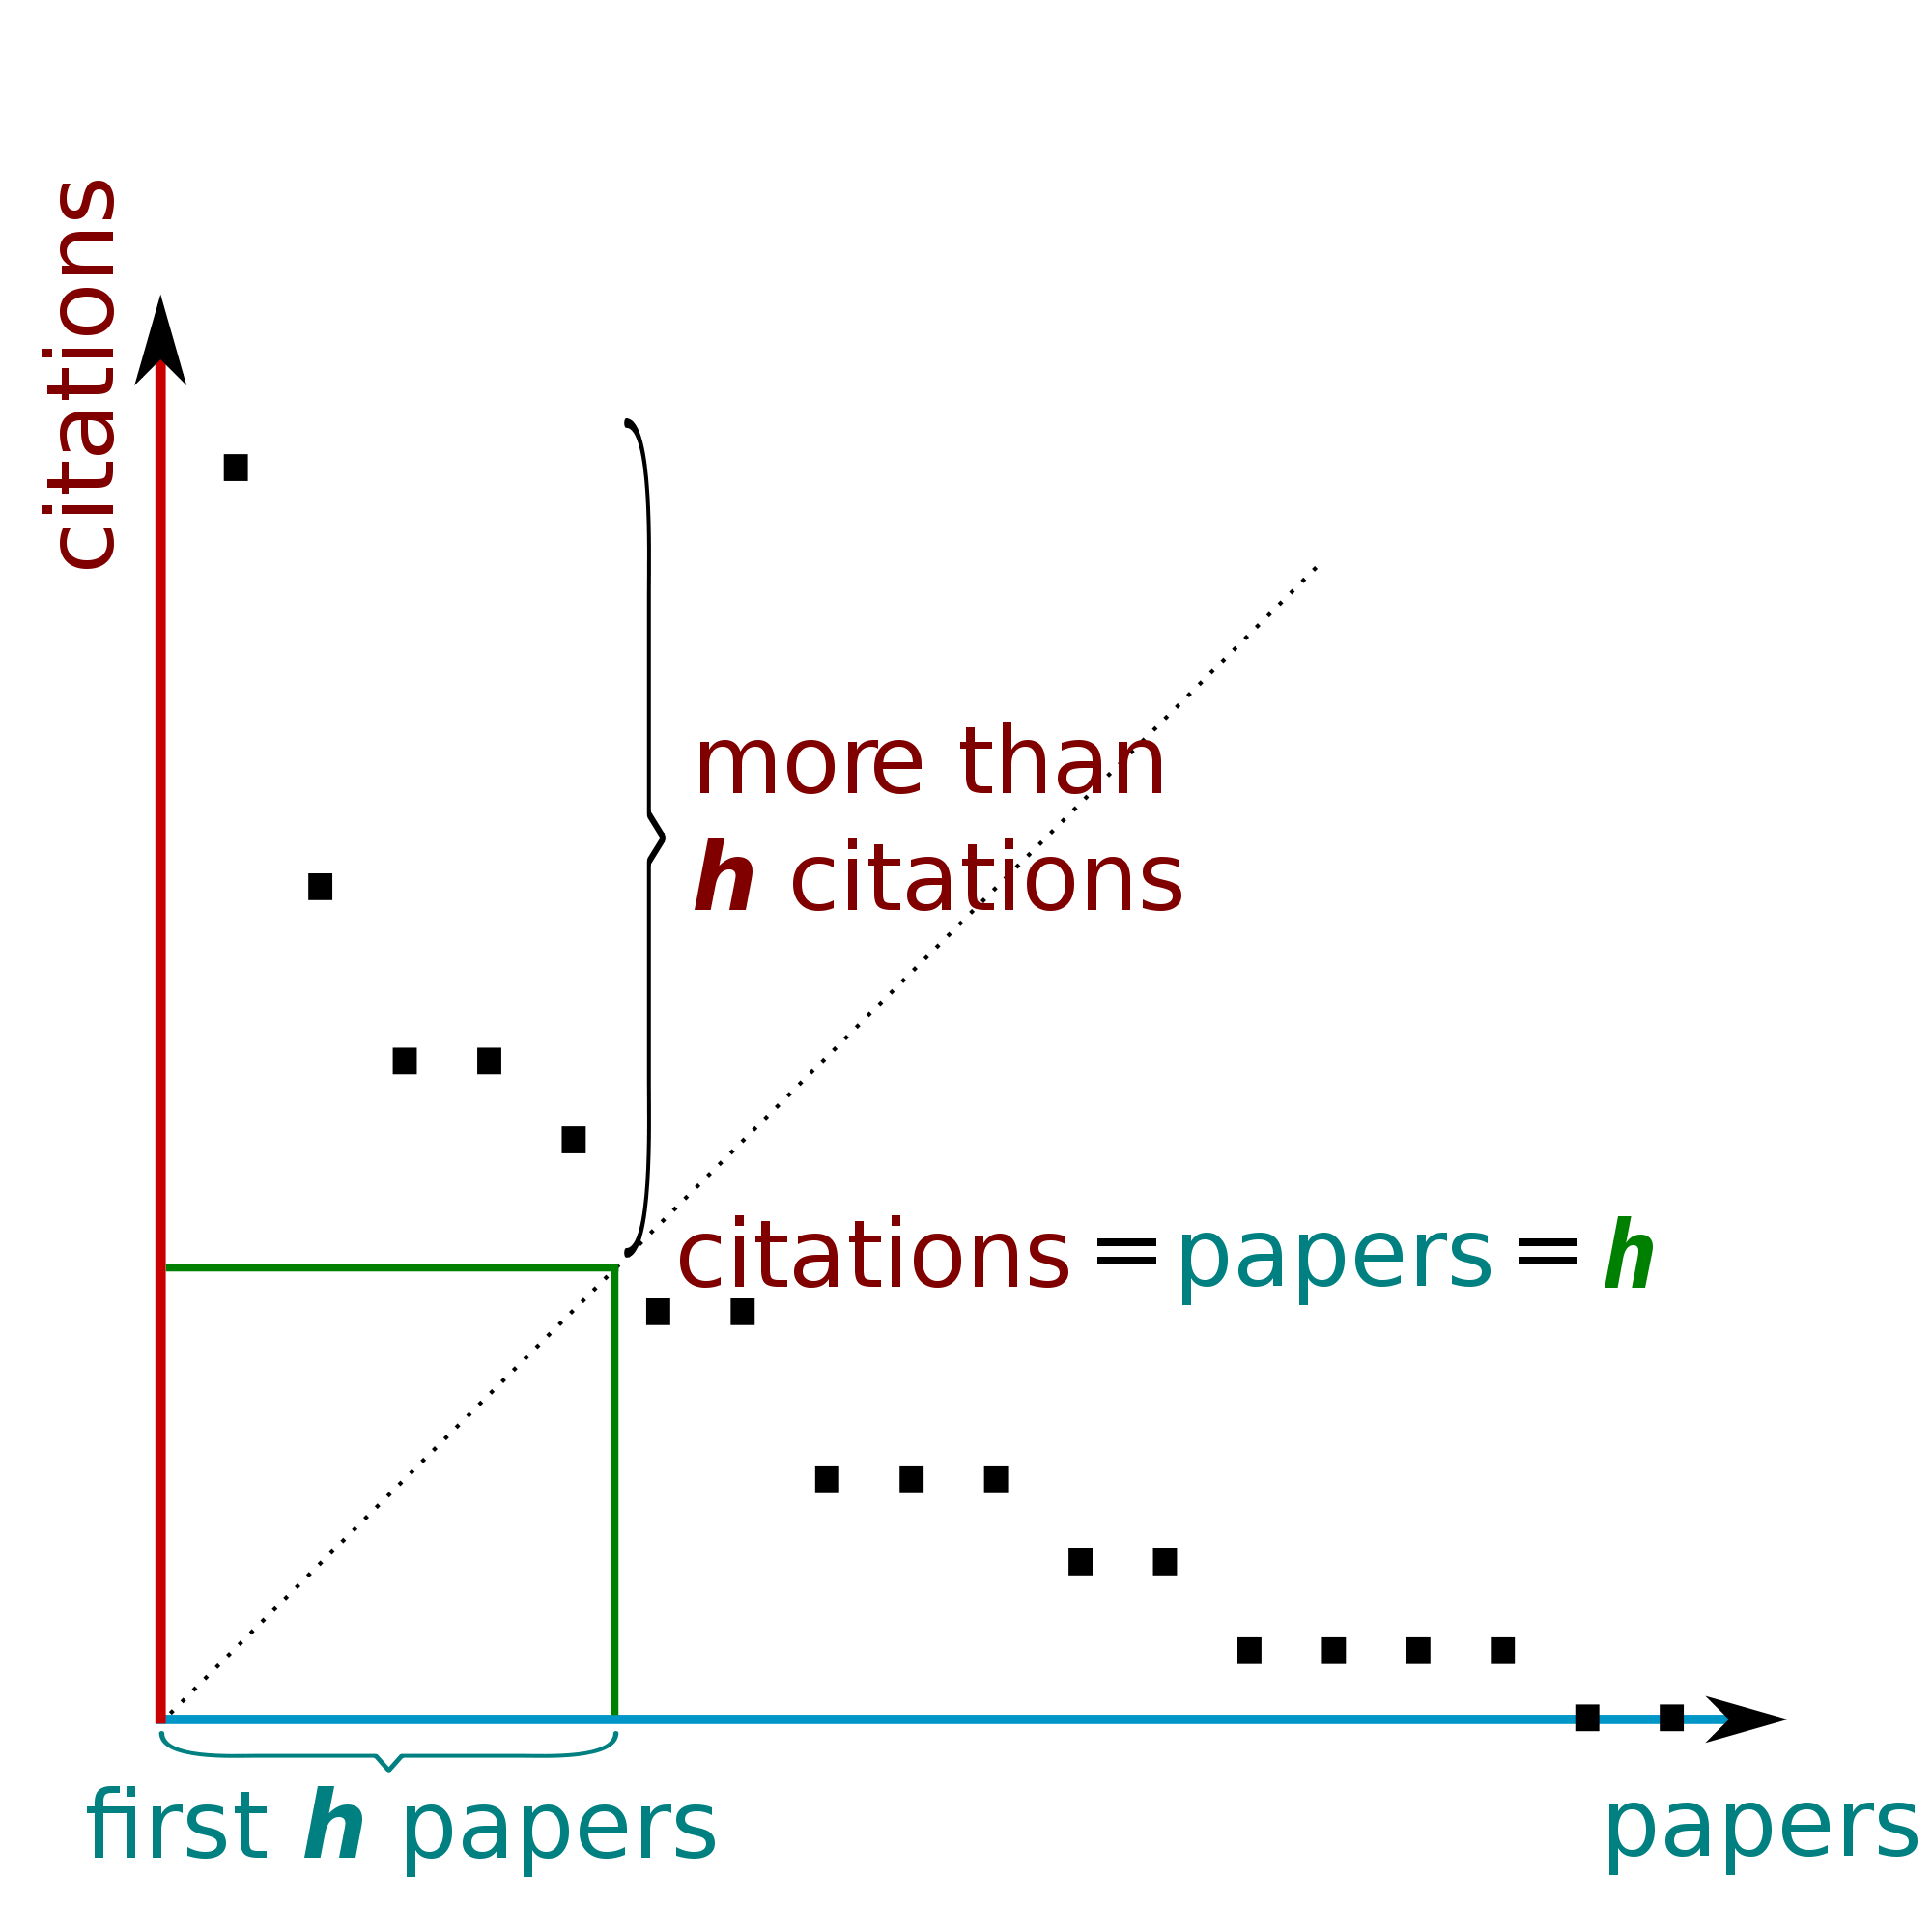
\includegraphics[width=.3\textwidth]{figures/H-index.png}
    \caption{h-index from a plot of decreasing citations for numbered papers.}~\label{fig-hindex}
\end{figure*}


The {\it h}-index depends on both the number of publications and the number of citations. Hirsch demonstrated that {\it h} can predict honors, such as the National Academy membership and the Nobel prize. He also suggested that it could predict advancement to tenure, although with some uncertainty.
Despite its value, the {\it h}-index has weaknesses and when used, context should be carefully taken into account; such context includes the academic field and the academic age of the candidate \cite{Bornmann2}.

With the advent of Google Scholar \cite{Googl82:online}, information about a researcher's publication record and her/his {\it h}-index has become easily accessible. Then, with the ease of access of the internet, this information has become ubiquitous.

In this dissertation, I introduce data visualization methods that complement publication information contained in a standard CV and summarized by the {\it h}-index. The tool produces a temporal visualization that connects the {\it h}-index with the paper citations and the journal impact factors along with funding data.

There have been other efforts in visualizing patterns of scientific production and impact \cite{Katy:2010, Chen:2001, Leydesdorff:2007}. Recently, a mobile app (DBIScholar) has also appeared that interfaces information from Google Scholar \cite{sabrina741}. A social tool named Scholarometer has been developed to facilitate citation analysis and to evaluate the impact of authors \cite{Kaur:2014}. This tool helps to visualize author and discipline networks. There is another tool called SciVal Expert, which visualizes the collaboration and research output of institutions \cite{Vardell:2011}. This tool uses data from Elsevier's Scopus, the largest abstract and citation database of peer-reviewed literature \cite{Scopu91:online}. However, these tools do not provide a visual picture of a single scholar's achievements.

The method and application differ from the prior art. At a glance, Scholar Plot helps the reviewer determine where the researcher's impact (if any) arises from.% : citations in articles published in low impact journals or citations in articles published in high impact journals.

Students need more information to decide about their college. Nowadays, a university has a ranking as well as each department with each college in that university. So students need publicly accessible information which is cheap and get a summary of various measures being used to evaluate faculty. Rankings are used to make choices to avoid risks of joining lower ranking colleges \cite{mcdonough1998college}.

The goal of research is to articulate a clear, comprehensive, and measurable performance evaluation scheme for academics. This scheme should reveal causal relationships among the merit criteria. This research provides a summary interface to facilitate executive decisions. The tool produces a temporal visualization that connects the {\it h}-index with the paper citations, and the journal impact factors along with funding data. Scholar Plot helps the reviewer determine at a glance where the researcher's impact (if any) arises from.


Here, I introduce a data visualization tool that complements the US News Rankings and the publication information contained in a standard CV. Visualization facilitates access to data and supports actionable insights \cite{Yi:2008:UCI}. It also helps to bring out patterns and pattern violations in the underlying data.
%The tool produces a temporal visualization that connects the {\it h}-index with the paper citations and the impact factors along with the funding data. Our method and application differ from the prior art. Scholar Plot helps the reviewer determine at a glance from where the researcher's impact (if any) arises from. It also gives a hierarchical view of accomplishments from a single author to the department to the entire college.
\chapter{Methodology}\label{chap:Methods }


% =============================================================================
\section{Visualization and User Interface}
% =============================================================================
Scholar Plot obtains the Impact Factor ($IF$) for a particular journal from our database. The data of Impact Factor is acquired from The Thomson Reuters Impact Factor - Web of Science. Based on all this information it constructs the plots as per the design outlined in the Visualization and User Interface section, using nvd3 library \cite{nvd3org}.


The NSF/NIH/NASA funding datasets are available at the respective US government websites in various file formats such as XML, CSV and so on \cite{nsf, nih}. We implemented a script to parse this massive XML dataset into our data structure that consists of AwardID, AwardAmount, First name, Last name, Investigator by RoleCode (Principal Investigator, Co-Principal Investigator and Former Principal Investigator), using XMLStarlet \cite{XMLStarlet}. We imported this data to our database using Toad DBMS tool. %We designed our relational database schema in MySQL.

\begin{figure}%[!htb]
\centering
  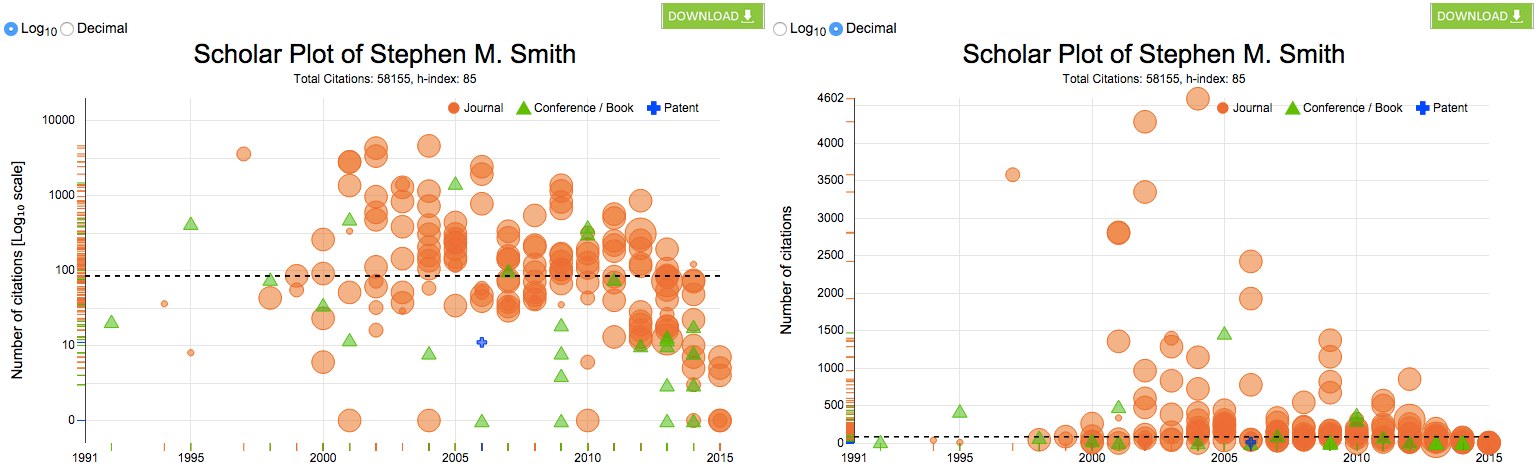
\includegraphics[width=1\columnwidth]{figures/fig_scaleView}
  \caption{The $log_{10}$ view and $decimal$ view: The radio button allows to switch between different scale views without reloading the entire page.}~\label{fig:fig-scale}
\end{figure}

\begin{figure*}
  \centering
  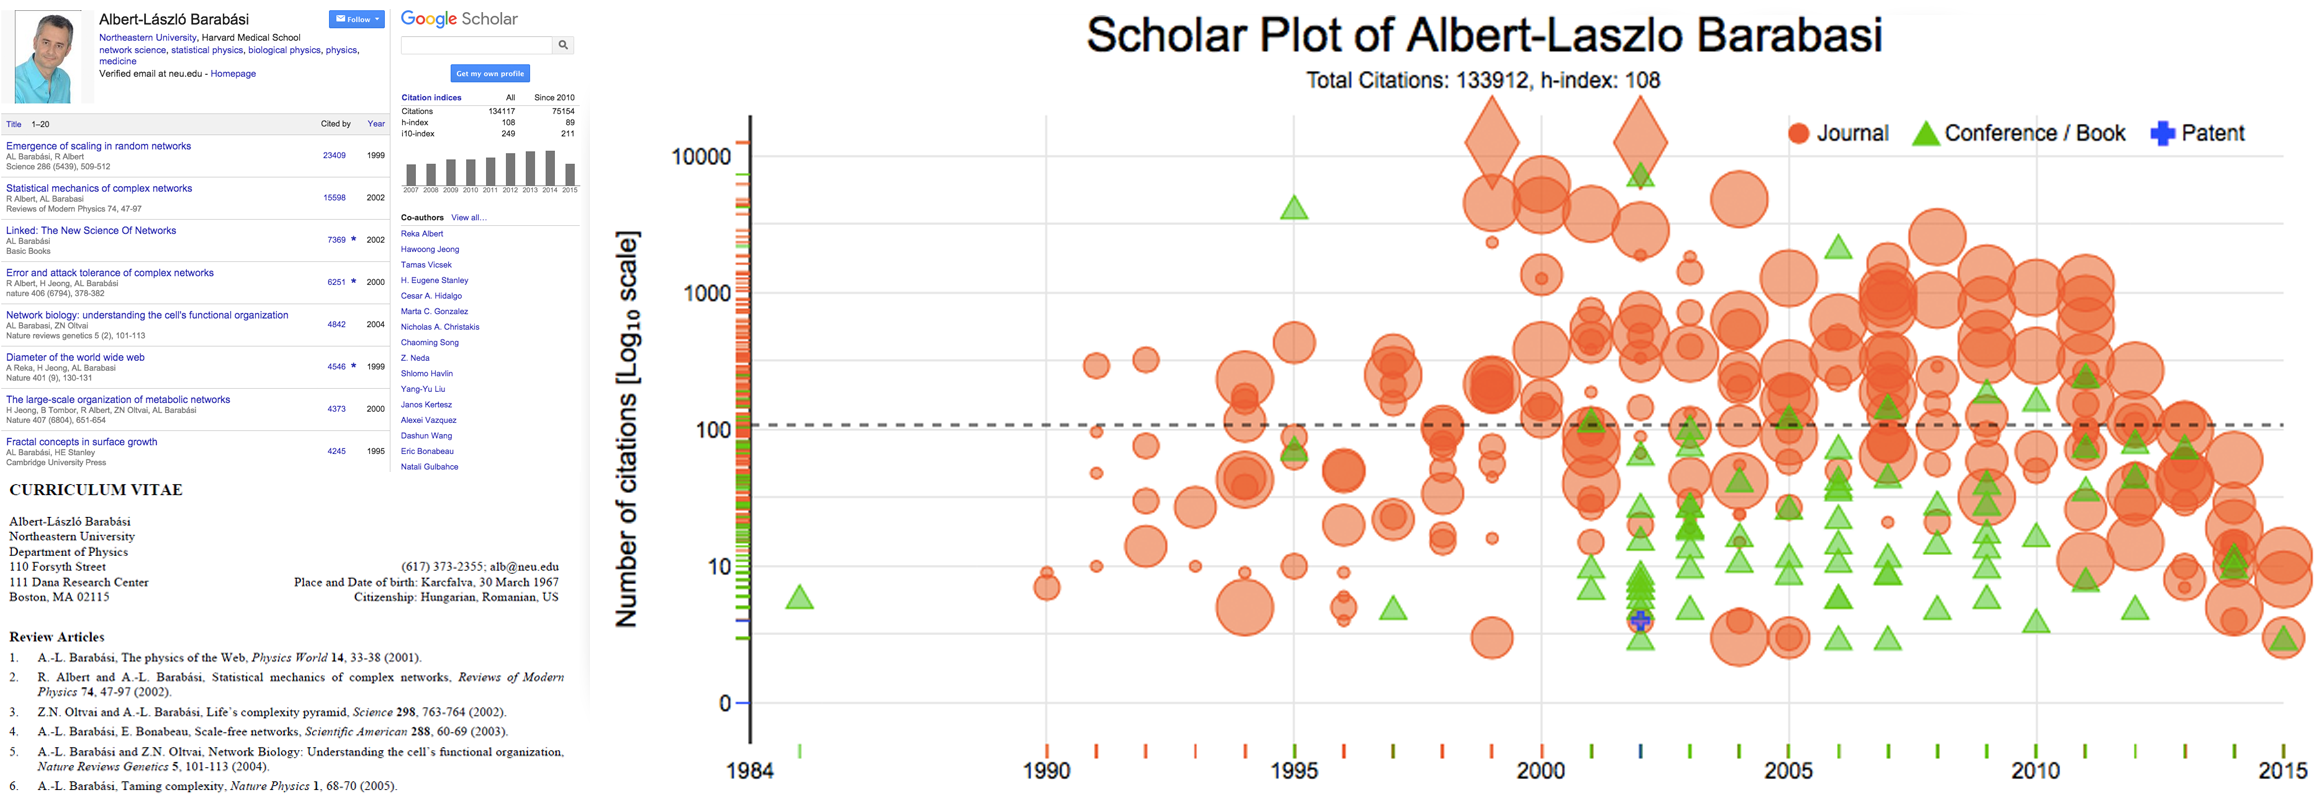
\includegraphics[width=1\columnwidth]{figures/fig_cv_google_scholarplot}
  \caption{An example of Scholar Plot - Visualizing Publication Data}~\label{fig:fig-publication}
 % \vspace{-1ex} 
\end{figure*}

Scholar Plot depicts the publications of an individual as a scatter plot and the NSF/NIH funding as a multiline plot. The publications are represented in a 2D diagram (number of citations vs. year of publication) with the {\it h}-index line (Figure \ref{fig:fig-publication}). The horizontal axis is time, starting with the year of the researcher's first publication ending with the current year. The vertical axis is the number of citations. The default plot is in $log_{10}$ scale. The user can also view the plot in the decimal scale by a toggle option using a radio button at the top left corner (Figure \ref{fig:fig-scale}). The log scale provides a standardized scale which helps to compare the plots of multiple scholars.



% --------------------------
\subsection{Visualizing Publication Data}
% --------------------------
Each publication $i$ is represented with a symbol. The center of the symbol has coordinates $(i_{PY}, i_{C})$, where $PY$ stands for Publication Year and $C$ for Number of citations obtained by the publication till date. The journals are represented as circles (orange) with area analogous to the impact factor the journal. The conferences / books are represented as triangles (green) and the patents as crosses (blue). By clicking at a symbol you can obtain the publication title, the year, the number of citations, the venue where published and its impact factor (if it is a journal), as well as a breakdown in the authorship, complete with the level of collaboration between the co-authors and the selected scholar (Figure \ref{fig:fig-tooltip}). The publication title also enables the user to navigate to the Google Scholar page for the selected paper. This helps to quickly verify and obtain further details of the selected publication. It makes user reach out to the PDF file directly if available. To enhance user experience, we customized the tooltip to give detailed information without overlapping the plots.

\begin{figure}[H]
\centering
  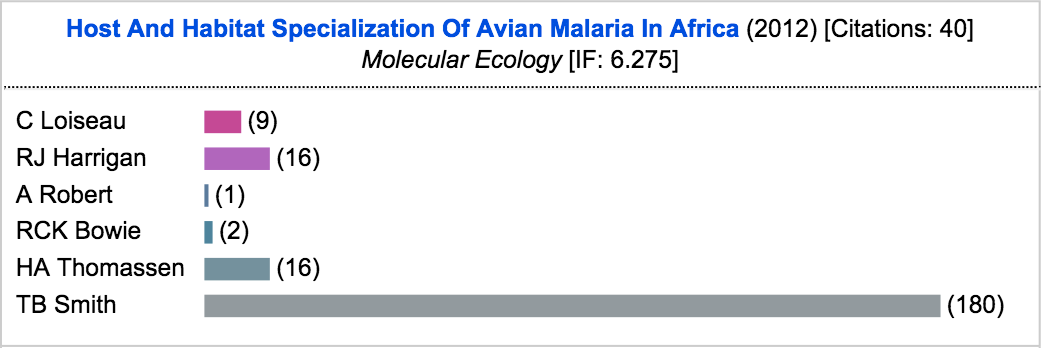
\includegraphics[width=1\columnwidth]{figures/fig_tooltip}
  \caption{An example of the tooltip: The publication title, the year, the number of citations, the venue where published, impact factor, the list of co-authors, the visual horizontal bars with the number of collaboration between the co-authors and the selected scholar.}~\label{fig:fig-tooltip}
 % \vspace{-1ex} 
\end{figure}

A dotted horizontal line on the plot denote the {\it h}-index of the scholar. We also denote those publications which earn greater than 10,000 citations with diamonds as they represent the great success in publications (Figure \ref{fig:fig-publication}). The title of the plot contains the name of the scholar and her/his total number of citations along with the {\it h}-index. At the top right corner of the plot, a legend shows the three different types of publications we distinctly display (Figure \ref{fig:fig-legend}).

\begin{figure}[!htb]
\centering
  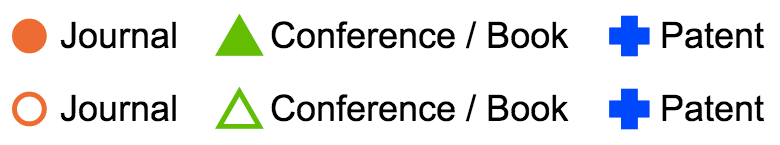
\includegraphics[width=0.9\columnwidth]{figures/fig_legend-toggle}
  \caption{The legend allows users to selectively view journals, conferences / books and patents.}~\label{fig:fig-legend}
 % \vspace{-1ex} 
\end{figure}

You can bring the journals, patents, and conferences / books in and out of the view by clicking at the respective legend. If there is an overlap between journals, conferences and patents, this feature can help the user to selectively view them. The user can also zoom into the plot for closer picture. Also note that the symbols are not completely opaque. So if there are multiple symbols which overlap, the user can see and interact with them by hovering the mouse over them appropriately.

% --------------------------
\subsection{Visualizing Funding Data}
% --------------------------
Scholar Plot also depicts the NSF/NIH funding of an individual as a multiline (Figure \ref{fig:funding}). Each breakpoint in the multiline corresponds to the individual's total amount in all NSF/NIH awards for the specific year. By pointing at a breakpoint you can obtain the NSF/NIH awards IDs, award amounts, and investigator's role. The total annual funding information per year is also available by clicking the legend. 

\begin{figure}[!htb]
  \centering
  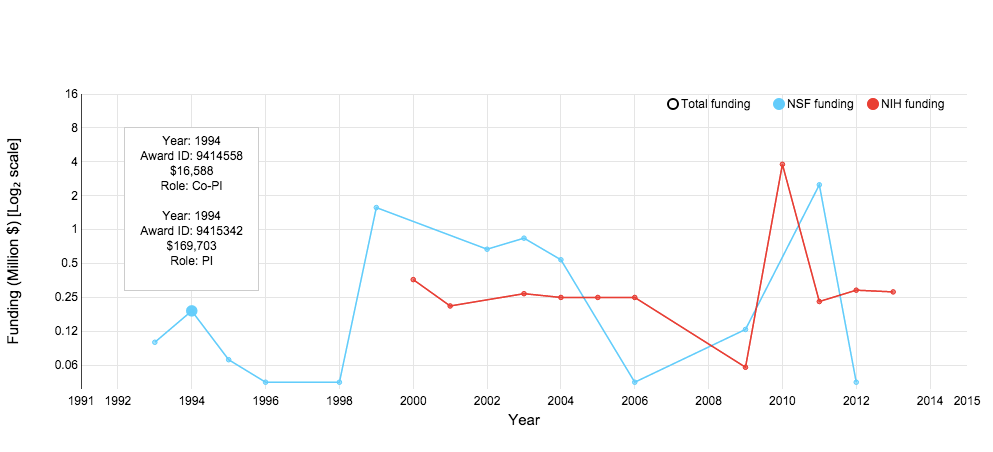
\includegraphics[width=1\columnwidth]{figures/fig_funding_default}
  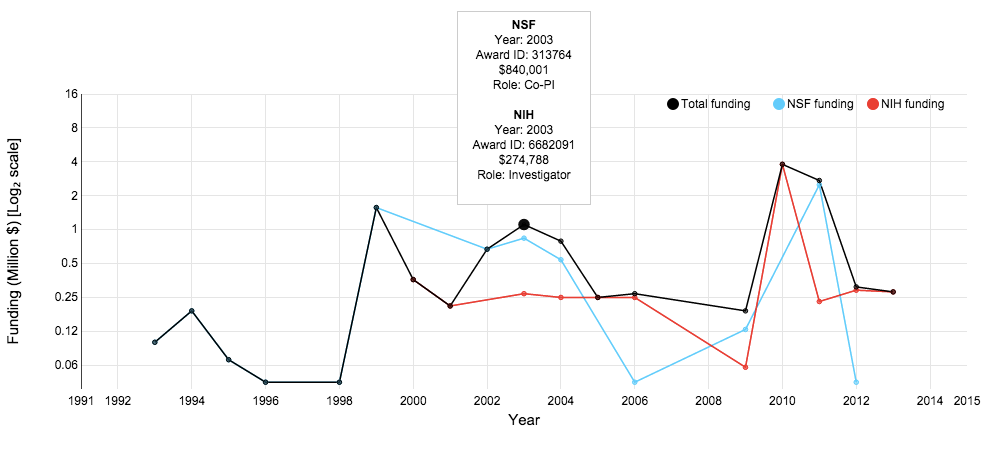
\includegraphics[width=1\columnwidth]{figures/fig_funding_total}
  \caption{An example of Scholar Plot - Visualizing Funding Data}~\label{fig:funding}
  % \vspace{-2ex} 
\end{figure}



%% --------------------------
%\subsection{Disk Size - How to determine the size of disks}
%% --------------------------
%We wanted to plot to visualize more efficiently with different size of disk for Journal publications that tells the different ranking of Journal by Impact Factor Index. To do this, we analyzed the data set of JCR 2013 IF and run quartile function as a useful concept in statistics to determine the size of disks in Scholar Plot. Based on this number, the system will decide the size of plot of each journal data and plot it in real-time. The quartile values are shown in table Table~\ref{tab:table1}. The maximum number from descriptive is 153.459 through. 
%
%\begin{table}
%  \centering
%  \begin{tabular}{c c}
%    \toprule
%    \multicolumn{2}{c}{\small{\textbf{ JCR Data (Impact Factor 2013) }}} \\
% 
%    {\small\textbf{Quartiles}}
%    & {\small \textit{IF}} \\
%    \midrule
%    Q1 & 0.67 \\
%    Q2 & 1.36 \\
%    Q3 & 2.47 \\
%    Q4 & 51.66 \\
%    \bottomrule
%  \end{tabular}
%  \caption{Table captions should be placed below the table. We
%    recommend table lines be 1 point, 25\% black. Minimize use of
%    unnecessary table lines.}~\label{tab:table1}
%\end{table}

%Scholar Plot gives a snapshot of the individuals profile in a concise manner.
To place the plots in your personal CV or on your web page we provide a download button at the top right corner of the plot (Figure \ref{fig:fig-scale}). This function enables the user to download plots in a zip file. It includes high resolution vector images in SVG (Scalable Vector Graphics) format of the publication and funding plots.

Scholar Plot also has a projection of the data on the y-axis depicted by small horizontal colored lines. For example, we can clearly see that journals contribute to the {\it h}-index of scholar in Figure \ref{fig:distribution} (a) and conferences / books contribute to the {\it h}-index of scholar in Figure \ref{fig:distribution} (b). We can clearly infer the scholar in Figure \ref{fig:distribution} (c)) has many patents. We can also infer the number of publications within a particular range of citations based on the density of the projected lines.

\begin{figure}[!htb]
\centering
\subfigure[]{%
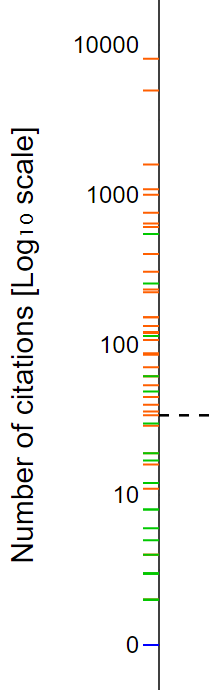
\includegraphics[width=0.23\columnwidth]{figures/fig_distribution_A}
}
\subfigure[]{%
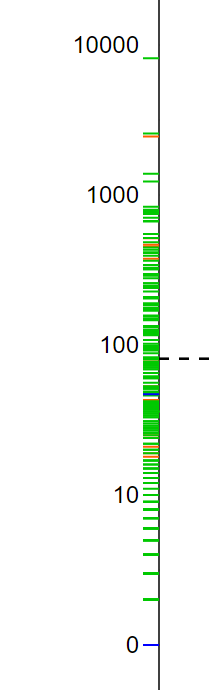
\includegraphics[width=0.23\columnwidth]{figures/fig_distribution_B}
}
\subfigure[]{%
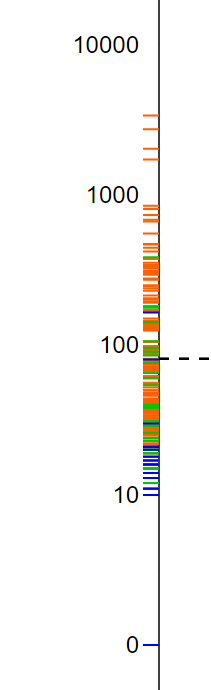
\includegraphics[width=0.23\columnwidth]{figures/fig_distribution_C}
}
\caption{Examples of y-axis projection for three different scholars.}~\label{fig:distribution}
  %\vspace{-1ex} 
\end{figure}

%\begin{figure}[!htb]
%  \centering
%  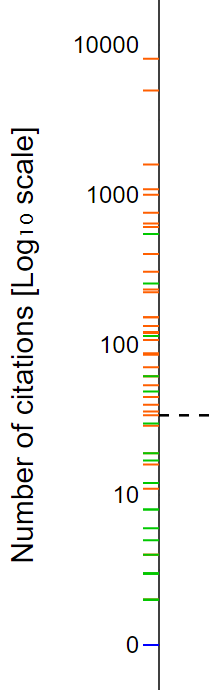
\includegraphics[width=0.2\columnwidth]{figures/fig_distribution_A}
%  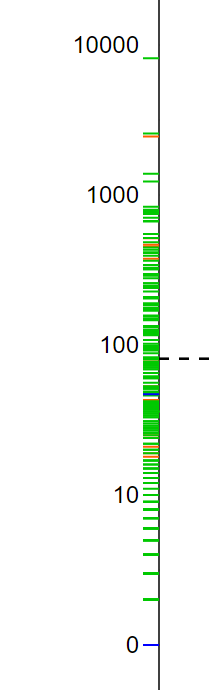
\includegraphics[width=0.2\columnwidth]{figures/fig_distribution_B}
%  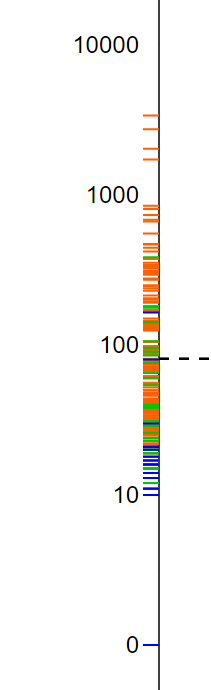
\includegraphics[width=0.2\columnwidth]{figures/fig_distribution_C}
%  \caption{Example with journals, conferences, and patents contributing to h-index}~\label{fig:distribution}
%\end{figure}

We improve user experience to enable users to quickly find and select from a pre-populated list of scholar names as they type. For each character the user enters, we display similar matching names on the dropdown list. Even entering the space (`` "), we display the 10 most recently inserted scholar's names. Scholar Plot follows the approach of responsive web design to provide optimal viewing based on the size of screen.


% =============================================================================
\section{System Architecture}
% =============================================================================
Scholar Plot is data visualization tool that uses HTML5, CSS3 and SVG to render a scholar's accomplishment at a glance. We created a MySQL database to store the mapping between the scholar names and their Google scholar IDs. We also designed and created database tables for NSF/NIH funding data. The user can search the name of the scholar in a text field. When the user starts to enter the name of the scholar, the names in our database which are similar to the entered name will be listed as a drop down list. We use jQuery and Ajax (asynchronous JavaScript and XML) method to have this feature, which connects to the database to get the list of names. If there are no matching/similar names, the user can also insert her/his Google Scholar ID to the database by one click event.

%Once the scholar's name selected, the user can run the application to see the visual results of the selected scholar's publications and fundings. Scholar Plot connects to the Web server to retrieve the necessary information.
The server-side application is implemented in PHP scripting language and MySQL. The HTTP protocol is used for communicating between client-side and server-side to get the basic information via JSON format (JavaScript Object Notation) and JSONP function (Figure \ref{fig:fig-arch}). Scholar Plot also uses htmlSQL library to parse Google scholar's page to extract user basic information \cite{htmlSQL}.
%, collecting for the publication title, the journal name, the co-authors' name, the year, and the citations. It also collects the {\it h-}index and the number of total citations from the top of the scholar's page up to 300 publications.

\begin{figure}
\centering
  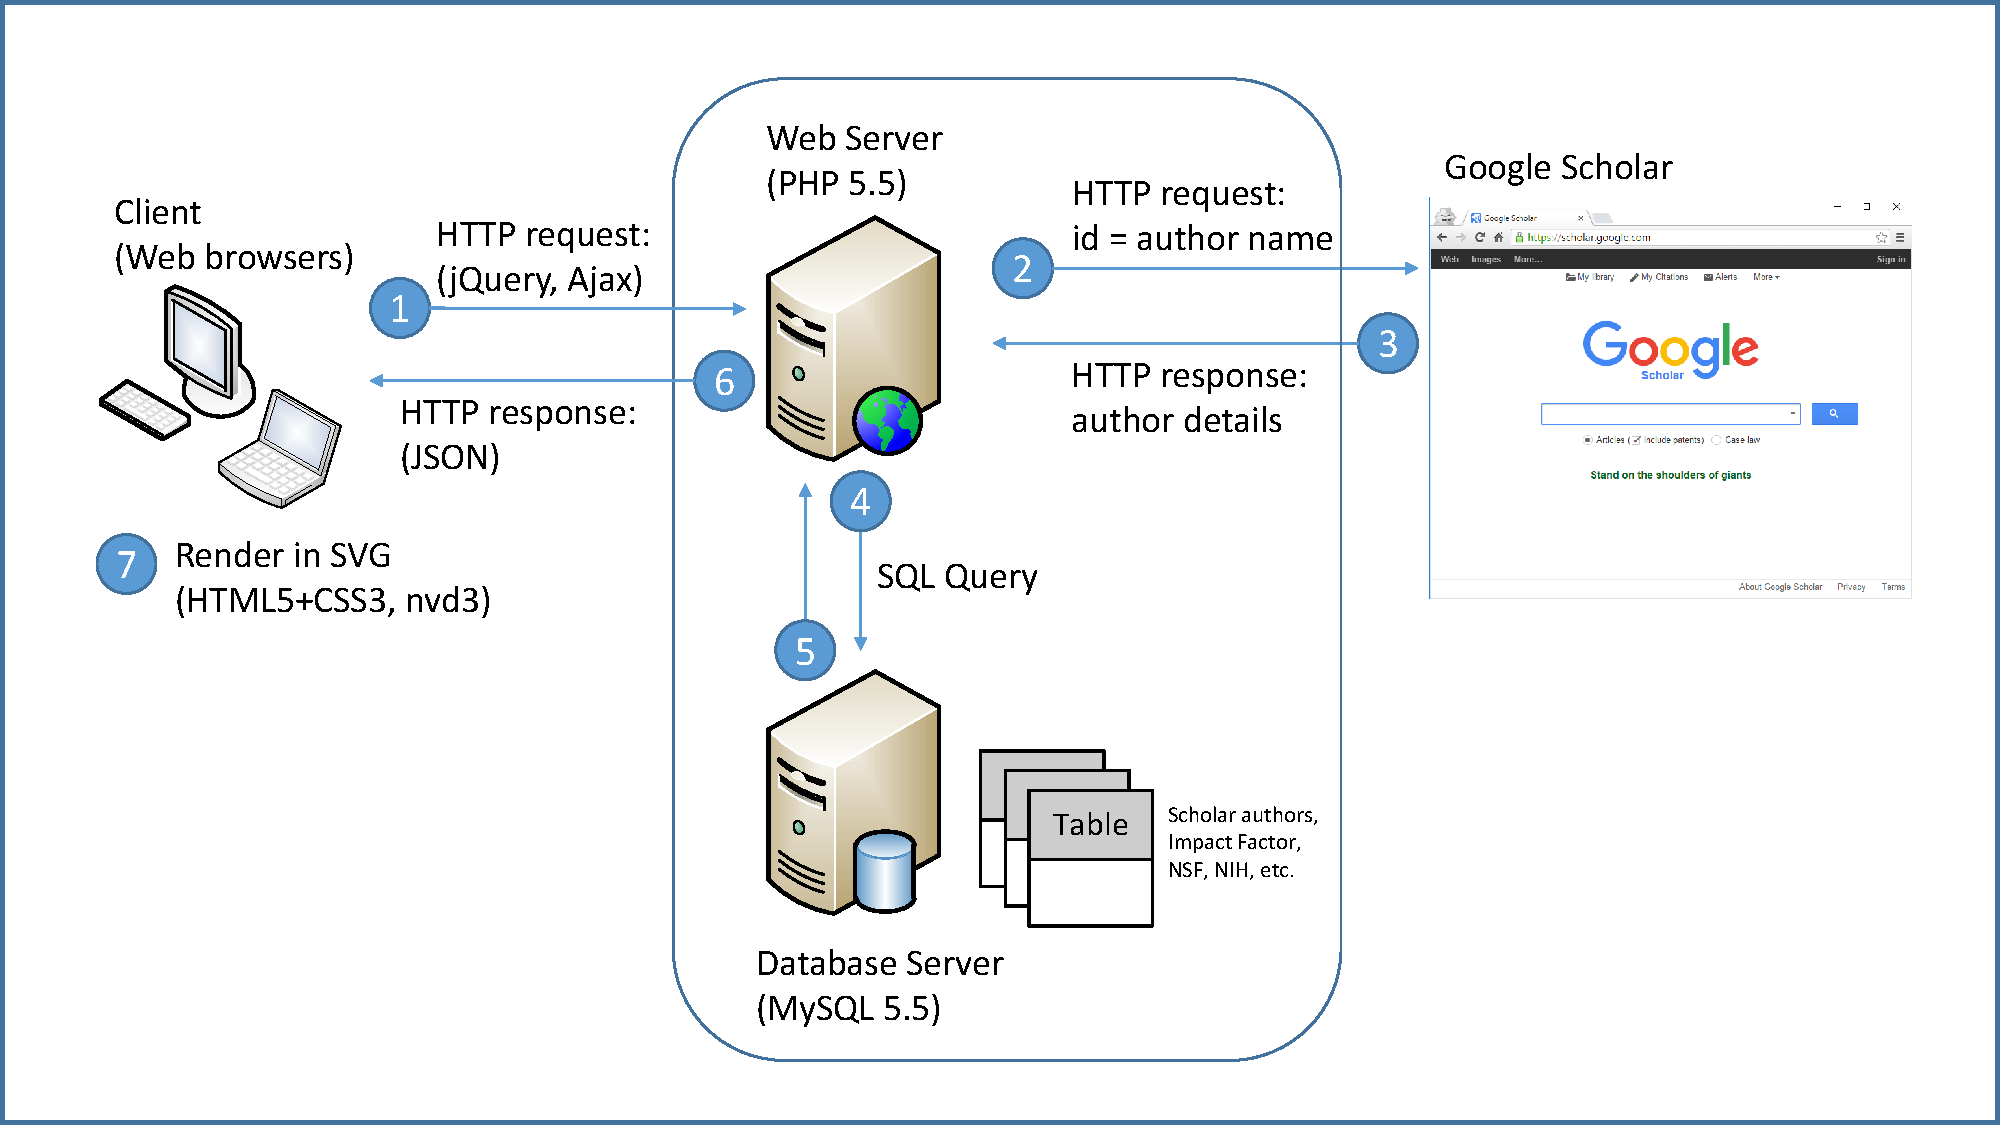
\includegraphics[width=1\columnwidth]{figures/fig_system_architecture.pdf}
  \caption{System Architecture of Scholar Plot.}~\label{fig:fig-arch}
%\vspace{-1ex} 
\end{figure}


% =============================================================================
\section{Name Disambiguation}
% =============================================================================
Google Scholar data has to be cleaned because it contains many non-english characters. We use regular expression to remove the invalid special characters and translate phonetic characters to english alphabets. We designed and implemented Algorithm \ref{alg:name} to match the author names in Google Scholar with those in NSF/NIH data. This process helps to improve the quality of results. 




% =============================================================================
\section{Name Disambiguation - Details}
\subsection{Within and across profile author name disambiguation}

Let $i$ be an index for the Google scholar profile researchers. Within each collaboration profile of $i$,  there are a set of $K_{0}$ raw name strings that you have extracted,  $Names_{k}$ indexed by $k_{i}$. We will use the fact that these strings are associated with profile $i$ in the process of name disambiguation across Google Scholar profiles. The following provides an outline of this procedure: \\


A) {\bf Clean last names:} 
Remove strings at end of all $Names_{k}$ that are not last names, and which may not consistently be listed for $k$, e.g. ``Jr.'', ``III'' etc. Hence, each name string  $Name_{k}$ consists ideally of a First name string $FN_{k}$, a Last name string $LN_{k}$, and possibly a Middle name string $MN_{k}$. \\

B)  {\bf Clean middle initial strings within each profile $i$:}  Within each $i$, search for inconsistencies in the use of $MN_{k}$. That is, possibly sometimes the author $k$ is listed as {\it Alexander M Petersen}, sometimes {\it Alexander Petersen}, and sometimes {\it Alexander Michael Petersen}. In this example the Last name string $LN_{k} = Petersen$ and the First name string $FN_{k} = Alexander$ are clearly consistent. But the Middle name string \{$\_$ , M, Michael\} causes some ambiguity if simple string comparison is used,  where $\_$ is a whitespace. 

%Hence, for each distinct  surname $FN_{k}$ and last name $LN_{k}$, map all $MN_{k}$ strings to the simplest representation $\hat X$ of just the middle name initials.\\

Then check to see how many different types of {\it Alexander} $\hat X$ {\it Petersen} occur within each $k$, where $\hat X$ is refers to the middle name. Use the following rules for when there are 2 or more types of $\hat W \hat X Petersen$.
 
 \begin{itemize}
 \item If there are only two  types of $Alexander \hat X Petersen$, with $\hat X=$ $\_$ or $M$, then map all of the $Alexander \hat X Petersen$ to $Alexander M Petersen$ for this $i$
 \item If there are only three types of $Alexander \hat X Petersen$, with $\hat X=$ starting with the same initial, $M\_$ or $M$, then map all of the $A\hat X Petersen$ to $Alexander Michael Petersen$ for this $i$
 \item If there are two or more types of $Alexander \hat X Petersen$, say $\hat X=O$ and $\hat X=P$, then keep these $X$ as they are.
 
%  \item However, if one of those types are a whitespace,  say $\hat X=O$ and $\hat X=P$  and $X= \_$, then we cannot know if the latter possibly corresponds to $O$ or $P$. This case shouldn't occur often. So we can use the simple heuristic that if there is any paper with $AO$ and $A$, then in this case the latter is actually $AP$, and so all $A\_$ are mapped to $AP$. If there are no papers that make obvious this distinction,  then compare the coauthors of $AO$ and $AP$  and $A \_$ within the profile of $i$. Map $A \_$ to $AP$ if they share more coauthors or map $A \_$ to $AP$ if they share more coauthors using the Jaccard Similarity measure to compare.
  
\end{itemize}

C)  {\bf Disambiguate coauthors $k$ across the Google Scholar profiles (connecting $i$):} Let  $k$ and $k'$ be coauthors in profiles $i$ and $i'$, respectively.   In this step we would like to identify $k$ and $k'$ that are likely the same person, $k=k'$, allowing us to connect the two profiles $i$ and $i'$ within the coauthor network.\\

 If $k$ and $k'$ have the same initials and same surname, then there is a possibility that they are the same individual. Also, if their full first name strings match, this is clearly very positive evidence of this. Let $A_{k,j}$ be the entire combination of First Name and Middle initial $FM_{k,j}$ with the surname $L_{k,j}$ (e.g. {\it Adam B Smith}, or {\it Adam \_ Johnson}) of the coauthor $j$ of the coauthor $k$. 

 \begin{itemize}
 \item If the full first name strings and the full last name strings are the same, $FN_{k,j}$=$FN_{k',j}$ and $LN_{k,j} = LN_{k',j}$ (e.g. Adam J. Johnson and Adam Johnson), and they both have at least one coauthors in common,  then they are considered the same coauthor. 
 \item If we don't have the added information of their full first names then we must rely more heavily on the information from their coauthors. If the first and last names are the same, $FM_{k,j}=FM_{k',j}$ and $LM_{k,j}=LM_{k',j}$, and there are more than 2 middle names with one of the middle name being empty, we do the following -
 
 We compute the number of coauthors in common of the empty middle name author with non-empty middle name authors by comparing the sets of coauthors, $\{j\}$.% and $\{j'\}$.
 
 We assign the empty middle name to that middle name for which there are more number of co-authors in common.
 
 \item If the first name of the author has a hyphen, we check for any other author having the same last name and the first name as the first word of the hyphenated word and middle name starting with the first letter of the second part of the hyphenated word. If any such pair of authors have at least one author in common, we update the first and middle name of the author with the hyphenated middle name to first name and middle name of the matched author.


\item If the first name of the author has only two letters, we check for any other author having the same last name and the first name starting with the first letter of the first name and middle name starting with the second letter of the first name. If any such pair of authors have at least one author in common, we update the first and middle names of the author with two letters to first and middle names of the matched author.
  
\end{itemize}
Google Scholar data has to be cleaned because it contains many non-english characters. We use regular expression to remove the invalid special characters and translate phonetic characters to english alphabets. We designed and implemented Algorithm \ref{alg:name} to match the author names in Google Scholar with those in NSF/NIH data. This process helps to improve the quality of results. 


%\input{chap3_Methods_AG.tex}
\chapter{Software Engineering and Algorithms}\label{chap:Algorithms}
% =============================================================================
\section{System Architecture}
% =============================================================================
Scholar Plot is data visualization tool that uses HTML5, CSS3 and SVG to render a scholar's accomplishment at a glance. We created a MySQL database to store the mapping between the scholar names and their Google scholar IDs. We also designed and created database tables for NSF/NIH/NASA funding data. The user can search the name of the scholar in a text field. When the user starts to enter the name of the scholar, the names in our database which are similar to the entered name will be listed as a drop down list. We use jQuery and Ajax (asynchronous JavaScript and XML) method to have this feature, which connects to the database to get the list of names. If there are no matching/similar names, the user can also insert her/his Google Scholar ID to the database by one click event.

%Once the scholar's name selected, the user can run the application to see the visual results of the selected scholar's publications and fundings. Scholar Plot connects to the Web server to retrieve the necessary information.
The server-side application is implemented in PHP scripting language and MySQL. The HTTP protocol is used for communicating between client-side and server-side to get the basic information via JSON format (JavaScript Object Notation) and JSONP function (Figure \ref{fig:fig-arch}). Scholar Plot also uses htmlSQL library to parse Google scholar's page to extract user basic information \cite{htmlSQL}.
%, collecting for the publication title, the journal name, the co-authors' name, the year, and the citations. It also collects the {\it h-}index and the number of total citations from the top of the scholar's page up to 300 publications.

\begin{figure}
\centering
  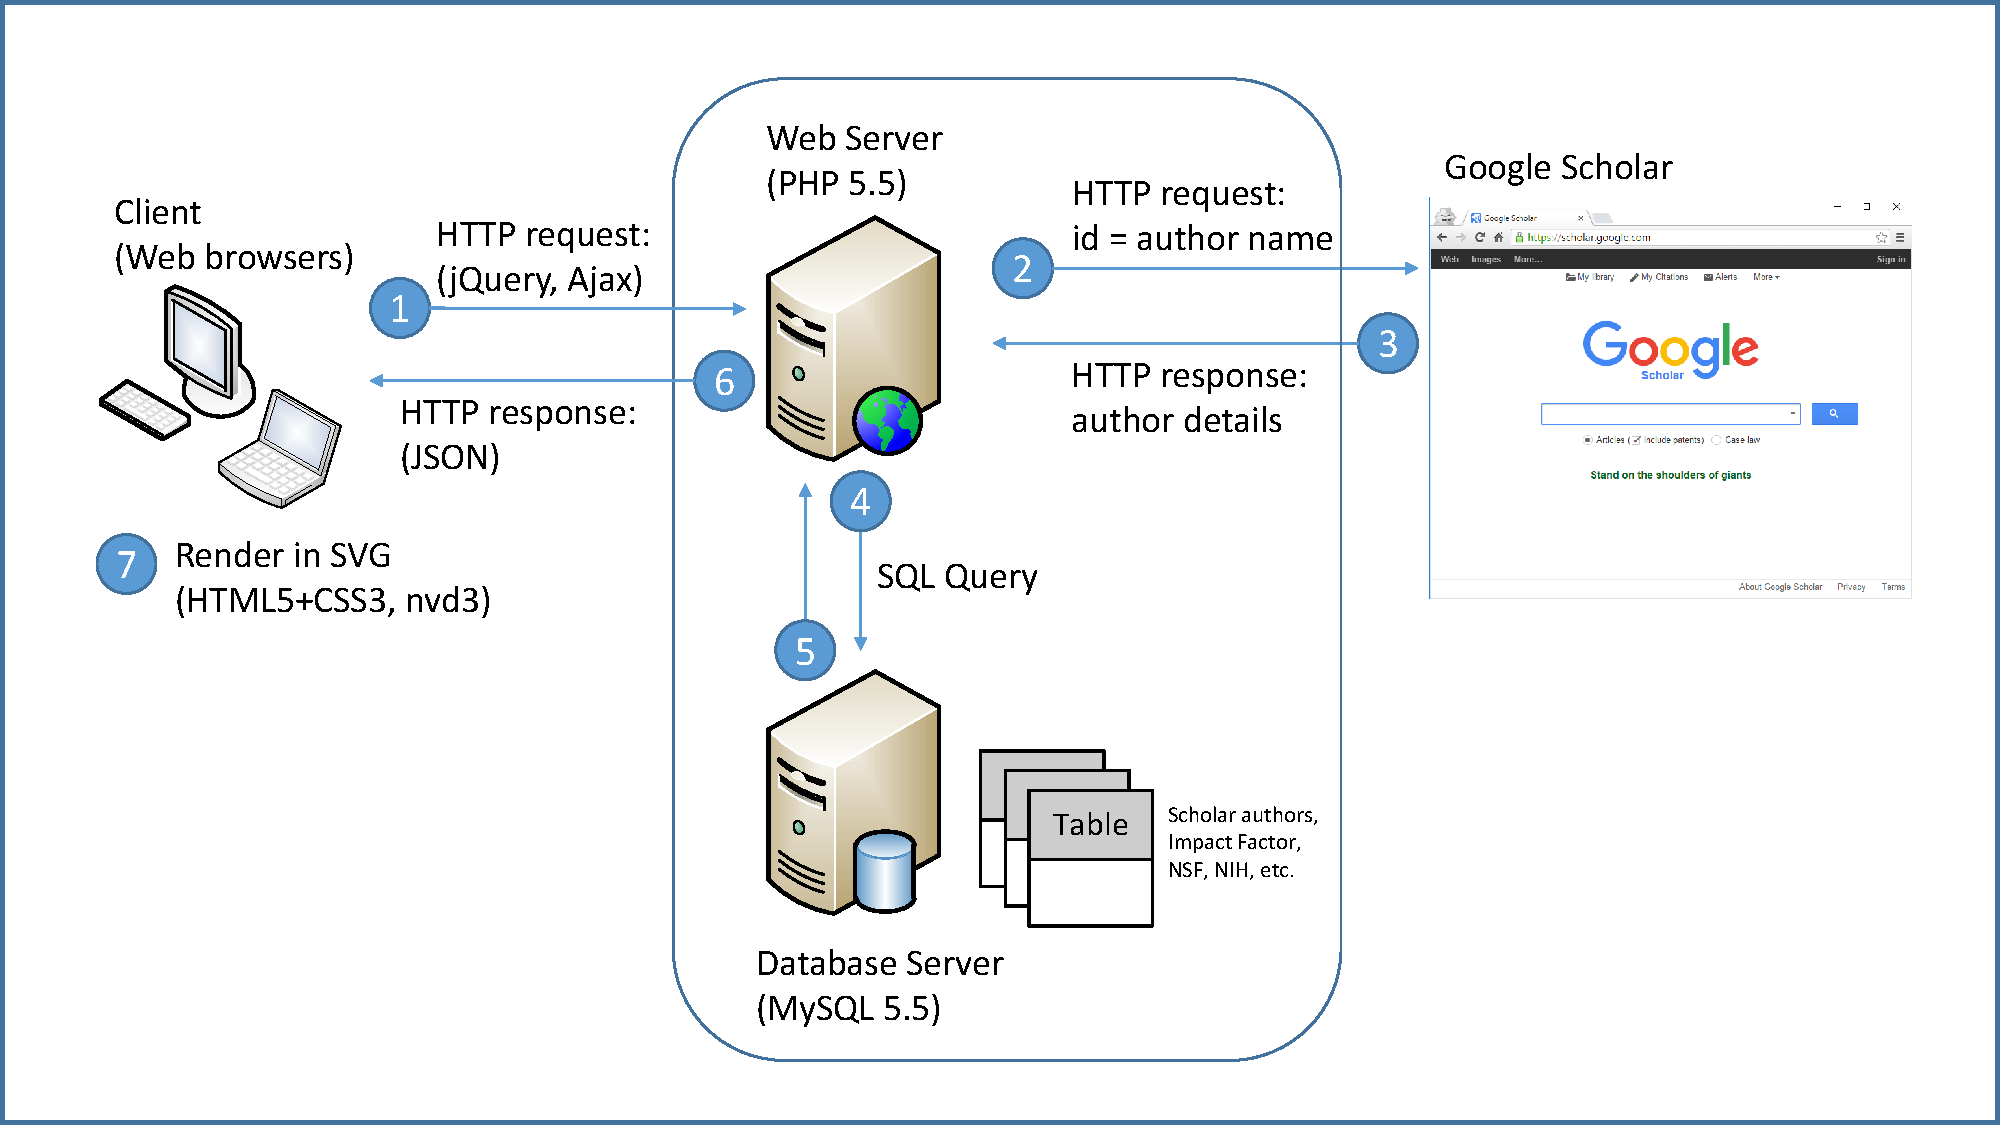
\includegraphics[width=1\columnwidth]{figures/fig_system_architecture.pdf}
  \caption{System Architecture of Scholar Plot.}~\label{fig:fig-arch}
%\vspace{-1ex} 
\end{figure}

The NSF/NIH/NASA funding datasets are available at the respective US government websites in various file formats such as XML, CSV and so on \cite{nsf, nih}. We implemented a script to parse this massive XML dataset into our data structure that consists of AwardID, AwardAmount, First name, Last name, Investigator by RoleCode (Principal Investigator, Co-Principal Investigator and Former Principal Investigator), using XMLStarlet \cite{XMLStarlet}. We imported this data to our database using Toad DBMS tool.

% =============================================================================
\section{Database Schema Diagrams}
% =============================================================================
\begin{figure}
\centering
  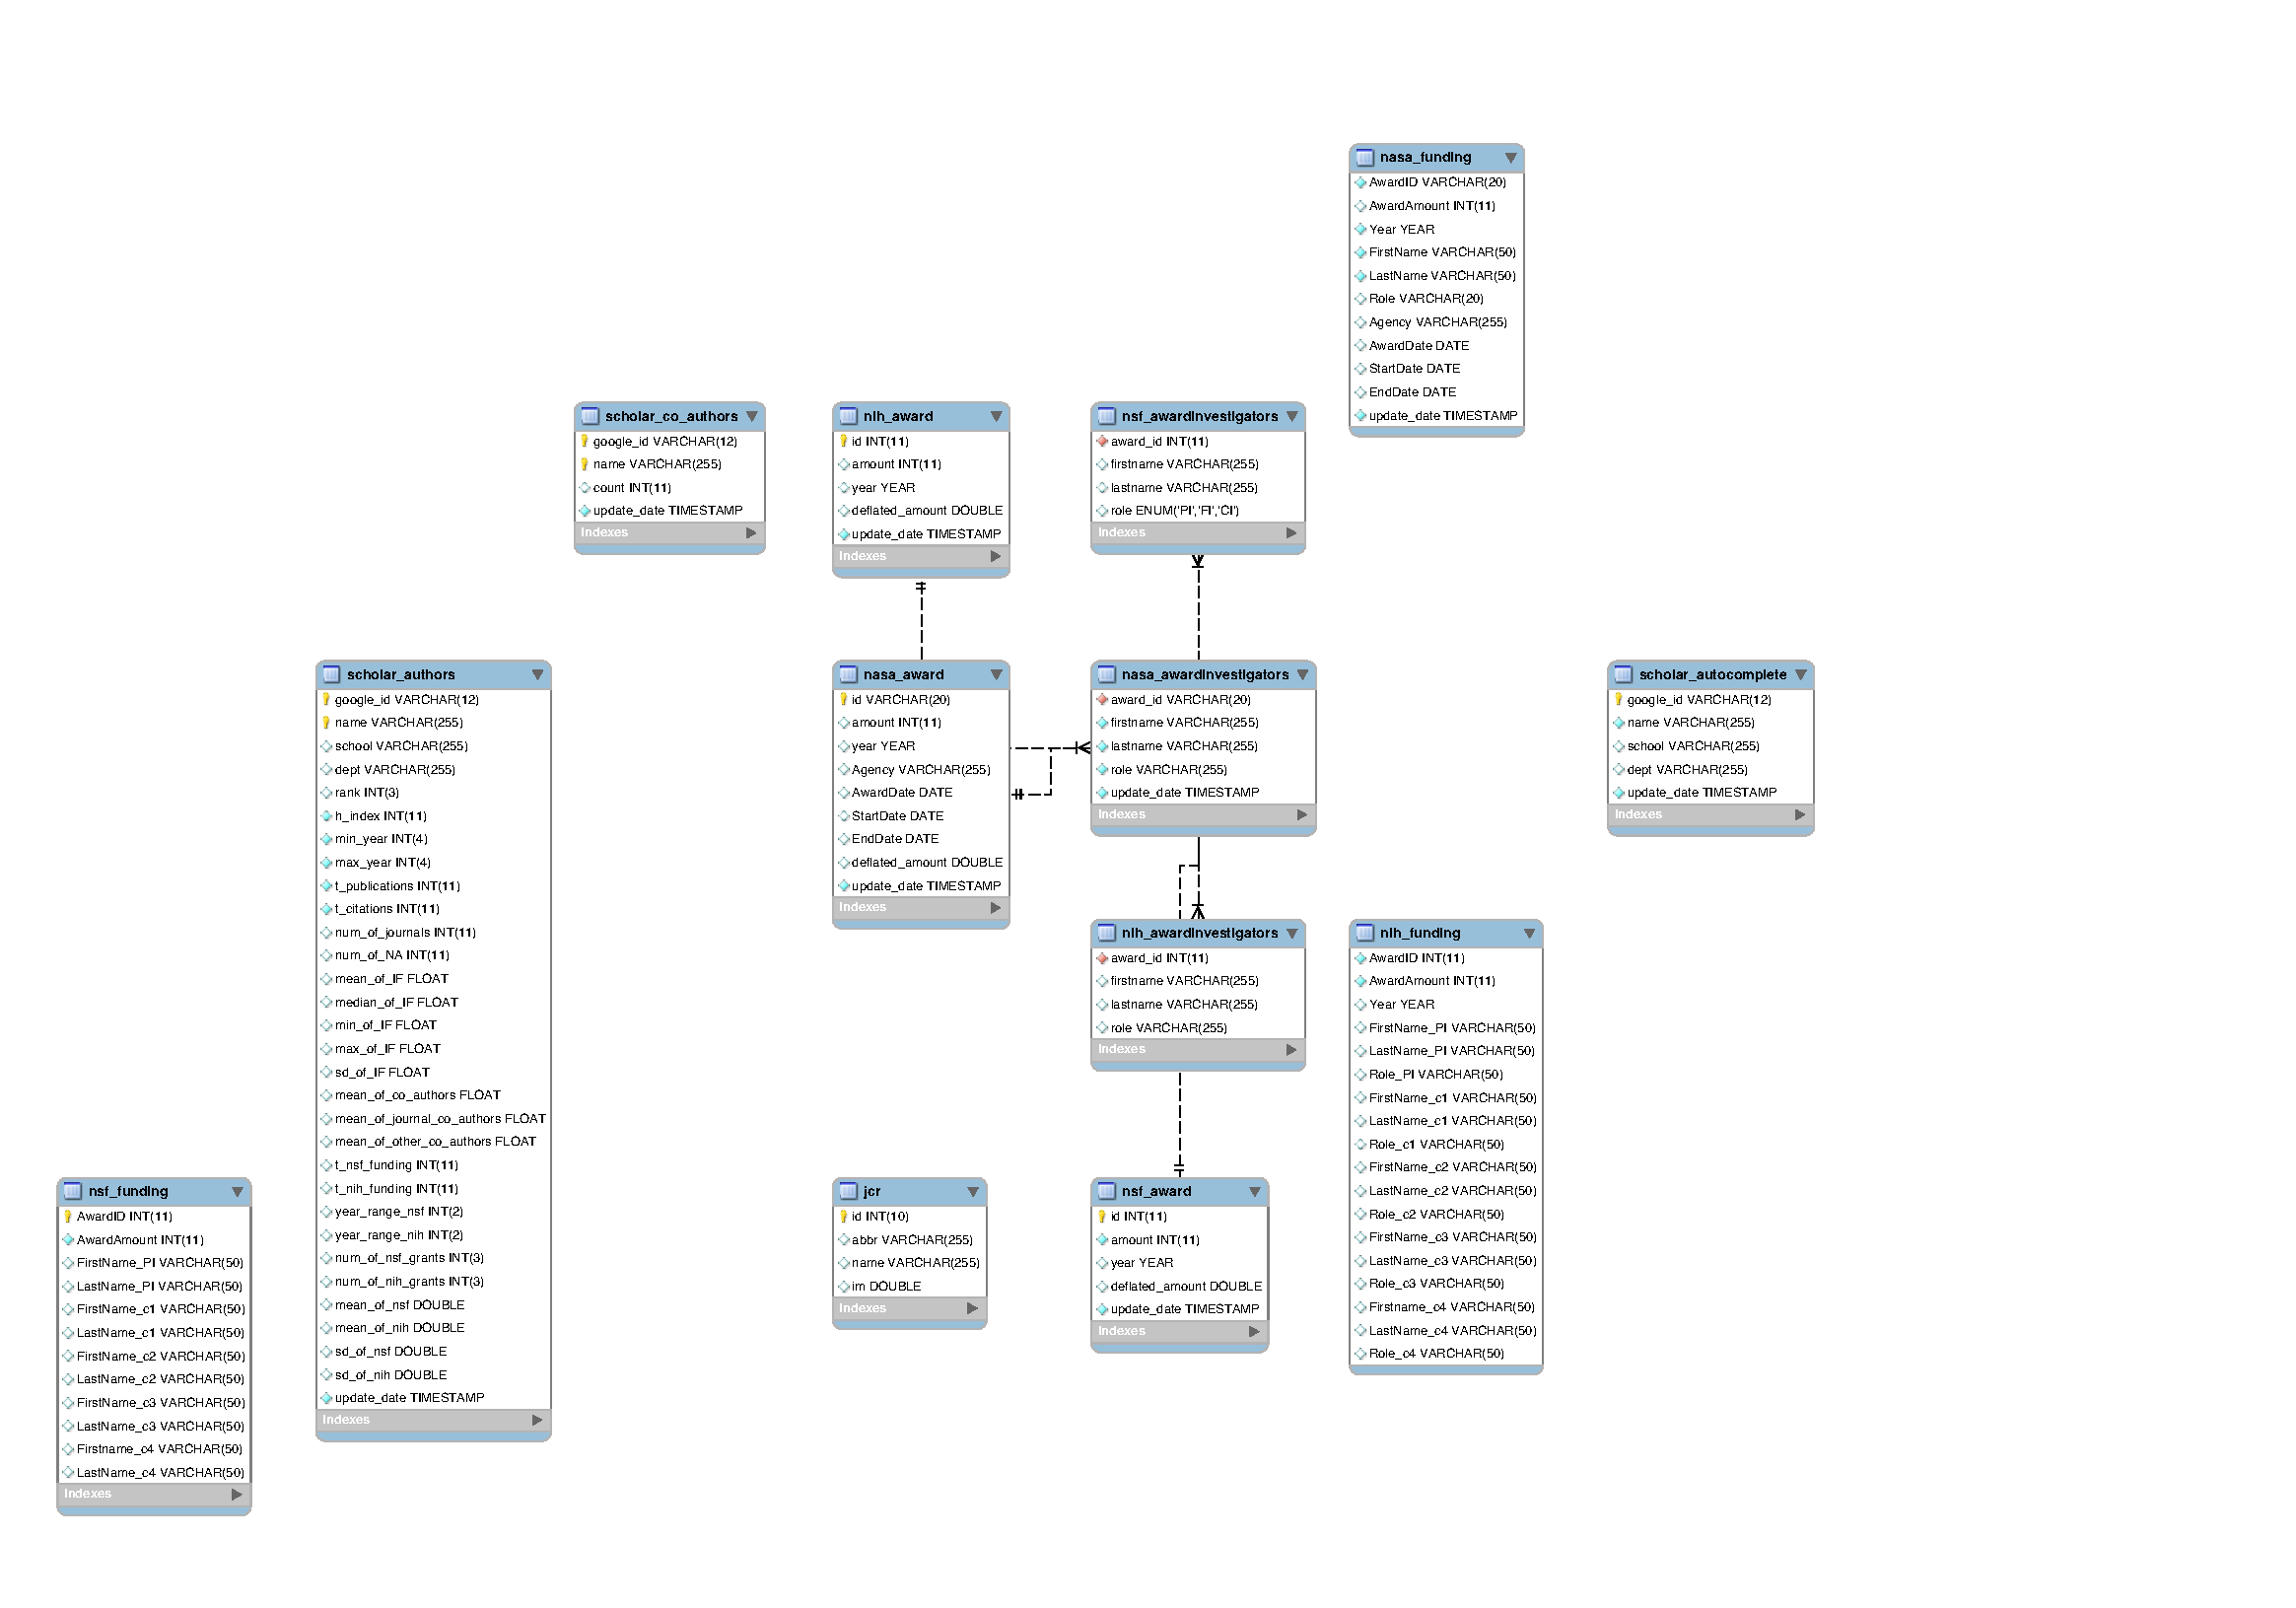
\includegraphics[width=1\columnwidth]{figures/fig_EER_Diagram.pdf}
  \caption{System Architecture of Scholar Plot.}~\label{fig:fig-arch}
%\vspace{-1ex} 
\end{figure}





% =============================================================================
\section{Name Disambiguation}
% =============================================================================
Google Scholar data has to be cleaned because it contains many non-english characters. We use regular expression to remove the invalid special characters and translate phonetic characters to english alphabets. We designed and implemented Algorithm to match the author names in Google Scholar with those in NSF/NIH/NASA data. This process helps to improve the quality of results. 




% =============================================================================
\section{Name Disambiguation - Details}
\subsection{Within and across profile author name disambiguation}

Let $i$ be an index for the Google scholar profile researchers. Within each collaboration profile of $i$,  there are a set of $K_{0}$ raw name strings that you have extracted,  $Names_{k}$ indexed by $k_{i}$. We will use the fact that these strings are associated with profile $i$ in the process of name disambiguation across Google Scholar profiles. The following provides an outline of this procedure: \\


A) {\bf Clean last names:} 
Remove strings at end of all $Names_{k}$ that are not last names, and which may not consistently be listed for $k$, e.g. ``Jr.'', ``III'' etc. Hence, each name string  $Name_{k}$ consists ideally of a First name string $FN_{k}$, a Last name string $LN_{k}$, and possibly a Middle name string $MN_{k}$. \\

B)  {\bf Clean middle initial strings within each profile $i$:}  Within each $i$, search for inconsistencies in the use of $MN_{k}$. That is, possibly sometimes the author $k$ is listed as {\it Alexander M Petersen}, sometimes {\it Alexander Petersen}, and sometimes {\it Alexander Michael Petersen}. In this example the Last name string $LN_{k} = Petersen$ and the First name string $FN_{k} = Alexander$ are clearly consistent. But the Middle name string \{$\_$ , M, Michael\} causes some ambiguity if simple string comparison is used,  where $\_$ is a whitespace. 

%Hence, for each distinct  surname $FN_{k}$ and last name $LN_{k}$, map all $MN_{k}$ strings to the simplest representation $\hat X$ of just the middle name initials.\\

Then check to see how many different types of {\it Alexander} $\hat X$ {\it Petersen} occur within each $k$, where $\hat X$ is refers to the middle name. Use the following rules for when there are 2 or more types of $\hat W \hat X Petersen$.
 
 \begin{itemize}
 \item If there are only two  types of $Alexander \hat X Petersen$, with $\hat X=$ $\_$ or $M$, then map all of the $Alexander \hat X Petersen$ to $Alexander M Petersen$ for this $i$
 \item If there are only three types of $Alexander \hat X Petersen$, with $\hat X=$ starting with the same initial, $M\_$ or $M$, then map all of the $A\hat X Petersen$ to $Alexander Michael Petersen$ for this $i$
 \item If there are two or more types of $Alexander \hat X Petersen$, say $\hat X=O$ and $\hat X=P$, then keep these $X$ as they are.
 
%  \item However, if one of those types are a whitespace,  say $\hat X=O$ and $\hat X=P$  and $X= \_$, then we cannot know if the latter possibly corresponds to $O$ or $P$. This case shouldn't occur often. So we can use the simple heuristic that if there is any paper with $AO$ and $A$, then in this case the latter is actually $AP$, and so all $A\_$ are mapped to $AP$. If there are no papers that make obvious this distinction,  then compare the coauthors of $AO$ and $AP$  and $A \_$ within the profile of $i$. Map $A \_$ to $AP$ if they share more coauthors or map $A \_$ to $AP$ if they share more coauthors using the Jaccard Similarity measure to compare.
  
\end{itemize}

C)  {\bf Disambiguate coauthors $k$ across the Google Scholar profiles (connecting $i$):} Let  $k$ and $k'$ be coauthors in profiles $i$ and $i'$, respectively.   In this step we would like to identify $k$ and $k'$ that are likely the same person, $k=k'$, allowing us to connect the two profiles $i$ and $i'$ within the coauthor network.\\

 If $k$ and $k'$ have the same initials and same surname, then there is a possibility that they are the same individual. Also, if their full first name strings match, this is clearly very positive evidence of this. Let $A_{k,j}$ be the entire combination of First Name and Middle initial $FM_{k,j}$ with the surname $L_{k,j}$ (e.g. {\it Adam B Smith}, or {\it Adam \_ Johnson}) of the coauthor $j$ of the coauthor $k$. 

 \begin{itemize}
 \item If the full first name strings and the full last name strings are the same, $FN_{k,j}$=$FN_{k',j}$ and $LN_{k,j} = LN_{k',j}$ (e.g. Adam J. Johnson and Adam Johnson), and they both have at least one coauthors in common,  then they are considered the same coauthor. 
 \item If we don't have the added information of their full first names then we must rely more heavily on the information from their coauthors. If the first and last names are the same, $FM_{k,j}=FM_{k',j}$ and $LM_{k,j}=LM_{k',j}$, and there are more than 2 middle names with one of the middle name being empty, we do the following -
 
 We compute the number of coauthors in common of the empty middle name author with non-empty middle name authors by comparing the sets of coauthors, $\{j\}$.% and $\{j'\}$.
 
 We assign the empty middle name to that middle name for which there are more number of co-authors in common.
 
 \item If the first name of the author has a hyphen, we check for any other author having the same last name and the first name as the first word of the hyphenated word and middle name starting with the first letter of the second part of the hyphenated word. If any such pair of authors have at least one author in common, we update the first and middle name of the author with the hyphenated middle name to first name and middle name of the matched author.


\item If the first name of the author has only two letters, we check for any other author having the same last name and the first name starting with the first letter of the first name and middle name starting with the second letter of the first name. If any such pair of authors have at least one author in common, we update the first and middle names of the author with two letters to first and middle names of the matched author.
  
\end{itemize}
Google Scholar data has to be cleaned because it contains many non-english characters. We use regular expression to remove the invalid special characters and translate phonetic characters to english alphabets. We designed and implemented Algorithm \ref{alg:name} to match the author names in Google Scholar with those in NSF/NIH/NASA data. This process helps to improve the quality of results. 


%% =============================================================================
%\section{Scholar Plot Design - Base Level}
%% =============================================================================
%The base level of Scholar Plot (SP) visualizes individual academic records. The first issue we had to address as part of the design process for this level was to determine what to visualize. To answer this question we looked at the merit criteria considered by promotion, tenure, and search committees; these are: a) publication quality and quantity, and b) research funding. Furthermore, publication quality is defined by two factors: citation counts and prestige of the journals where the publications appeared. 
%
%Accordingly, we decided to structure individual scholar plots as two-panel arrangements - the top panel visualizing the individual's publication record, while the bottom panel visualizing the individual's research funding record (Fig. \ref{fig:ScholarPlot}). This arrangement brings to the fore any causal relationship that may exist between funding and publishing, as publication production is often powered by research dollars. The common timeline in the horizontal axes of the two panel graphs facilitates such an association. 
%
%\begin{figure*}
%%  \begin{minipage}{\columnwidth}
%    \centering
%    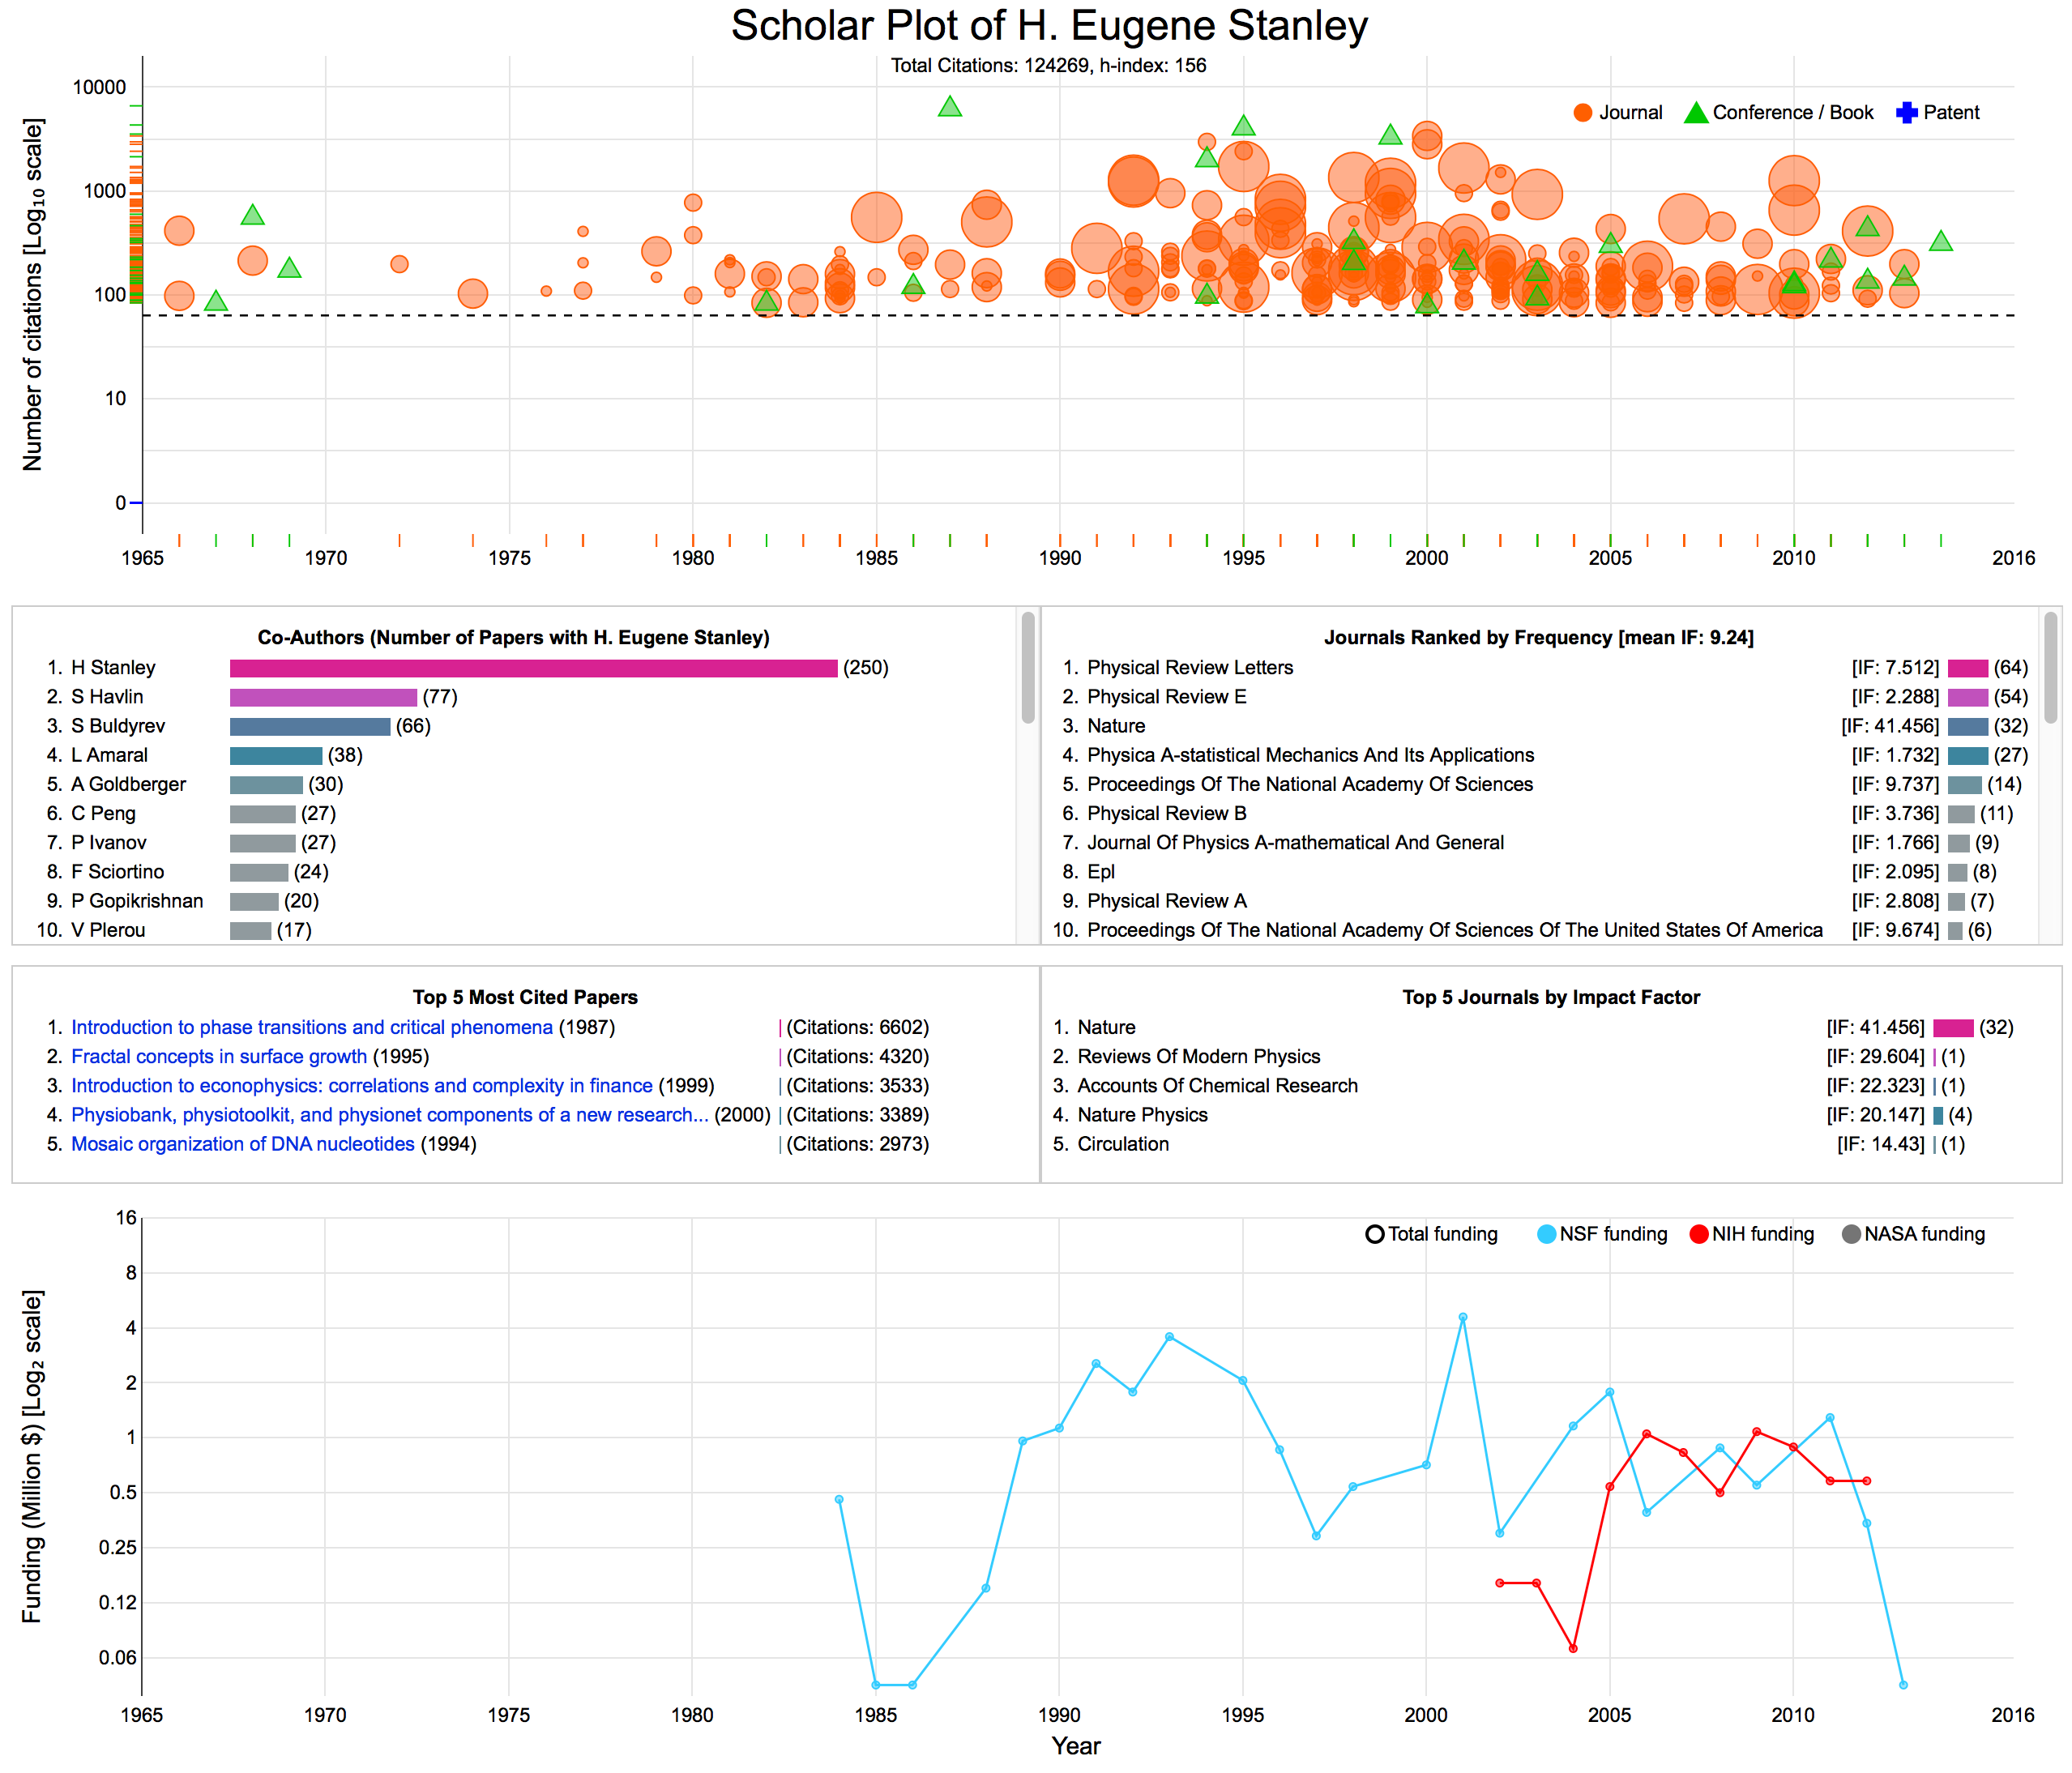
\includegraphics[width=1\textwidth]{figures/fig-EugeneStanley}
%    \caption{Base level Scholar Plot (SP) example - a famous physicist and interdisciplinary scientist with dozen of articles in \emph{Nature}. The summary panels in the middle were added after feedback from the focus group. Notice how this scholar's publication production exploded in sync with the commencement of substantial federal funding.}~\label{fig:ScholarPlot} 
%%    \end{minipage}
%\end{figure*} 
%
%The vertical axis of the publication graph indexes citation counts (Fig. \ref{fig:ScholarPlot}) - an important quality indicator for a publication. As we mentioned, the prestige of the publication venue is another important quality indicator. We convey this additional measurement dimension by varying the size of the graph points. 
%
%Only journals have a widely accepted ranking system reflecting prestige - the Journal Impact Factor (IF) List, issued every year by Thomson Reuters. Hence, we opted to represent different publication types with different symbols,  varying the symbol size of  journal publications only, for which an established ranking system exists. We chose disks to be the symbols of journal publications, as disk scaling can be done very effectively by simply varying its radius ($A \sim r^2$). Specifically, after performing histogram analysis on the IFs of journal publications, we settled on four disk sizes to represent journal prestige: $\#1 < \#2 < \#3 < \#4$ (Fig. \ref{fig:symbols}). We found that the great majority of journal publications appear in journals with $\mbox{IF} < 2$, assigning to this cohort the smallest disk size symbol, $\# 1$.  These are mid-level specialized technical and scientific journals. The next IF bracket  ($2 \leq \mbox{IF} < 4$) includes high quality specialized technical (e.g., IEEE Transactions) and scientific journals represented by disk \#2. The third IF bracket ($4 \leq \mbox{IF} < 16$) includes  very high quality science journals and specialized medical journals represented by disk  \#3. The top IF bracket ($\mbox{IF} \geq 16$) includes famous general science journals (e.g., \emph{Nature}) and top medical journals (e.g., \emph{New England Journal of Medicine}); they are assigned the largest disk, $\#4$.
%
%In the funding graph, each funding agency is represented by a polyline with a characteristic color (Fig. \ref{fig:ScholarPlot}). Grants are reported at the year they were awarded. If more than one grant was awarded by the same agency the same year to the specific investigator, then the full list shows up by rolling the mouse over the corresponding point in the polyline.
%
%The end effect of this simple visualization scheme is a picture that does not only compress dozens of CV pages, but also brings to the fore nuanced information about an academic's profile that can be grasped at a glance. Here are some examples:
%\begin{figure*}
%%  \begin{minipage}{\columnwidth}
%    \centering
%    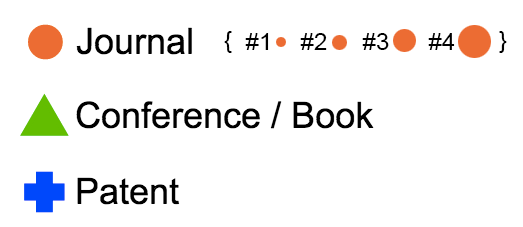
\includegraphics[width=0.5\textwidth]{figures/fig-disksize}
%    \caption{Publication symbols.}
%    \label{fig:symbols} 
%%    \end{minipage}
%\end{figure*}
%\begin{enumerate}
%\item It is easy to identify what type of publication powers the individual's scholarship - a correlate of disciplinary culture. For example, it is easy to spot career profiles of computer scientists and engineers (Fig. \ref{fig:Splots}a), where typically scholarship is built on conference rather than journal publications.
%\item It is easy to identify if the individual's scholarship is heavily associated with high or mid/low IF journals. If the publication graph is full of mid or small disks, this indicates that the scholar has done prolific methodological work that appeared in good specialized journals (Fig. \ref{fig:Splots}b). If the publication graph is full of large disks, this indicates that the scholar has done trendy and novel work that appeared in famous journals (Fig. \ref{fig:Splots}c).
%\item It is easy to identify if high funding levels yield high quantity and quality of publications or not (Fig. \ref{fig:ScholarPlot}). This may be especially useful to NSF and NIH reviewers who assess among other things the quality and impact of the investigator's prior work for the funding amounts s/he received.
%\begin{figure*}
%    \centering
%    \subfigure[SP of an accomplished Engineer.]{%
%    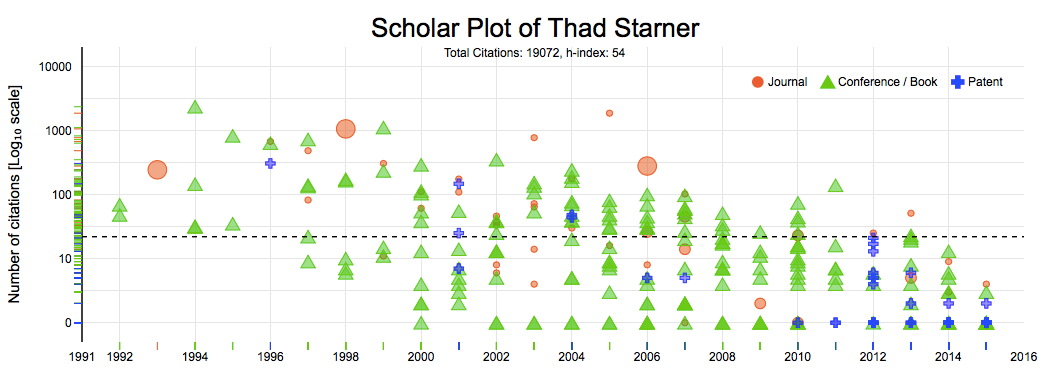
\includegraphics[width=1.0\textwidth]{figures/fig-ThadStarner}
%    } \\
%    \subfigure[SP of an accomplished Physicist.]{%
%     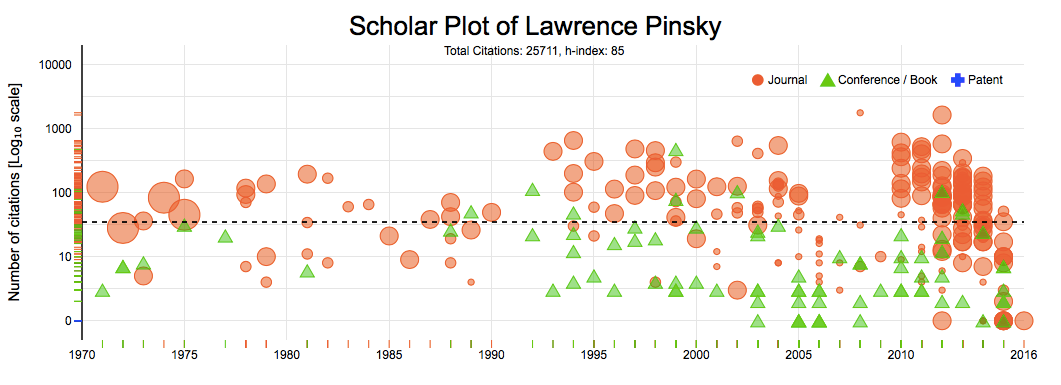
\includegraphics[width=1.0\textwidth]{figures/fig-LawrencePinsky}
%     }\\
%      \subfigure[SP of a famous Interdisciplinarian.]{%
%     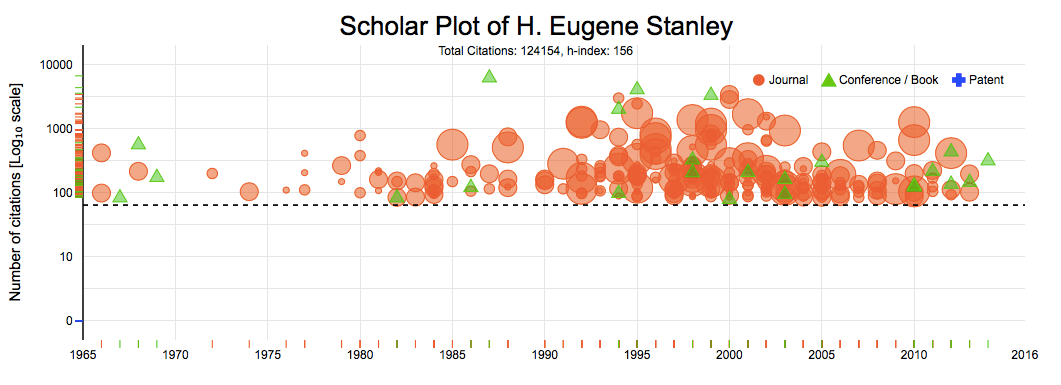
\includegraphics[width=1.0\textwidth]{figures/fig-EugeneStanley-pub}
%     }
%     \caption{}~\label{fig:Splots} 
%\end{figure*} 
%\end{enumerate}
%
%% =============================================================================
%\section{Scholar Plot Data Sources}
%% =============================================================================
%There were several options to get bibliographic data for powering the publication graph of Scholar Plot (SP). These included \href{http://www.scopus.com/}{Scopus}, \href{http://www.isiknowledge.com/}{ISI Web of Knowledge}, and \href{http://scholar.google.com}{Google Scholar}. We chose Google Scholar for two reasons: a) it is all inclusive, covering all types of publications, that is, journals, conferences, books, and patents; and, b) it is freely available.
%
%Our choice carries a few challenges, too. Google Scholar does not provide an application programming interface. Hence, we had to develop elaborate software to scrape information off publicly available Google Scholar pages. Also, not every academic has a Google Scholar page. This has been changing fast, however, as one college after the other in the United States mandating their faculty to maintain a Google Scholar page. 
%
%We use the Journal IF List issued every year by Thompson Reuters to assign disk sizes to journal publications.
%
%For funding records, we use the publicly available grant records from the \href{http://www.nsf.gov/awardsearch/download.jsp}{National Science Foundation (NSF)}, the \href{http://exporter.nih.gov/ExPORTER_Catalog.aspx}{National Institutes of Health (NIH)}, and the \href{https://www.research.gov/research-portal/appmanager/base/desktop?_nfpb=true&_eventName=viewQuickSearchFormEvent_so_rsr}{National Aeronautics and Space Administration (NASA)}. These are the only funding agencies with publicly available datasets at this point.

% ==================================================
\chapter{Results}\label{chap:Results}
% ==================================================

% --------------------------
\section{User Feedback - Usability Study}
% --------------------------



A total of 15 participants from various disciplines including Natural Sciences, Social Sciences, Life Sciences, and Computer Science evaluated Scholar Plot. We asked each participant to review the interface and complete an online survey. Special care was taken to ensure that the participants had correct understanding about the visualization component before they began rating. The participants answered the questions on a Likert scale from 1 to 5 with 1 being strongly disagree and 5 being strongly agree.

Figure \ref{fig:UserStudy} illustrates the mean evaluation for each visualization component. Accuracy, usability, and understandability of Scholar Plot scored the highest $(\mu = 4.2)$ as it is very intuitive and can be used with minimal assistance. The highest positive feedback we received from many of the participants was the visual scheme of Scholar Plot. Another observation is that the participants agree to use Scholar Plot to evaluate themselves $(\mu = 4.1)$. They suggested that Scholar Plot can be improved by adding more funding agencies. Overall, this evaluation indicated that Scholar Plot is a user-friendly tool that complements the CV which can be used to review a scholar's accomplishments. The survey has been approved by the University of Houston Institutional Review Board (IRB).

 \begin{figure}[!htb]
  \centering
  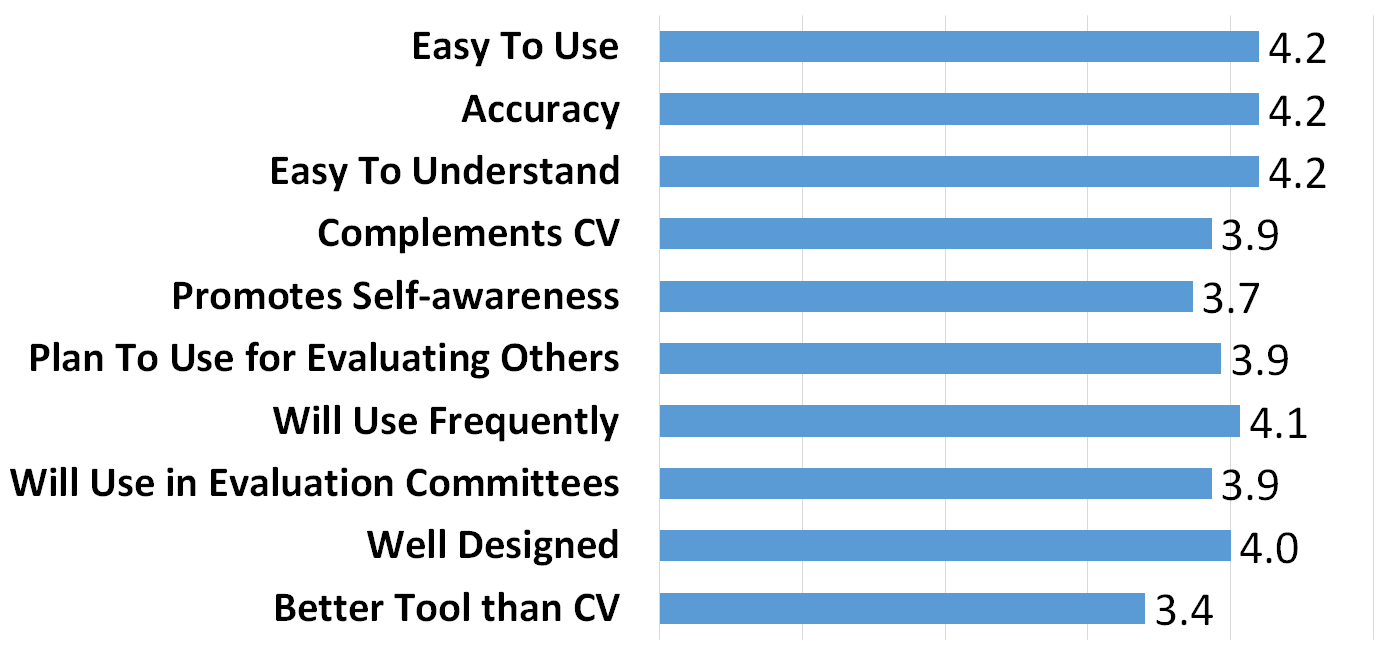
\includegraphics[width=\textwidth]{figures/fig_survey_chart}
%  \vspace{-3ex}
  \caption{Mean evaluation of Scholar Plot. A total of $n=15$ participants evaluated the survey.}
  \label{fig:UserStudy}
\end{figure}



% --------------------------
\section{User Feedback - Focus Group}
% --------------------------

We ran a focus group with 10 Principal Investigators and their post doctoral students at Northwestern University. The participant set included biologists, physicists, computer scientists, and social scientists. The focus group's suggestions are synopsized as follows:
\begin{description}
\item [Interface team science information.] Participants wanted to see the number and intensity of collaborations for the depicted scholar.
\item [Summarize highly cited papers.] Participants wanted to see explicitly in a side panel the scholar's most popular papers.
\item [Interface journal profile.] Participants wanted to see the specific journals where the scholar publishes most often and their impact factors.
\end{description}

The participants believed that accessorizing the central publication graph with this additional information would support deeper instant comprehension without compromising the elegance of Scholar Plot's compact visual representation. Specifically, this additional interface would reveal the collaborative nature of the scholar's work, give hints if s/he is a regular in specific disciplinary journals or if publishes in a variety of journals (interdisciplinarity), and give the rank of these journals. % All this information can also be gleaned by rolling the mouse over the publication graph, reading the tooltips, and summarizing it in panels under the graph. However, renders such manual investigation unnecessary.

\begin{figure}[H]
    \centering
    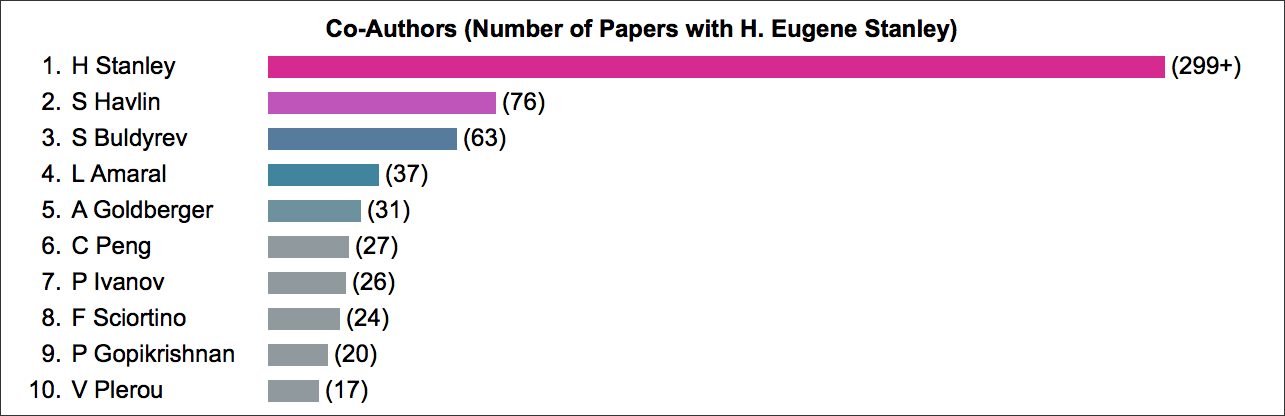
\includegraphics[width=\textwidth]{figures/fig_panel1-N}
    \caption{Panel listing the top collaborators with the selected scholar ranked by the count of the number of publications collaborated.}
    \label{fig:panel1}
\end{figure}

\begin{figure}[H]
    \centering
    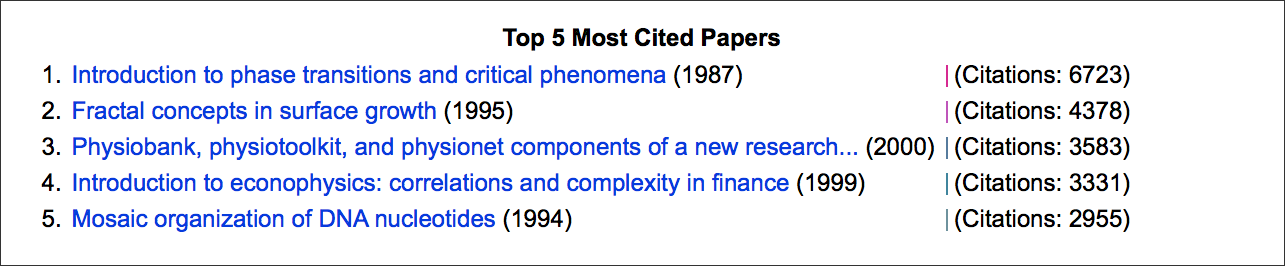
\includegraphics[width=\textwidth]{figures/fig_panel3-N}
    \caption{Panel highlighting the top 5 cited papers of the selected scholar.}
    \label{fig:panel3}
\end{figure}

\begin{figure}[H]
    \centering
    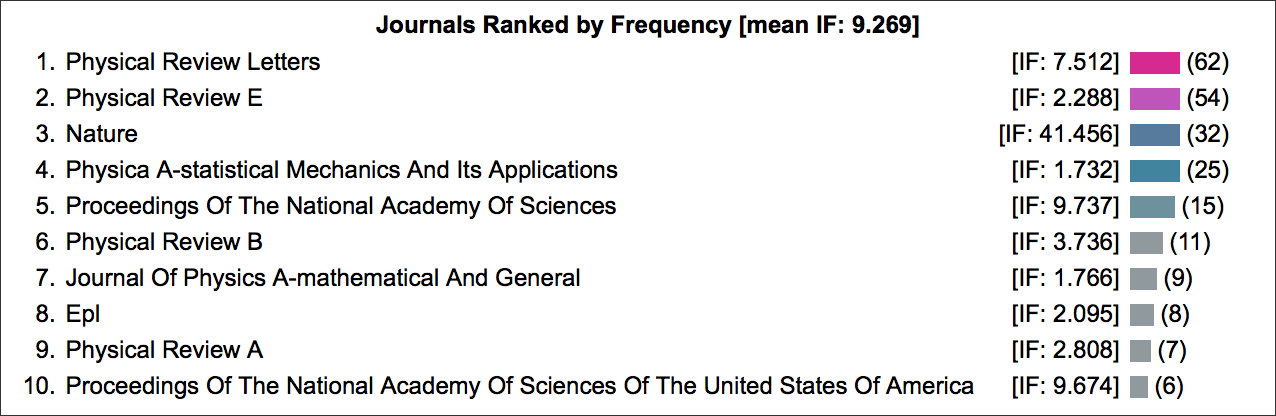
\includegraphics[width=\textwidth]{figures/fig_panel2-N}
    \caption{Panel displaying the top journals ranked by the frequency of publication.}
    \label{fig:panel2}
\end{figure}

\begin{figure}[H]
    \centering
    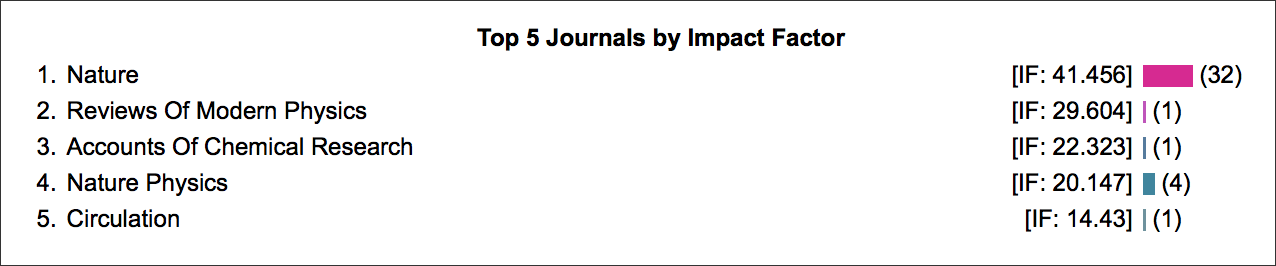
\includegraphics[width=\textwidth]{figures/fig_panel4-N}
    \caption{Panel showing the top 5 journals where the selected scholar published ranked by the impact factor.}
    \label{fig:panel4}
\end{figure}




% --------------------------
\section{Global and Local Bias Correction}
% --------------------------
%Academic Garden reveals that people look relatively important locally in low ranking departments, like University of Houston, (See Figure: \ref{fig:uh-local}) but there are not so important in the global scheme of visualization (See Figure: \ref{fig:uh-global}). The opposite is true for very high ranking departments, like MIT, where many people might look unimportant locally (See Figure: \ref{fig:mit-local}) because of a couple of outstanding people within the department even though they are quite good in their discipline (See Figure: \ref{fig:mit-global}).

Academic Garden reveals that some people stand out locally in low ranking departments such as the University of Houston (See Figure: \ref{fig:uh-local}) but are ordinary in the global scheme of visualization (See Figure: \ref{fig:uh-global}). The opposite is true for very high-ranking departments such as Massachusetts Institute of Technology (MIT) where, because of a couple of outstanding people, others may appear unimportant locally (See Figure: \ref{fig:mit-local}) though they are quite good in their discipline (See Figure: \ref{fig:uh-global}).

Providing both visualization schemes to the user makes Academic Garden a useful tool for every academic department no matter how they are ranked. 
Rather than a log scale, which would unjustifiably elevate the lowest performing faculty and not adequate acknowledge the merit of the highest performing faculty, the local scheme displays a department using a linear scale. The local scale is dynamic and is adjusted to the maximum citation count of the department.

The global scale has two linear sections. The top section has a fixed minimum of 20,001 and a fixed maximum of 300,000, which is larger than the highest number of citations in the global dataset. The bottom section has a fixed range of 0-20,000 citations, which represents the $90^{\text{th}}$ percentile of the global dataset. The larger height of the bottom section displays the $90^{\text{th}}$ percentile of faculty vertically across Academic Garden instead of compressing it to the very bottom.

\begin{figure}[H]
    \centering
    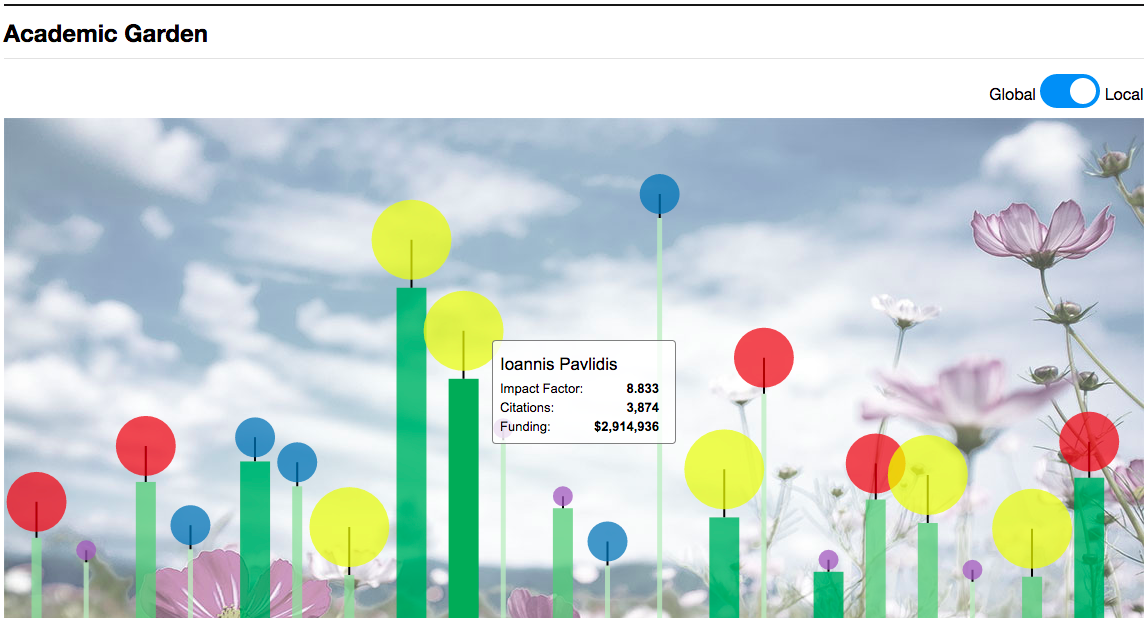
\includegraphics[width=0.9\textwidth]{figures/fig-UH-Local}
    \caption{Local Scale: Department of Computer Science at the University of Houston.}
    \label{fig:uh-local}
\end{figure}

\begin{figure}[H]
    \centering
    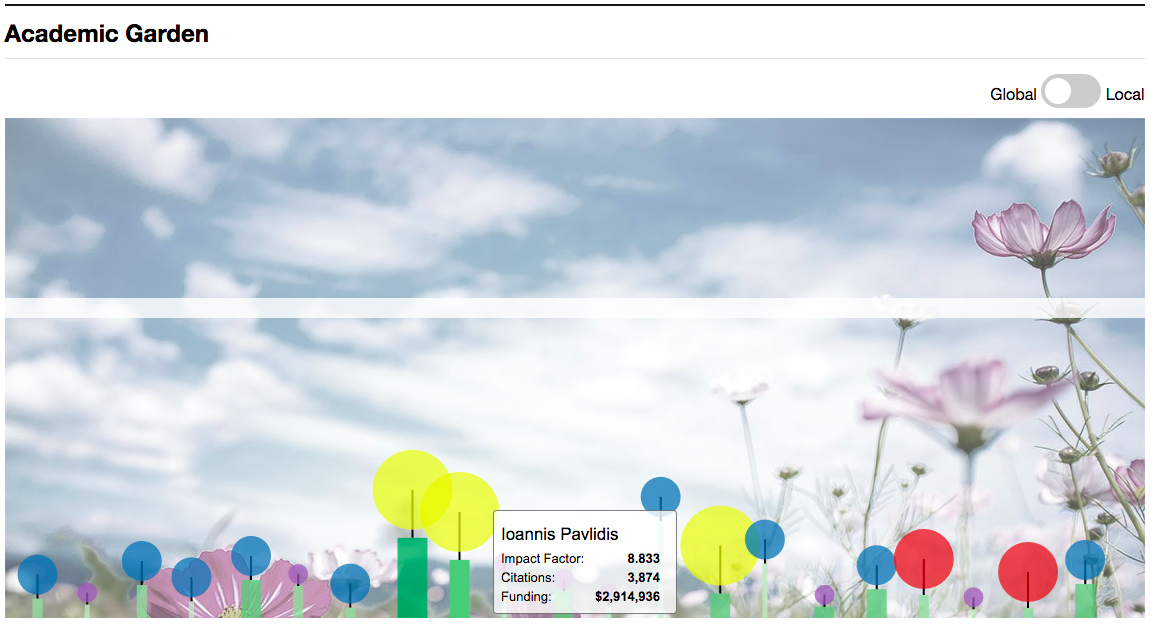
\includegraphics[width=0.9\textwidth]{figures/fig-UH-Global}
    \caption{Global Scale: Department of Computer Science at the University of Houston.}
    \label{fig:uh-global}
\end{figure}



\begin{figure}[H]
    \centering
    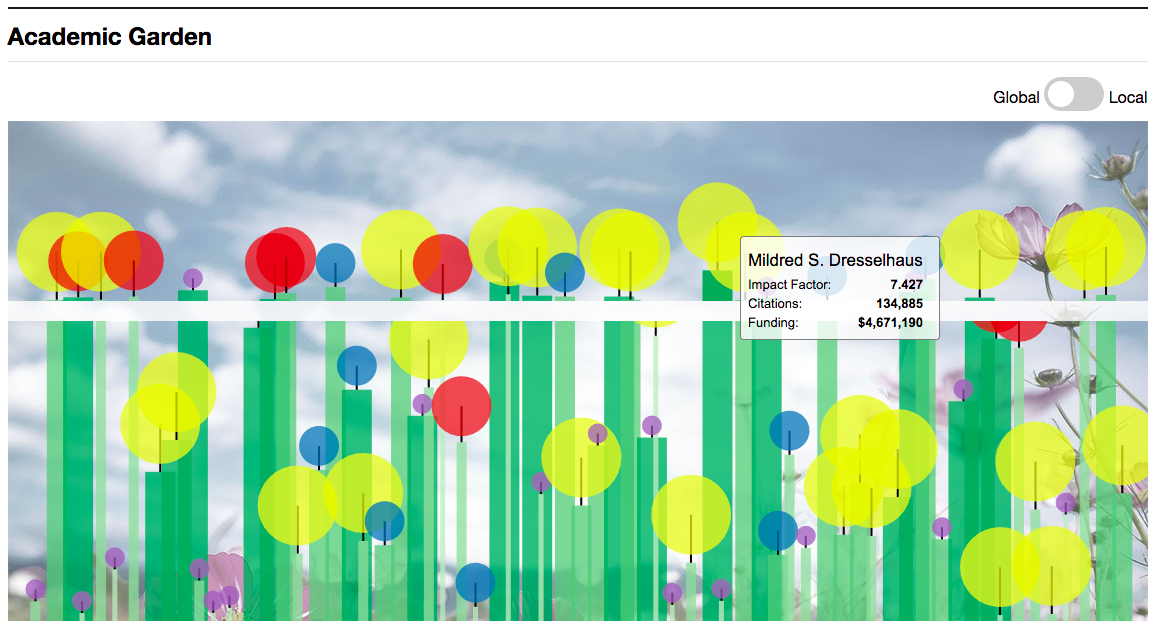
\includegraphics[width=0.9\textwidth]{figures/fig-MIT-Global}
    \caption{Global Scale: Department of Computer Science at the MIT.}
    \label{fig:mit-global}
\end{figure}

\begin{figure}[H]
    \centering
    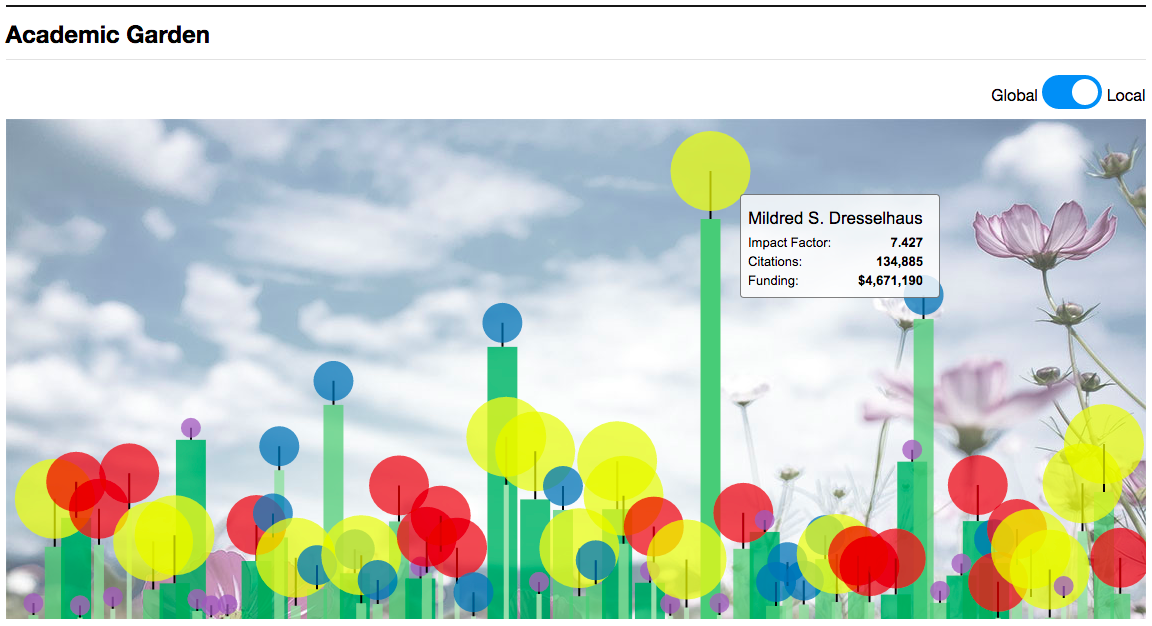
\includegraphics[width=0.9\textwidth]{figures/fig-MIT-Local}
    \caption{Local Scale: Department of Computer Science at the MIT.}
    \label{fig:mit-local}
\end{figure}





% --------------------------
\section{Data Analysis}
% --------------------------
For the validation of our design choices of Academic Garden, I used chaired faculty as the ground truth. An Endowed Chair is considered a prestigious award in the United States. I ran linear models in R software \cite{R:The81:online} to understand the validity of the design with respect to Endowed Chairs. 

The data was collected in July 2016. This included total 14 different universities. The data consists of $( n = 248 )$ faculty from Computer Science and $( n = 152 )$ from Biology from the top 10 schools according the US News Report 2015 \cite{usnews}. The data of chaired faculty consists of $( n = 61 )$ chaired professors from Computer Science and  $( n = 32 )$ from Biology in top 10 schools.


% For tables use
\begin{table*}
\centering
% table caption is above the table
\caption{The list of institutes in Computer Science by rank sourced from U.S. News \cite{usnews}.}
\label{tab:1}       % Give a unique label
% For LaTeX tables use
\begin{tabular}{rl}
\hline\noalign{\smallskip}
Rank & Department of Computer Science \\
\noalign{\smallskip}\hline\noalign{\smallskip}
1 & University of California, Berkeley \\
1 & Carnegie Mellon University \\
1 & Massachusetts Institute of Technology \\
1 & Stanford University \\
5 & University of Illinois at Urbana-Champaign \\
6 & Cornell University \\
6 & University of Washington \\
8 & Princeton University \\
9 & Georgia Institute of Technology \\
10 & University of Texas, Austin  \\
\noalign{\smallskip}\hline
\end{tabular}
\end{table*}



% For tables use
\begin{table*}
\centering
% table caption is above the table
\caption{The list of institutes in Biology by rank sourced from U.S. News \cite{usnews}.}
\label{tab:}       % Give a unique label
% For LaTeX tables use
\begin{tabular}{rl}
\hline\noalign{\smallskip}
Rank & Department of Biology  \\
\noalign{\smallskip}\hline\noalign{\smallskip}
1 & Harvard University \\
1 & Massachusetts Institute of Technology \\
1 & Stanford University \\
4 & University of California, Berkeley \\
5 & California Institute of Technology \\
5 & Johns Hopkins University \\
7 & University of California San Francisco \\
7 & Yale University \\
9 & Princeton University \\
10 & Cornell University \\

\noalign{\smallskip}\hline
\end{tabular}
\end{table*}

The three criteria we used in the Academic Garden are citations, impact factor, and funding. We computed the quartiles for these three criteria based on the local department faculty, as well as the global scale considering all the faculty from the same discipline. We obtained the discipline information from the Classification of Instructional Programs (CIP) codes from The National Center for Education Statistics designed the Classification of Instructional Program \cite{CIPus76:online}.


For each faculty, we computed the quartile to which he belongs to for each of the three criteria in the local and global scales. We also computed a variable to determine if a faculty belongs to either one of the top 3 criteria.
For Computer Science, this variable significantly predicts chaired faculty ( p $<$ 0.05 ) i.e, we can predict a faculty is chaired if he belongs to the top quartile locally in either of the three criteria.

The values are seen in Figures \ref{fig:CS-Local-Quartile}. In this model, quartiles are calculated with respect to the department which the faculty belongs to.

 \begin{figure}
  \centering
  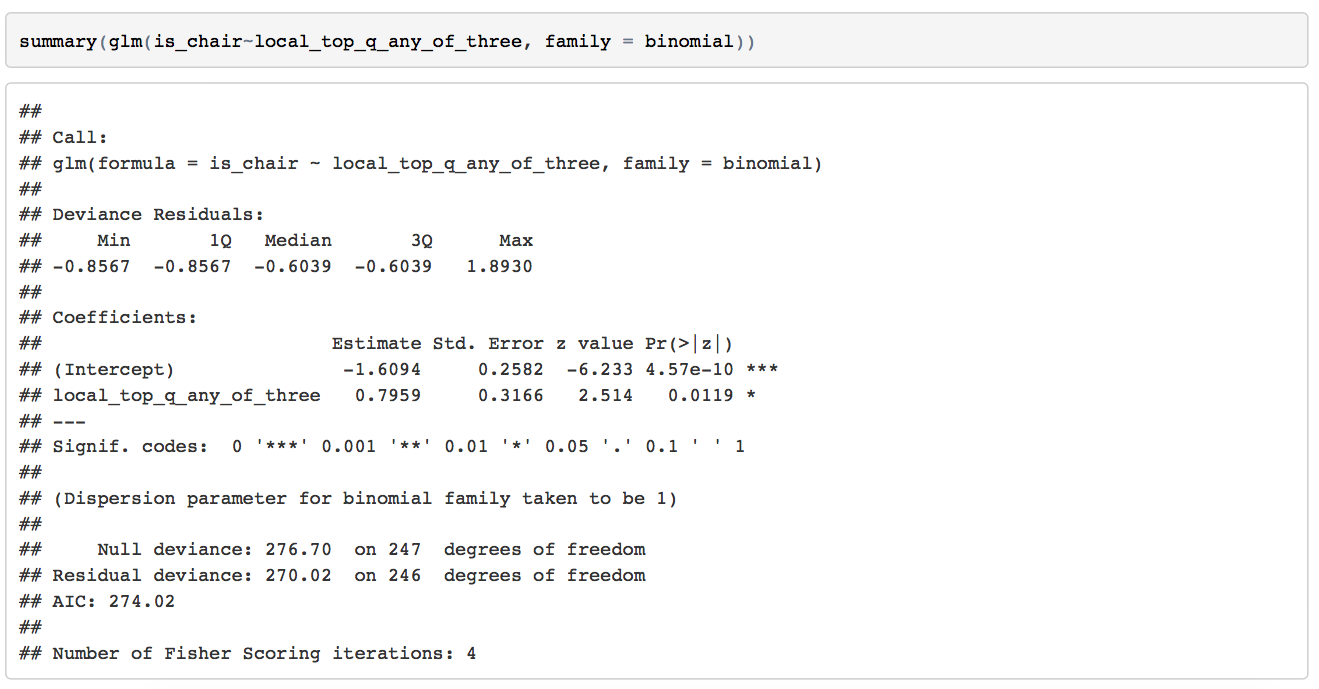
\includegraphics[width=\textwidth]{figures/CS-Local-Quartile}
%  \vspace{-3ex}
  \caption{Screenshot of a result of Linear Model in R.}
  \label{fig:CS-Local-Quartile}
\end{figure}

All three criteria can be considered as separate factors. In computer science, citations are highly significant ( p $<$ 0.001 ) while the mean impact factor is not significant. This is because computer science faculty do not publish as much in journals. The funding is also not significant because our funding sources (NSF/NIH/NASA) do not include most funding sources which computer science faculty obtains funding, for example, DoD (United States Department of Defense) and DHS (United States Department of Homeland Security).

However, in the case of Biology, the funding quartile is significant ( p $<$ 0.01 ) because of the funding dataset includes NSF, NIH from where most the Biology grants are from (Figures: \ref{fig:BIO-local-funding}). Also, the Impact Factor quartile is significant ( p $<$ 0.05 ) because they publish more in journals.

 \begin{figure}
  \centering
  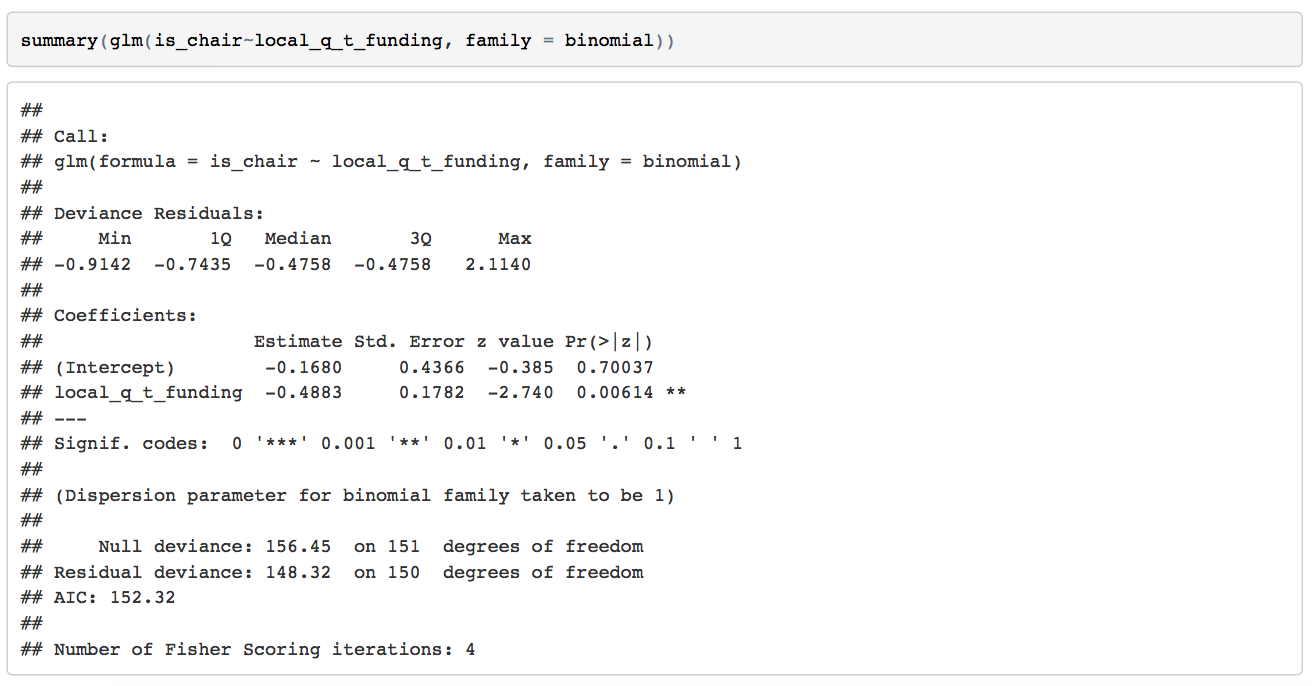
\includegraphics[width=\textwidth]{figures/BIO-local-funding}
%  \vspace{-3ex}
  \caption{Screenshot of a result of Linear Model in R.}
  \label{fig:BIO-local-funding}
\end{figure}

According to the results of linear model, the data analysis validates the design choice of the three criteria for the visualization, and it is exactly mirroring visualization with quartiles values.




%1.	Biologists publish less than computer scientists and have more authors per paper. The mean number of publications per year in Biology (5.21) is significantly lower (t-test, p < 0.01) than the respective mean in Computer Science (8.58). In contrast, the mean number of coauthors in Biology publications (5.57) is significantly higher (t-test, p < 0.01) than the respective mean in Computer Science (4.71).

%2.	Biologists publish mainly in journals, while Computer Scientists less so. The percentage of journal publications is significantly higher (t-test, p < 0.01) in Biology (73.36\%) with respect to Computer Science (19.83\%).

%3.	Biology's elite dominates publications in their top journals a lot more than the Computer Science elite does in theirs. Within the ranked set of all Biology journals, our Biology faculty sample publishes in the top 11\%. In contrast, within the ranked set of all Computer Science journals, our Computer Science faculty sample publishes in the top 24\%. 

%4.	There is significant correlation between the citations obtained per year versus the number of publications produced per year in both disciplines, with Biology (p < 0.01,  = 81.15, R2 = 0.54) having a steeper slope than Computer Science (p = 0.01,  = 40.81, R2 = 0.19). The latter suggests that Biology has a tendency for higher mean citation-impact per article than Computer Science.



\chapter{Conclusion}\label{chap:Conclusion}

We have described a visualization method that complements the information contained in a researcher's Google Scholar page and summarized by her/his {\it h}-index. One can draw insightful conclusions about the individual's scholastic accomplishments. These conclusions are not supported by the {\it h}-index alone and cannot be derived by the CV or the Google Scholar page, unless a significant investigative effort is undertaken. Our user study also supports this.

This approach not only focusses on journal publications, conferences / books and patents but also NSF/NIH funding data. Scholar Plot is a simple, yet valuable visualization scheme. It is likely to have broad appeal not only because it would be useful to evaluation committees, but also because it is available online for free at \url{http://www.scholarplot.com}. 

%\section{Summary of Contributions}
%
%\subsection{Image Segmentation}
%
%\subsection{Cardiac Morphology and Function}
%
%\subsection{Coronary Artery Shape-Motion Analysis}
%
%%%%%%%%%%%%%%%%%%%%%%%%%%%%%%%%%%%%%%%%%%%%%%%%%%%%%%%%%%%%%%%%
%\section{Progression and Scope for Future Work}
%
%
%\subsection{Algorithm for the Automatic LV Blood Pool Segmentation
%from Short-Axis Dual-Contrast MR Data}
%
%%%%%%%%%%%%%%%%%%%%%%%%%%%%%%%%%%%%%%%%%%%%%%%%%%%%%%%%%%%%%%%%
%\subsection{Algorithm for the Automatic Delineation of Myocardial
%Contours in Short-Axis Cardiac Cine-bFFE MR Sequences}
%
%
%%%%%%%%%%%%%%%%%%%%%%%%%%%%%%%%%%%%%%%%%%%%%%%%%%%%%%%%%%%%%%%%
%\subsection{Algorithm for the Automatic Computation of EF from the Short-Axis Cardiac Cine-bFFE MR Sequences}
%
%
%%%%%%%%%%%%%%%%%%%%%%%%%%%%%%%%%%%%%%%%%%%%%%%%%%%%%%%%%%%%%%%%
%\subsection{Computational Framework for the 4D
%Shape-Motion Analysis of the LAD}
%
%
%%%%%%%%%%%%%%%%%%%%%%%%%%%%%%%%%%%%%%%%%%%%%%%%%%%%%%%%%%%%%%%%
%\subsection{Future Work}
%
%%%%%%%%%%%%%%%%%%%%%%%%%%%%%%%%%%%%%%%%%%%%%%%%%%%%%%%%%%%%%%%%

%% ==================================================
  \chapter{Introduction}\label{chap:Intro}
% ==================================================
A curriculum vitae (CV) provides a synopsis of an individual's achievements. The CV content varies by profession. Academic CVs feature prominently a publication section. This section references the researcher's journal papers and other scholarly products.

Search, promotion, and award committees that screen CVs go through lists of publications trying to form opinions about the candidates' records. Does candidate A or B have enough publications? Are they of high quality? Did they have any impact on the research community?
In a highly competitive context, these questions do not always have clear answers. Another question that needs to be addressed is whether the candidate has been funded. If so, has the candidate done justice to the amount of funds obtained? This also enables one to decide if the candidate's output is in proportion with the input.














% ==================================================
\chapter{Background}\label{chap:Background}
% ==================================================

There has been some work on the quantification of academic careers, focused on a quest for a `number' that sums up an academic's scholarship. The most well-known outcome of this line of research is the {\it h}-index, proposed by Hirsch \cite{Hirsch:2005}. A scholar has an index of {\it h} if s/he has published {\it h} papers each of which has been cited in other papers at least {\it h} times (Figure \ref{fig-hindex}).

\begin{figure*}
    \centering
    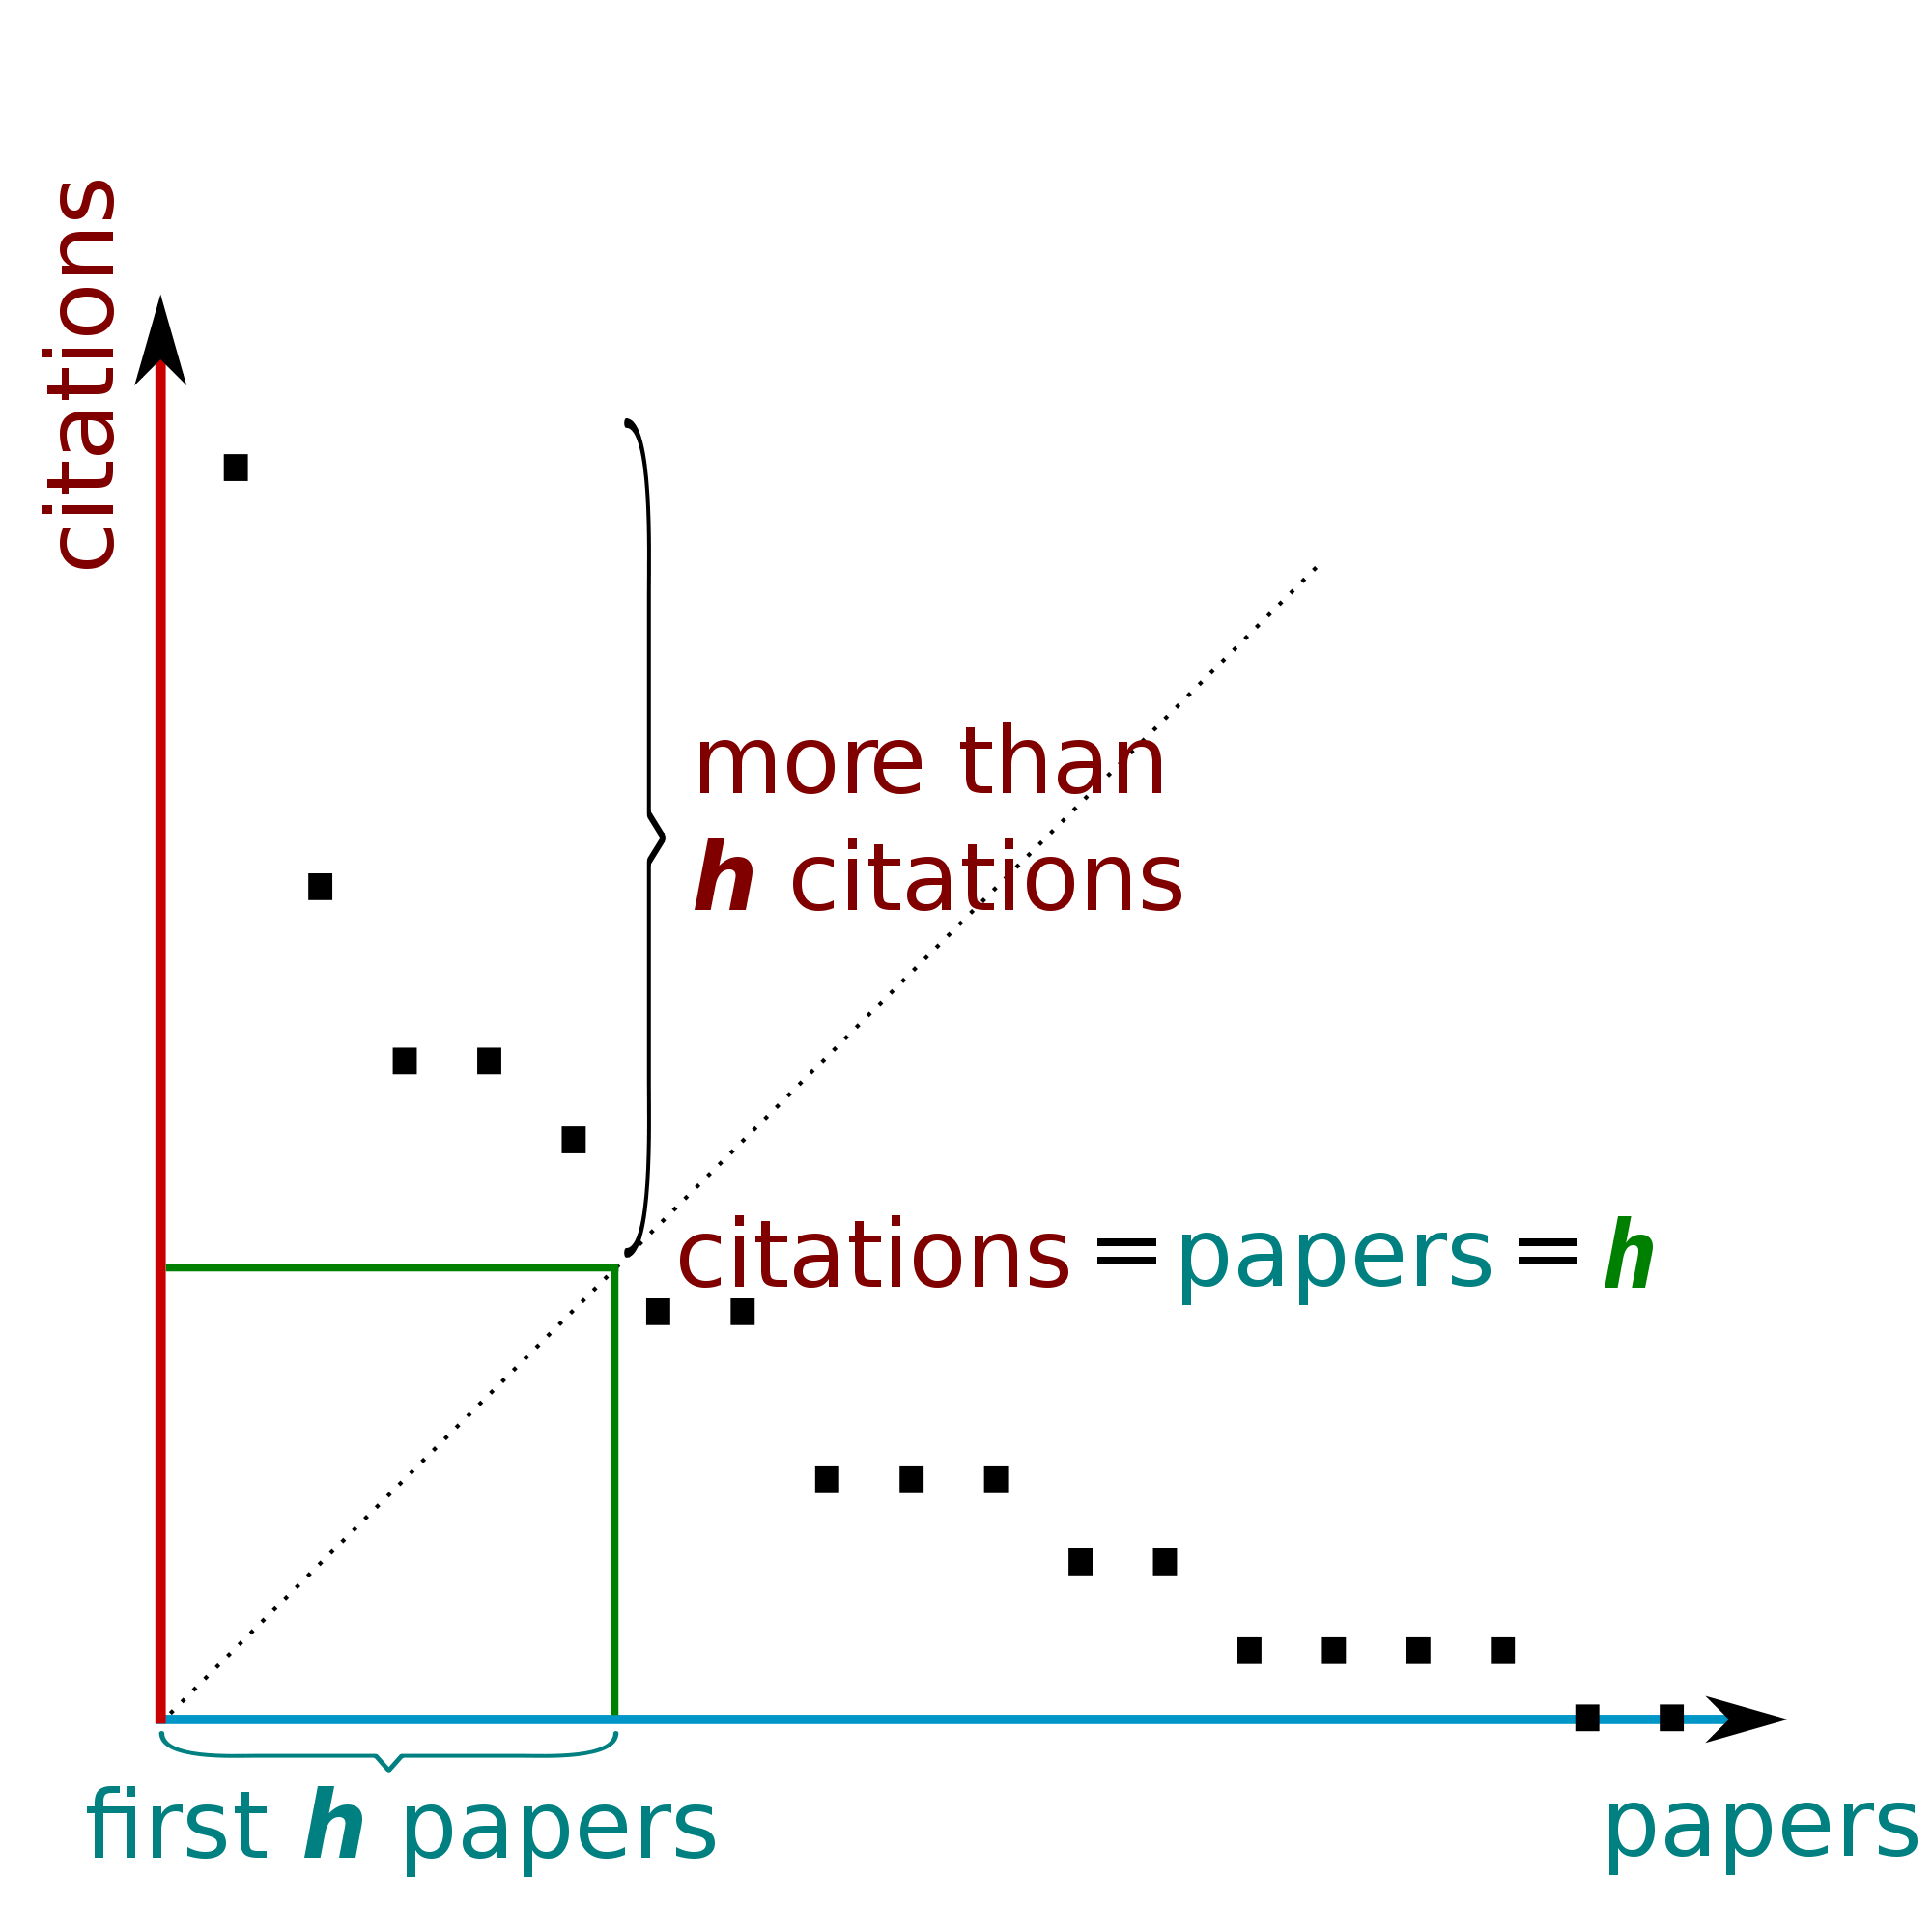
\includegraphics[width=1\textwidth]{figures/H-index.png}
    \caption{h-index from a plot of decreasing citations for numbered papers}~\label{fig-hindex}
\end{figure*}


The {\it h}-index depends on both the number of publications and the number of citations. Hirsch demonstrated that {\it h} can predict honors, such as National Academy membership and Nobel prize. He also suggested that it could predict advancement to tenure, although with some uncertainty.
Despite its value, the {\it h}-index has weaknesses and when used, context should be carefully taken into account; such context includes the academic field and the academic age of the candidate \cite{Bornmann2}.

With the advent of Google Scholar, information about a researcher's publication record and her/his {\it h}-index has become easily accessible. Then, with the ease of access of the internet, this information has become ubiquitous.

In this dissertation I introduce data visualization methods that complement the publication information contained in a standard CV and summarized by the {\it h}-index. The tool produces a temporal visualization that connects the {\it h}-index with the paper citations and the journal impact factors along with the funding data.

There have been other efforts in visualizing patterns of scientific production and impact \cite{Katy:2010, Chen:2001, Leydesdorff:2007}. Recently, a mobile app (DBIScholar) has also appeared that interfaces information from Google Scholar \cite{sabrina741}. A social tool named Scholarometer has been developed to facilitate citation analysis and to evaluate the impact of authors \cite{Kaur:2014}. This tool helps to visualize author and discipline networks. There is another tool called SciVal Expert to visualize the collaboration and research output of institutions \cite{Vardell:2011}. This tool uses data from Scopus. But these tools do not provide a visual picture of a single scholar's achievements.

Our method and application differ from the prior art. Scholar Plot helps the reviewer determine at a glance from where the researcher's impact (if any) arises from.% : citations in articles published in low impact journals or citations in articles published in high impact journals.

Even students need more information to decide about their college. Nowadays, a university has a ranking as well as each department with each college in that university. So students need publicly accessible information which is cheap and get a summary of various measures being used to evaluate faculty. Rankings are used to make choices to avoid risks of joining lower ranking colleges \cite{mcdonough1998college}.

With the advent of Google Scholar, information about a researcher's publication record and her/his {\it h}-index has become easily accessible. Then, with the ease of access of the internet, this information has become ubiquitous.

Our goal is to articulate a clear, comprehensive, and measurable performance evaluation scheme for academics. This scheme should reveal causal relationships among the merit criteria. We provide a summary interface to facilitate executive decisions. The tool produces a temporal visualization that connects the {\it h}-index with the paper citations and the journal impact factors along with the funding data. Scholar Plot helps the reviewer determine at a glance from where the researcher's impact (if any) arises from.

In this article we introduce a data visualization tool that complements the publication information contained in a standard CV and summarized by the {\it h}-index.

We introduce a data visualization tool that complements the US News Rankings and the publication information contained in a standard CV. Visualization facilitates access to data and supports actionable insights \cite{Yi:2008:UCI}. It also helps to bring out patterns and pattern violations in the underlying data.
The tool produces a temporal visualization that connects the {\it h}-index with the paper citations and the impact factors along with the funding data. Our method and application differ from the prior art. Scholar Plot helps the reviewer determine at a glance from where the researcher's impact (if any) arises from. It also gives a hierarchical view of accomplishments from a single author to the department to the entire college.






% ==================================================
\chapter{Methods}\label{chap:Methods }
% ==================================================

In this section, I will explain various criteria for evaluating academic performance, individual visualization (Scholar Plot) and group visualization (Department Plot) and Academic Garden which is a scalable visualization of academic merit.


% --------------------------
\section{Design Process}
% --------------------------
There are various criteria for evaluating academic performance. We focus on three main criteria.
\begin{itemize}
\item \textbf{Impact} - it is the post-production merit. For example, the citations which a publication receives. A publication with higher number of citations has higher visibility. Therefore, we linked the impact to the vertical axis in the plot.
\item \textbf{Prestige} - this is the pre-production merit associated with the venue of publication. For example, the impact factor of a journal is the merit your publication will acquire because it has been published in that journal. Hence we associate a disk with variable sizes to the prestige of the venue. We consider it as a `fancy factor`.
\item \textbf{Funding} - it enables the production of publications/research. Hence we place it at the bottom of the plot. This can help to correlate the production with the funding.
\end{itemize}

ScholarPlot uses publicly available publication and affiliation information on researchers, scholars, and authors for the purpose of visualizing popular indicators of publishing activity. No single set of indicators can capture all the dimensions of a publication's scholarly value or an author's contributions to knowledge. Depending on a user's objective, ScholarPlot maybe best used in combination with other measures. Our visualization consists of a hierarchy of visualization schemes right from the individual to the department and the college.









% =============================================================================
\section{Scholar Plot - Individual Visualization}
% =============================================================================
Scholar Plot obtains the Impact Factor ($IF$) for a particular journal from our database. The data of Impact Factor is acquired from The Thomson Reuters Impact Factor - Web of Science. Based on all this information it constructs the plots as per the design outlined in the Visualization and User Interface section, using nvd3 library \cite{nvd3org}.


The NSF/NIH/NASA funding datasets are available at the respective US government websites in various file formats such as XML, CSV and so on \cite{nsf, nih}. We implemented a script to parse this massive XML dataset into our data structure that consists of AwardID, AwardAmount, First name, Last name, Investigator by RoleCode (Principal Investigator, Co-Principal Investigator and Former Principal Investigator), using XMLStarlet \cite{XMLStarlet}. We imported this data to our database using Toad DBMS tool. %We designed our relational database schema in MySQL.

\begin{figure}%[!htb]
\centering
  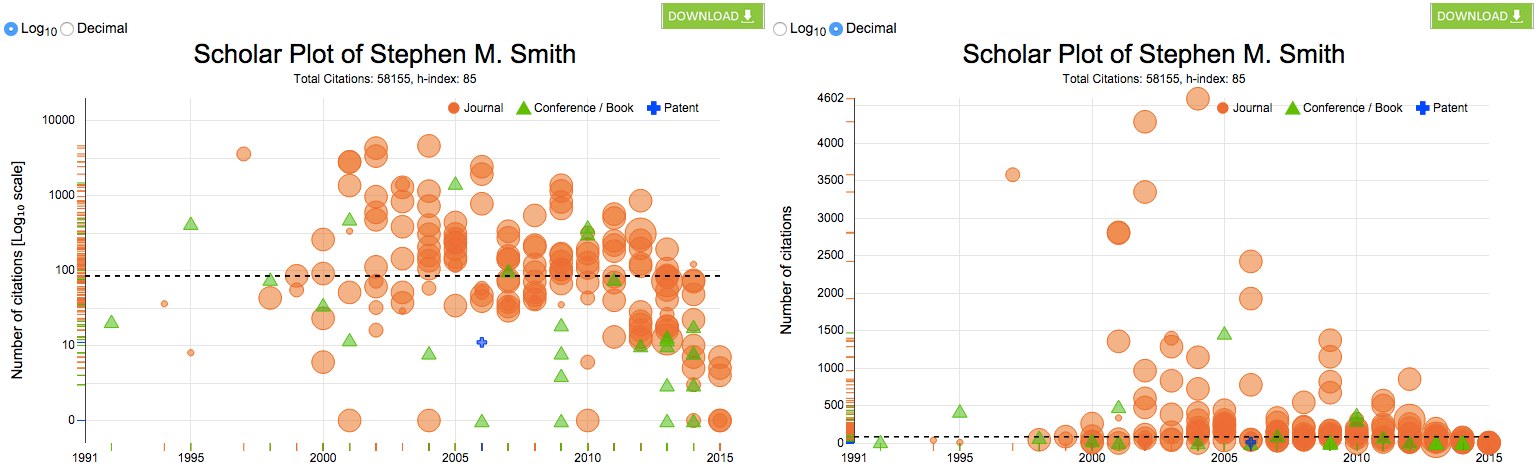
\includegraphics[width=1\textwidth]{figures/fig_scaleView}
  \caption{The $log_{10}$ view and $decimal$ view: The radio button allows to switch between different scale views without reloading the entire page.}~\label{fig-scale}
\end{figure}

\begin{figure*}
  \centering
  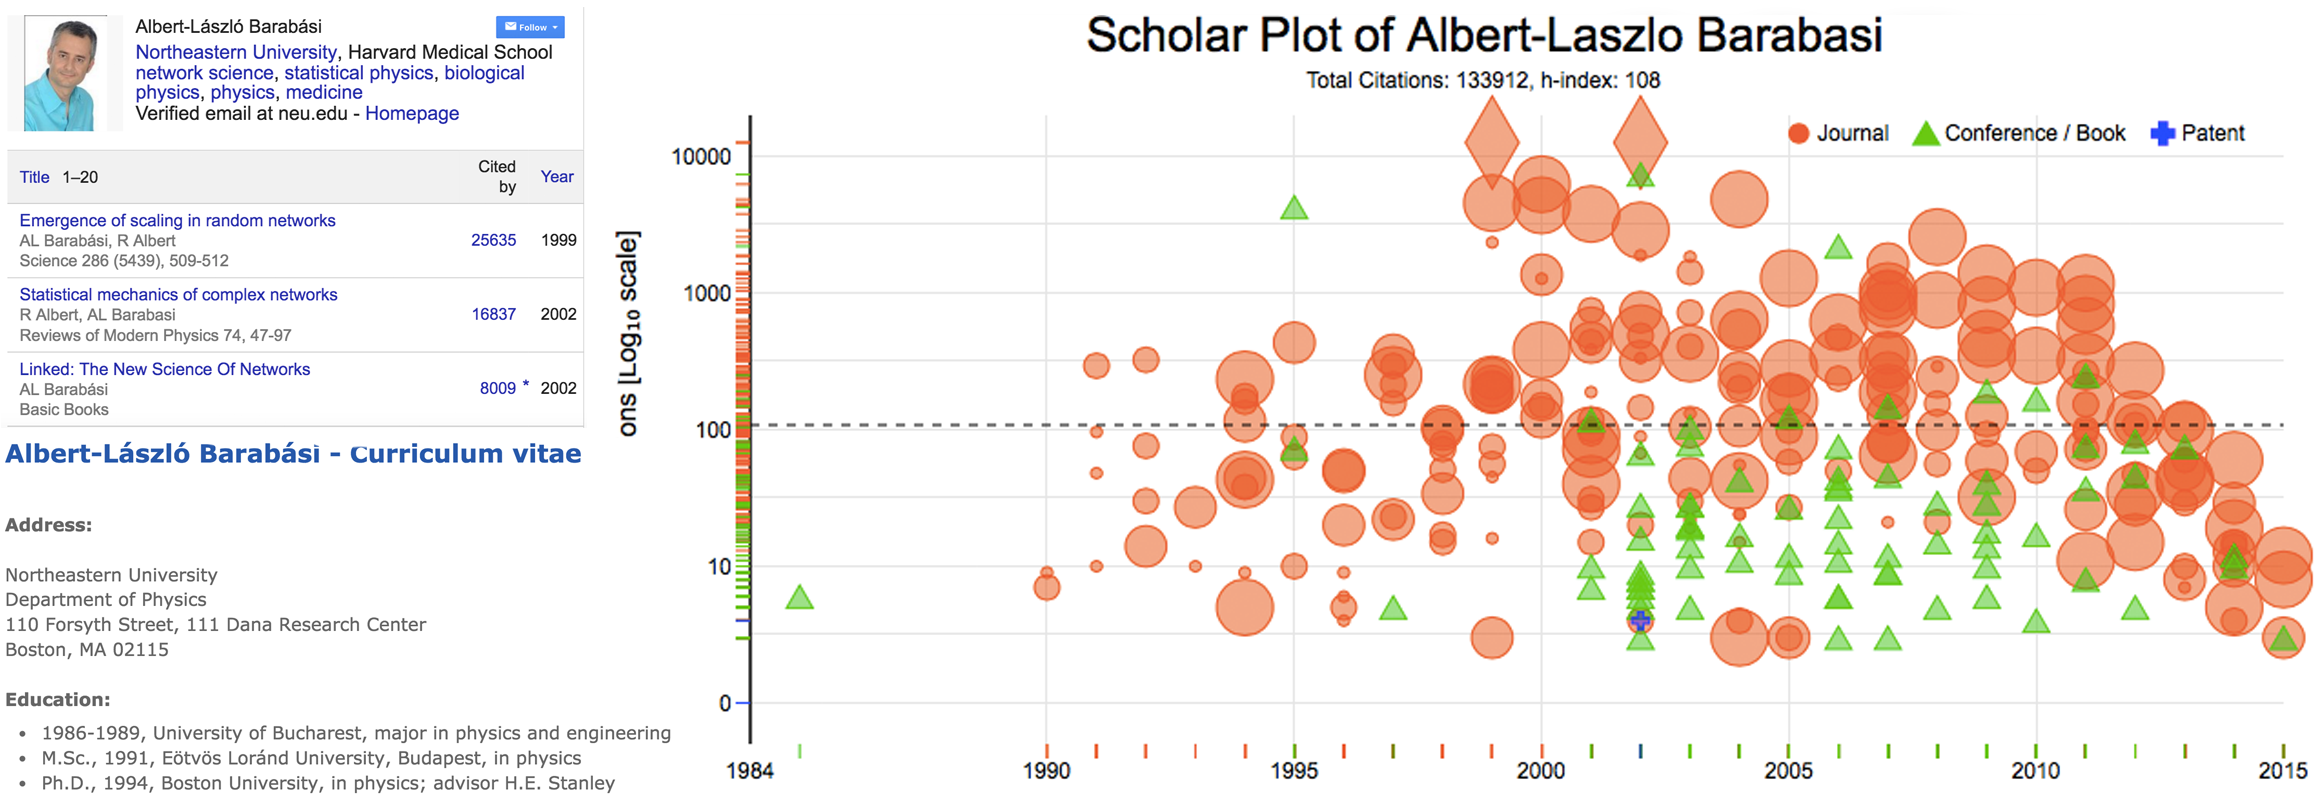
\includegraphics[width=1\textwidth]{figures/fig_publication}
  \caption{An example of Scholar Plot - Visualizing Publication Data}~\label{fig-publication}
 % \vspace{-1ex}
\end{figure*}

% \begin{figure*}
%   \centering
%   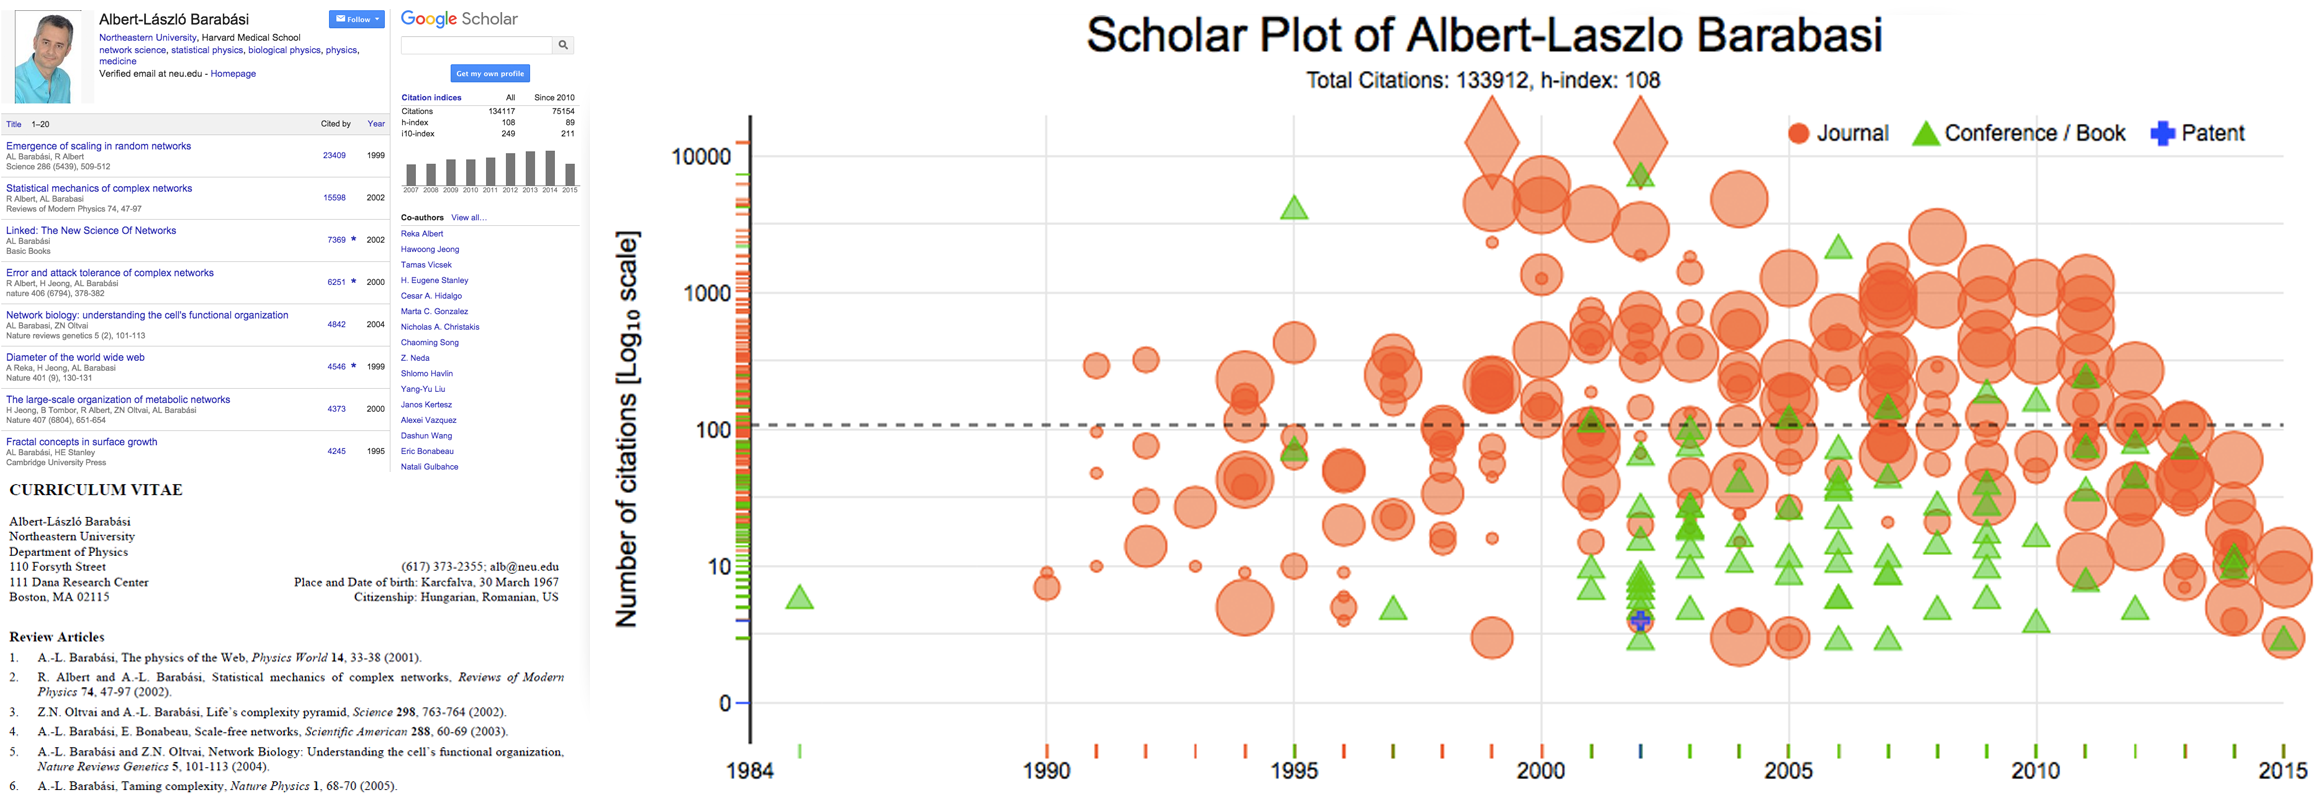
\includegraphics[width=1\textwidth]{figures/fig_cv_google_scholarplot}
%   \caption{An example of Scholar Plot - Visualizing Publication Data}~\label{fig-publication}
%  % \vspace{-1ex}
% \end{figure*}

Scholar Plot depicts the publications of an individual as a scatter plot and the NSF/NIH/NASA funding as a multiline plot. The publications are represented in a 2D diagram (number of citations vs. year of publication) with the {\it h}-index line (Figure \ref{fig-publication}). The horizontal axis is time, starting with the year of the researcher's first publication ending with the current year. The vertical axis is the number of citations. The default plot is in $log_{10}$ scale. The user can also view the plot in the decimal scale by a toggle option using a radio button at the top left corner (Figure \ref{fig-scale}). The log scale provides a standardized scale which helps to compare the plots of multiple scholars.



% --------------------------
\subsection{Publication Data}
% --------------------------
Each publication $i$ is represented with a symbol. The center of the symbol has coordinates $(i_{PY}, i_{C})$, where $PY$ stands for Publication Year and $C$ for Number of citations obtained by the publication till date. The journals are represented as circles (orange) with area analogous to the impact factor the journal. The conferences / books are represented as triangles (green) and the patents as crosses (blue). By clicking at a symbol you can obtain the publication title, the year, the number of citations, the venue where published and its impact factor (if it is a journal), as well as a breakdown in the authorship, complete with the level of collaboration between the co-authors and the selected scholar (Figure \ref{fig-tooltip}). The publication title also enables the user to navigate to the Google Scholar page for the selected paper. This helps to quickly verify and obtain further details of the selected publication. It makes user reach out to the PDF file directly if available. To enhance user experience, we customized the tooltip to give detailed information without overlapping the plots.

\begin{figure}[H]
\centering
  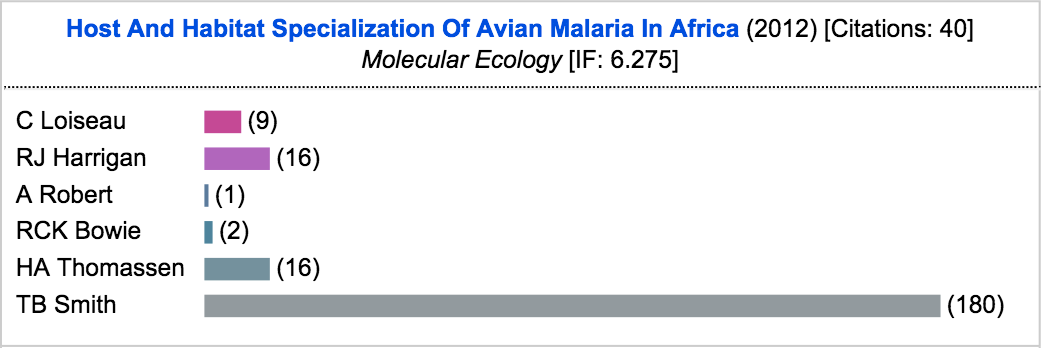
\includegraphics[width=1\textwidth]{figures/fig_tooltip}
  \caption{An example of the tooltip: The publication title, the year, the number of citations, the venue where published, impact factor, the list of co-authors, the visual horizontal bars with the number of collaboration between the co-authors and the selected scholar.}~\label{fig-tooltip}
 % \vspace{-1ex}
\end{figure}

A dotted horizontal line on the plot denote the {\it h}-index of the scholar. We also denote those publications which earn greater than 10,000 citations with diamonds as they represent the great success in publications (Figure \ref{fig-publication}). The title of the plot contains the name of the scholar and her/his total number of citations along with the {\it h}-index. At the top right corner of the plot, a legend shows the three different types of publications we distinctly display (Figure \ref{fig-legend}).

\begin{figure}[!htb]
\centering
  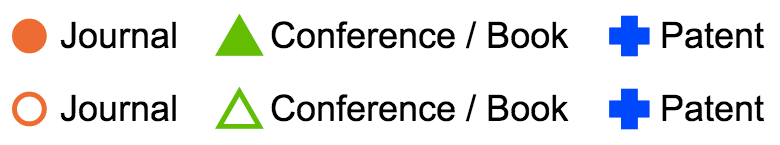
\includegraphics[width=1\textwidth]{figures/fig_legend-toggle}
  \caption{The legend allows users to selectively view journals, conferences / books and patents.}~\label{fig-legend}
 % \vspace{-1ex}
\end{figure}



\begin{figure*}
    \centering
    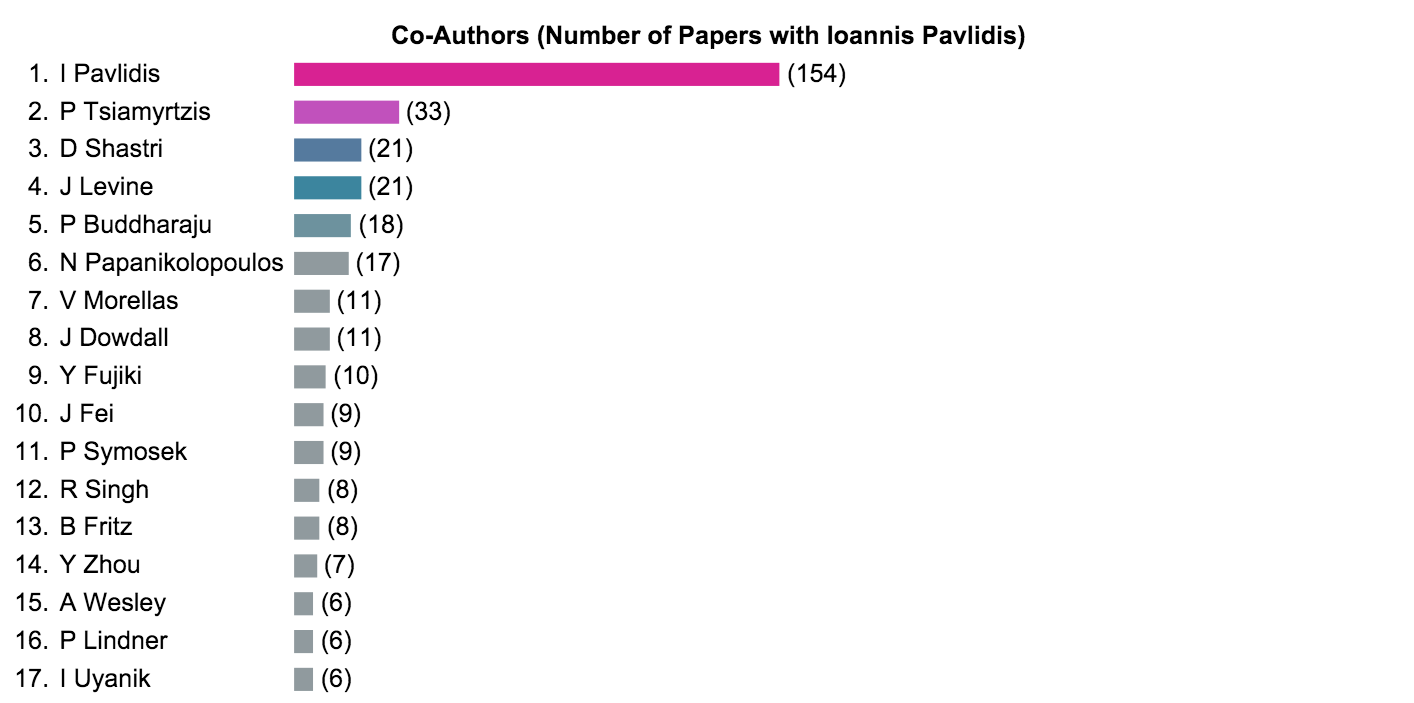
\includegraphics[width=1\textwidth]{figures/fig-panel-coauthros.png}
    \caption{The coauthor panel displays the author list.}~\label{fig-coauthors}
\end{figure*}




You can bring the journals, patents, and conferences / books in and out of the view by clicking at the respective legend. If there is an overlap between journals, conferences and patents, this feature can help the user to selectively view them. The user can also zoom into the plot for closer picture. Also note that the symbols are not completely opaque. So if there are multiple symbols which overlap, the user can see and interact with them by hovering the mouse over them appropriately.

% --------------------------
\subsection{Funding Data}
% --------------------------
Scholar Plot also depicts the NSF/NIH/NASA funding of an individual as a multiline (Figure \ref{fig:funding}). Each breakpoint in the multiline corresponds to the individual's total amount in all NSF/NIH/NASA awards for the specific year. By pointing at a breakpoint you can obtain the NSF/NIH/NASA awards IDs, award amounts, and investigator's role. The total annual funding information per year is also available by clicking the legend.

\begin{figure}[!htb]
  \centering
  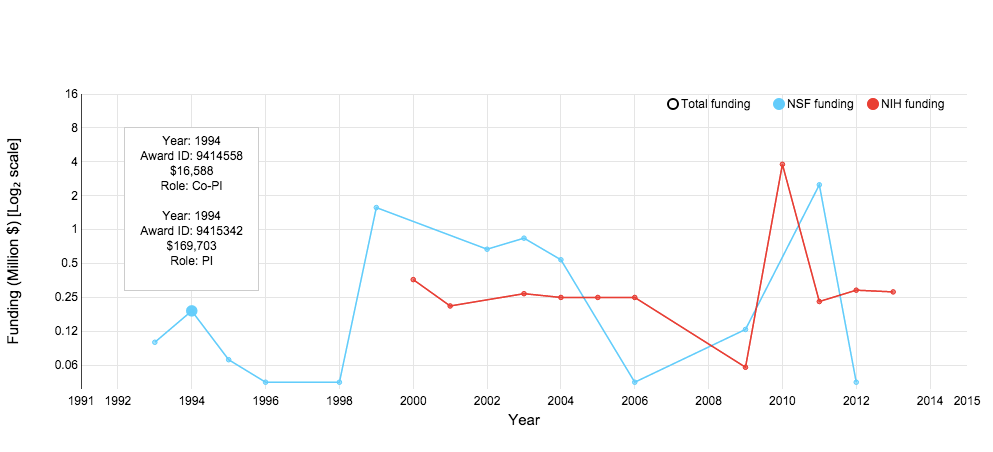
\includegraphics[width=1\textwidth]{figures/fig_funding_default}
  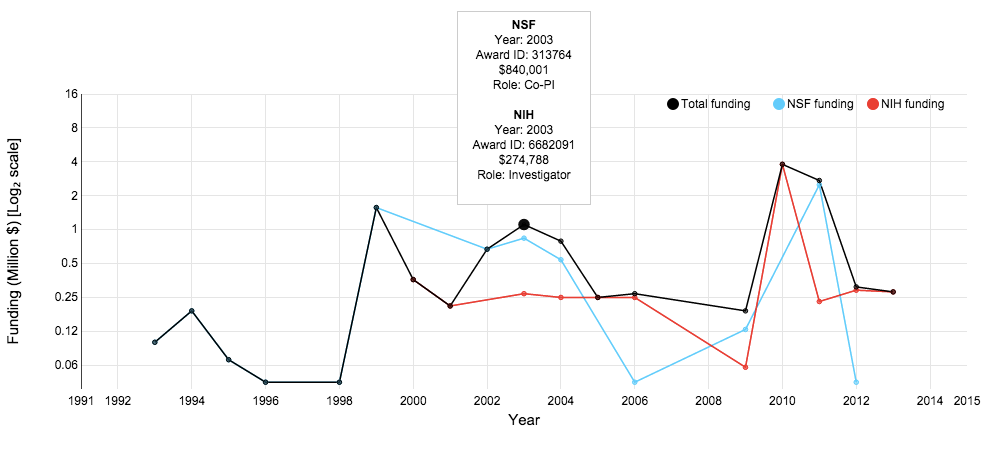
\includegraphics[width=1\textwidth]{figures/fig_funding_total}
  \caption{An example of Scholar Plot - Visualizing Funding Data}~\label{fig:funding}
  % \vspace{-2ex}
\end{figure}






% --------------------------
\section{Department Plot - Group Visualization}
% --------------------------
The group level of Scholar Plot visualizes department/college academic records. The issue we had to address was to determine how to scale the individual visualization to the group level. Group plot consists of 2 aspects - plot at the department level and at the college level. We apply our design philosophy at the group level. We use pie charts and bar charts (Figure \ref{fig:groupplot}) to display the information in a compact manner. Pie charts are also useful to show proportion of contribution of each individual to the group (i.e. department). For the pie-charts, we display the top 5 scholars to avoid over crowding the pie chart (Figure \ref{fig:Group-Cit}).

\begin{figure}[H]
  \centering
  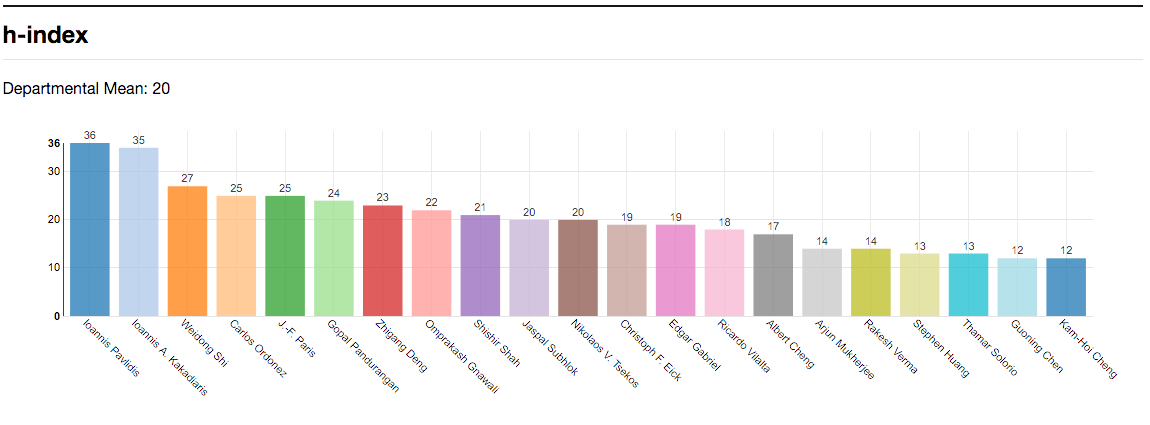
\includegraphics[width=1\textwidth]{figures/fig-CS-hIndex}
  \caption{Example of bar chart by h-index.}~\label{fig:groupplot}
\end{figure}

% --------------------------
\subsection{Department Plot}
% --------------------------

Departmental Plot is an attempt to visualize aspects of tenured and tenure-track faculty contributions to their home departments. These aspects are not only intellectual contributions and perhaps not even the most important. The faculty are compared based on publicly available measures like h-index, citations and impact factor. We show a citation contribution pie chart normalized by the number of years in which a scholar spent in academia. We also portray charts depicting the highest (Home Run) cited paper and the highest (Home Run) impact factor journal where the scholar published.

\begin{figure*}
  \centering
  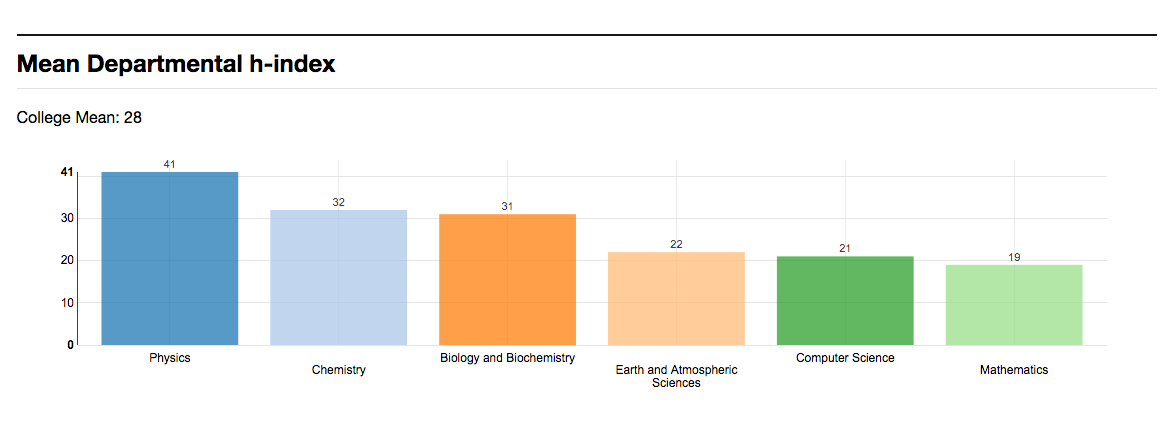
\includegraphics[width=1\textwidth]{figures/Coll-h}
  \caption{An example of departmnet plot - Colleg of Natural Science and Mathmatics at University of Houston - hIndex}~\label{fig:DP-College1}
\end{figure*}

\begin{figure*}
  \centering
  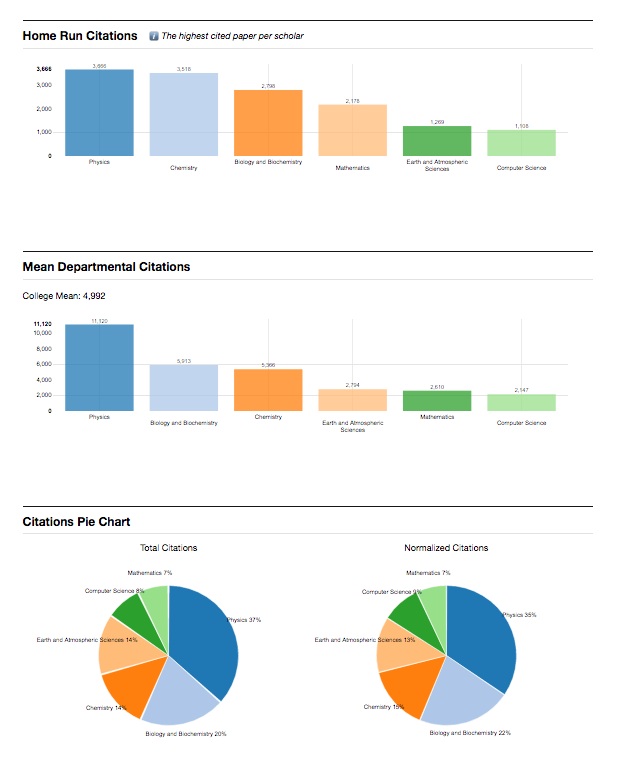
\includegraphics[width=1\textwidth]{figures/Coll-Cit}
  \caption{An example of departmnet plot - Colleg of Natural Science and Mathmatics at University of Houston - Citation}~\label{fig:DP-College1}
\end{figure*}

\begin{figure*}
  \centering
  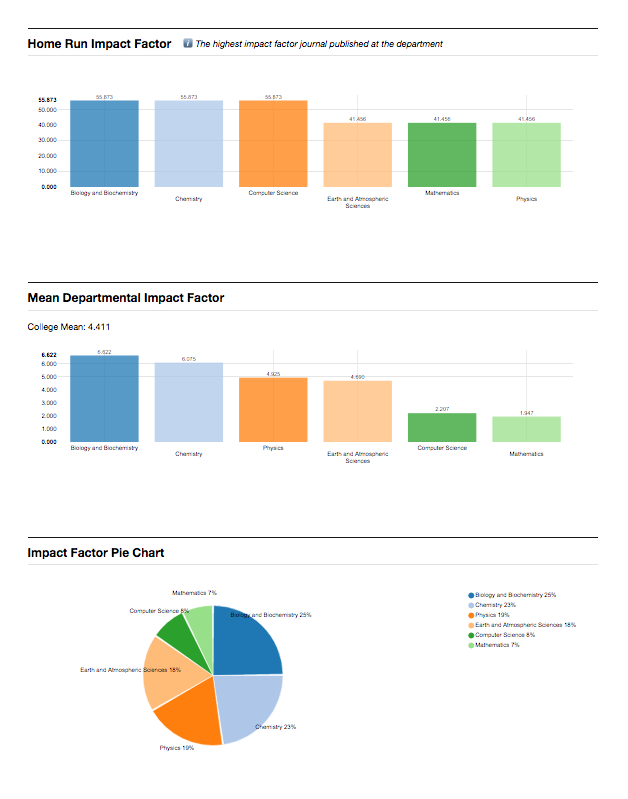
\includegraphics[width=1\textwidth]{figures/Coll-IF}
  \caption{An example of departmnet plot - Colleg of Natural Science and Mathmatics at University of Houston - Impact Factor}~\label{fig:DP-College1}
\end{figure*}

\begin{figure*}
  \centering
  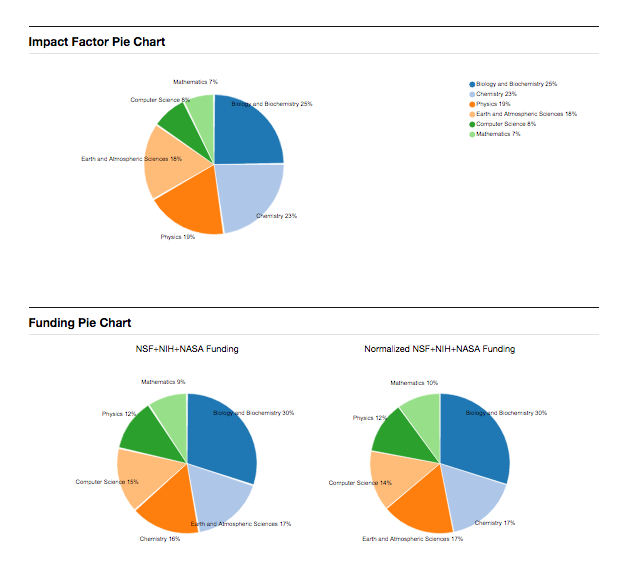
\includegraphics[width=1\textwidth]{figures/Coll-Fund}
  \caption{An example of departmnet plot - Colleg of Natural Science and Mathmatics at University of Houston - Funding}~\label{fig:DP-College1}
\end{figure*}



% --------------------------
\subsection{College Plot}
% --------------------------

College plot attempts to visualize the contributions of the departments to the home college. College plot pictures the mean values of various measures described above for each department. We use pie charts (Figure \ref{fig:Group-Cit}) and bar charts like in the department plot. Note that the data for department and college plot is generated using a query to our database. We are working on adding more universities to this database.


\begin{figure*}
  \centering
  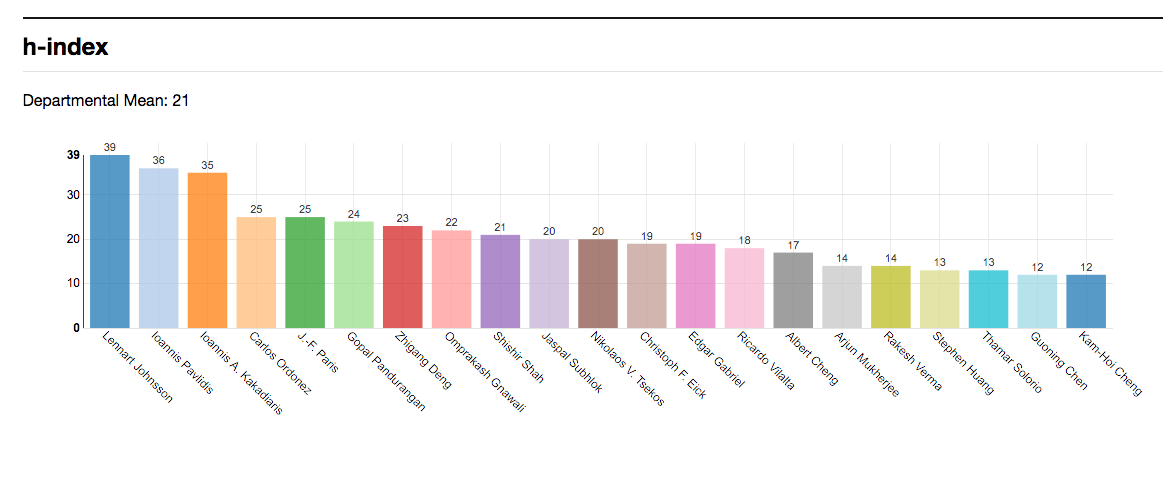
\includegraphics[width=1\textwidth]{figures/Dept-h}
  \caption{An example of departmnet plot - Department of Computer Science at University of Houston - hIndex}~\label{fig:DP-College1}
\end{figure*}

\begin{figure*}
  \centering
  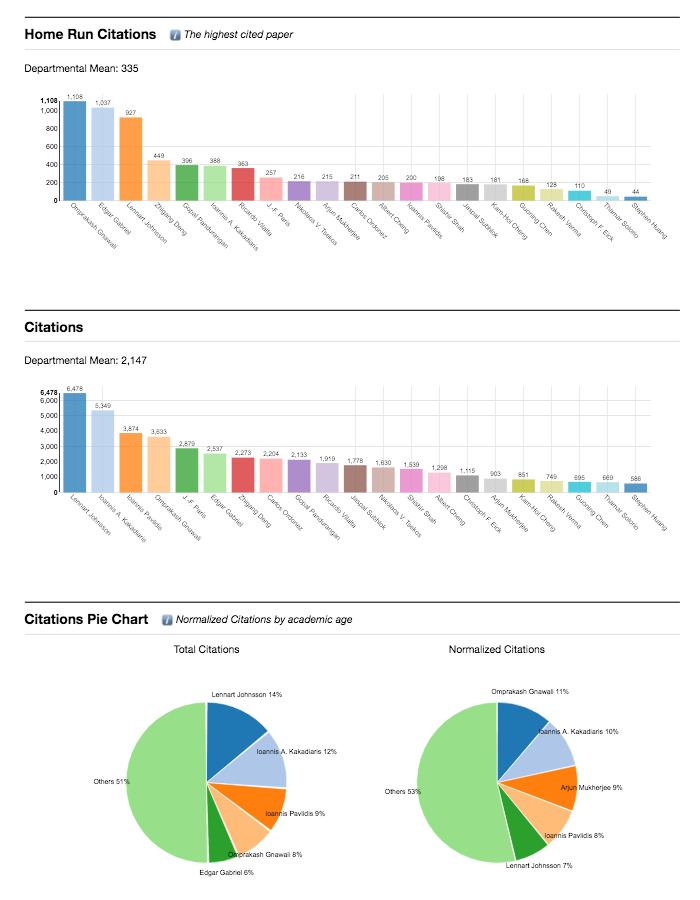
\includegraphics[width=1\textwidth]{figures/Dept-Cit}
  \caption{An example of departmnet plot - Department of Computer Science at University of Houston - Citation}~\label{fig:DP-College1}
\end{figure*}

\begin{figure*}
  \centering
  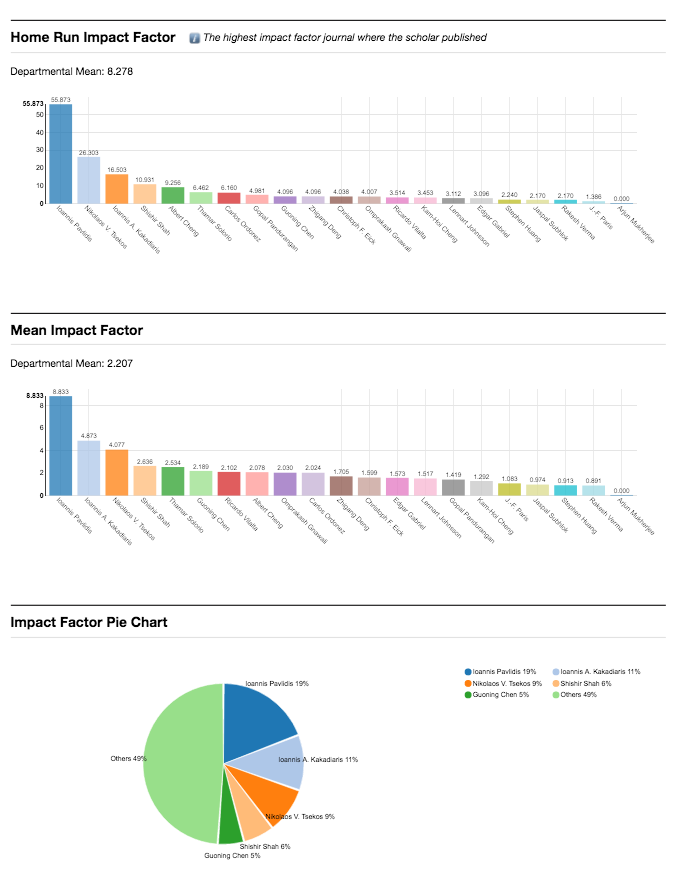
\includegraphics[width=1\textwidth]{figures/Dept-IF}
  \caption{An example of departmnet plot - Department of Computer Science at University of Houston - Impact Factor}~\label{fig:DP-College1}
\end{figure*}

\begin{figure*}
  \centering
  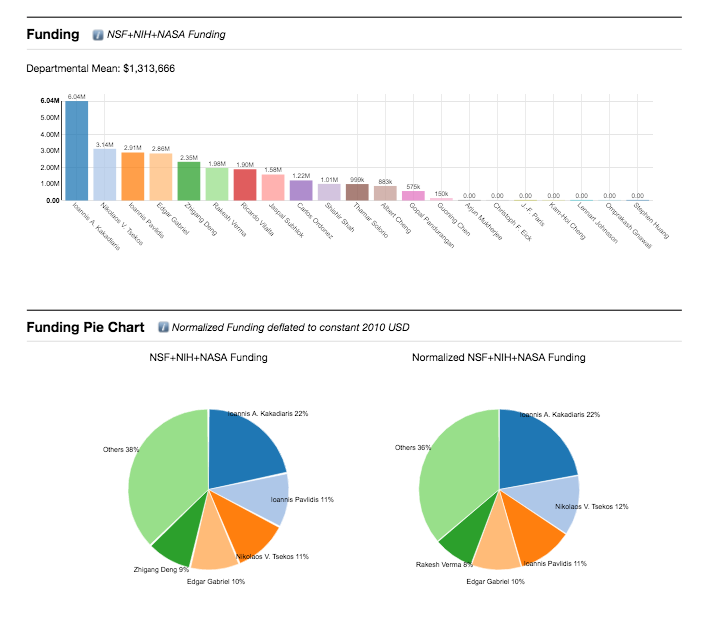
\includegraphics[width=1\textwidth]{figures/Dept-Fund}
  \caption{An example of departmnet plot - Department of Computer Science at University of Houston - Funding}~\label{fig:DP-College1}
\end{figure*}





\begin{figure*}
  \centering
  \includegraphics[width=1\textwidth]{figures/fig-Group-Citation}
  \caption{Example of Citations Pie Chart. The ones on left are at the Department Level, the ones on right are at the College Level. The charts depict total citations and normalized citations.}~\label{fig:Group-Cit}
\end{figure*}





Department Compare compares consists of comparison at the Department level. Department Compare aims to assist people to have a deeper understanding into the inner accomplishments in the departments. It complements the ranking given to the department by the US News Report. We compare the departments with the same publicly available measures. First, we compare the summary statistics like the mean values. We use boxplots to compare the distribution of values of the individual faculty in each department. We are working on extending this feature to the college level and making the user interface much more interactive.

\begin{figure*}
  \centering
  \includegraphics[width=1\textwidth]{figures/fig-GroupCompare}
  \caption{Example of Group Compare between Departments of Computer Science at University of Houston and the University of Texas - Austin.}~\label{fig:groupcompare}
\end{figure*}




%% --------------------------
\subsection{Disk Size - How to determine the size of disks}
%% --------------------------

\begin{figure}[!htb]
  \centering
  \includegraphics[width=1\textwidth]{figures/fig-Histogram-IF}
  \caption{Histogram of Impact Factor Jounal}~\label{fig:Histogram-IF}
\end{figure}

I wanted to plot to visualize more efficiently with different size of disk for Journal publications that tells the different ranking of Journal by Impact Factor Index. To do this, we analyzed the data set of JCR 2015 IF and run quartile function as a useful concept in statistics to determine the size of disks in Scholar Plot. Based on this number, the system will decide the size of plot of each journal data and plot it in real-time. The quartile values are shown in Figure \ref{fig:Histogram-IF}. The maximum number from descriptive is 153.459 through.





%Scholar Plot gives a snapshot of the individuals profile in a concise manner.
To place the plots in your personal CV or on your web page we provide a download button at the top right corner of the plot (Figure \ref{fig-scale}). This function enables the user to download plots in a zip file. It includes high resolution vector images in SVG (Scalable Vector Graphics) format of the publication and funding plots.

Scholar Plot also has a projection of the data on the y-axis depicted by small horizontal colored lines. For example, we can clearly see that journals contribute to the {\it h}-index of scholar in Figure \ref{fig:distribution} (a) and conferences / books contribute to the {\it h}-index of scholar in Figure \ref{fig:distribution} (b). We can clearly infer the scholar in Figure \ref{fig:distribution} (c)) has many patents. We can also infer the number of publications within a particular range of citations based on the density of the projected lines.

\begin{figure}[!htb]
\centering
\subfigure[]{%
\includegraphics[width=0.23\textwidth]{figures/fig_distribution_A}
}
\subfigure[]{%
\includegraphics[width=0.23\textwidth]{figures/fig_distribution_B}
}
\subfigure[]{%
\includegraphics[width=0.23\textwidth]{figures/fig_distribution_C}
}
\caption{Examples of y-axis projection for three different scholars.}~\label{fig:distribution}
  %\vspace{-1ex}
\end{figure}

%\begin{figure}[!htb]
%  \centering
%  \includegraphics[width=0.2\textwidth]{figures/fig_distribution_A}
%  \includegraphics[width=0.2\textwidth]{figures/fig_distribution_B}
%  \includegraphics[width=0.2\textwidth]{figures/fig_distribution_C}
%  \caption{Example with journals, conferences, and patents contributing to h-index}~\label{fig:distribution}
%\end{figure}

We improve user experience to enable users to quickly find and select from a pre-populated list of scholar names as they type. For each character the user enters, we display similar matching names on the dropdown list. Even entering the space (`` "), we display the 10 most recently inserted scholar's names. Scholar Plot follows the approach of responsive web design to provide optimal viewing based on the size of screen.





There are various criteria for evaluating academic performance. We focus on three main criteria. 
\begin{itemize}
\item \textbf{Impact} - it is the post-production merit. For example, the citations which a publication receives. A publication with higher number of citations has higher visibility. Therefore, we linked the impact to the vertical axis in the plot.
\item \textbf{Prestige} - this is the pre-production merit associated with the venue of publication. For example, the impact factor of a journal is the merit your publication will acquire because it has been published in that journal. Hence we associate a disk with variable sizes to the prestige of the venue. We consider it as a 'fancy factor'.
\item \textbf{Funding} - it enables the production of publications/research. Hence we place it at the bottom of the plot. This can help to correlate the production with the funding.
\end{itemize}














% ==================================================
  % \chapter{Academic Garden}\label{chap:Academic Garden}
% ==================================================
% ------------------------------------------------------------------
\section {Academic Garden - Scable Visualizatoin}
% ------------------------------------------------------------------
Academic Garden (AG) is a scalable visualization of academic merit. It applies to individual academics, departments, colleges, and any other academic group thereof, such as a research lab or a project team. Reminiscent of the legal views for physical personhood and corporate personhood, we consider that individual academics and academic groups share behavioral characteristics. Specifically, we argue that academic performance has three pillars that are scale invariant: (a) funding that enables intellectual production; (b) prestige of the venues where intellectual products appear; and, (c) impact of the intellectual products. In the case of groups, these three variables are expressed as statistics of the corresponding individual measurements.

AG uses the flower metaphor to visually articulate performance for academic entities. The width of the flower's stem is commensurate to the academic funding this entity received (`juice conduit`). The height of the flower's stem is commensurate to the impact of the entity's intellectual products (`visibility`). The diameter of the flower's disc is commensurate to the prestige of the venues where these products appeared (`fancy factor`). As secondary characteristics, the number of petal colors is commensurate to the multi-disciplinarily of the entity's intellectual production with the bud vs. bloom appearance denotes the academic entity's age.

\begin{figure*}
    \centering
    \includegraphics[width=1\textwidth]{figures/fig-Eugene-with-menu}
    \caption{Base level Scholar Plot (SP) example - a famous physicist and interdisciplinary scientist with dozen of articles in \emph{Nature}. The summary panels in the middle were added after feedback from the focus group. Notice how this scholar's publication production exploded in sync with the commencement of substantial federal funding.}~\label{fig-publication} 
\end{figure*} 

% ------------------------------------------------------------------
\subsection {Research Funding: Enabler of Production}
% ------------------------------------------------------------------
Research funding is an enabler of academic production. Very few things can be done in the absence of funding in science and engineering. Even in humanities, some funding is needed in many cases (e.g., travel support for archival research).  Research funding is dispensed through peer-reviewed proposal competitions, and for this reason it is not only an enabler but also has inherent merit. As different disciplines need different levels of funding some normalization is in order. This normalization can be any statistic. We prefer the quartile where the funding level of the academic entity's record belongs with respect to `all the records in the specific discipline. `All here is commensurate to the selected reference, whether this is a university department or a set of departments across the United States.  Needless to say that the original funding records need to be adjusted, taking into account the entity's age (if the entity is a physical person) or the number of individuals participating in the entity's personhood (if the entity is a group).

% \begin{figure*}
%     \centering
%     \includegraphics[width=1\textwidth]{figures/fig-Eugene-with-menu}
%     \caption{Base level Scholar Plot (SP) example - a famous physicist and interdisciplinary scientist with dozen of articles in \emph{Nature}. The summary panels in the middle were added after feedback from the focus group. Notice how this scholar's publication production exploded in sync with the commencement of substantial federal funding.}~\label{fig-publication} 
% \end{figure*} 

% ------------------------------------------------------------------
\subsection {Prestige of Product Venue: Pre-production Achievement}
% ------------------------------------------------------------------
Funded (and unfunded) research typically results into intellectual products. These are typically journal papers, conference proceedings papers, or books. Occasionally, intellectual products include patents or software packages, such as smartphone applications. Almost all intellectual products undergo review process, and the ones successfully passing this review process have inherent merit.  The review process criteria are not uniform. Moreover, publishing in different venues is associated with various degrees of difficulty. In journals, this difficulty is largely associated with the journal's impact factor (IF), as determined by Thomson Reuters - the higher the IF, the more difficult is to publish in a journal, and the more valuable and prestigious a potential acceptance. For refereed conferences, the prestige is loosely associated with the venue's acceptance rate - the lower the acceptance rate, the more difficult is to get into the conference proceedings, and the more prestigious the accomplishment. Unfortunately, there is no universally accepted ranking list for conferences, as is the case of the Thomson Reuters IF list for journals. Hence, it is not opportune to assign a numeric score to conference publications. The same applies for books, where evaluations are even more qualitative, and based on opinions about the perceived prestige of the publishing house. And, we are totally agnostic regarding pre-production credit, when it comes to patents and software products.

As a result, for the moment we use only IF to measure pre-production achievement. Based on histogram analysis of the frequency of publications in the IF list of journals, we use four classes to group prestige. Different grouping may be adopted, however, depending on the analytics used.

% \begin{figure*}
%     \centering
%     \includegraphics[width=1\textwidth]{figures/fig-Eugene-with-menu}
%     \caption{Base level Scholar Plot (SP) example - a famous physicist and interdisciplinary scientist with dozen of articles in \emph{Nature}. The summary panels in the middle were added after feedback from the focus group. Notice how this scholar's publication production exploded in sync with the commencement of substantial federal funding.}~\label{fig-publication} 
% \end{figure*} 

% ------------------------------------------------------------------
\subsection {Product Impact: Post-production Achievement}
% ------------------------------------------------------------------
Once a paper appears in a journal or conference proceedings, or a book appears in the market, it gets noticed and depending on how useful researchers find the concept or method contained therein, they may start using it, citing its source in their own intellectual products. This practice constitutes impact, which is a sought-after outcome of the research process as the building block of scientific advances. There are several ways of measuring impact, but the most widely accepted is the citation count.
As different disciplines have different population sizes and publication practices, which may affect citation numbers, normalization is in order. This normalization can be any statistic. We prefer the quartile where the citation count of the academic entity's record belongs with respect to `all the records in the specific discipline.  `All? here is commensurate to the selected reference, whether this is a university department or a set of departments across the United States. Needless to say that the original citation records need to be adjusted, taking into account the entity's age (if the entity is a physical person) or the number of individuals participating in the entity's personhood (if the entity is a group).


\begin{figure*}
    \centering
    \includegraphics[width=1\textwidth]{figures/fig-AG-global.png}
    \caption{Academic Garden example of Global Scale - Computer and Information Science at Northeastern University.}~\label{fig-AG-global}
\end{figure*}

\begin{figure*}
    \centering
    \includegraphics[width=1\textwidth]{figures/fig-AG-local.png}
    \caption{Academic Garden example of Local Scale - Computer and Information Science at Northeastern University}~\label{fig-AG-global}
\end{figure*}

\begin{figure}
    \centering
    \includegraphics[width=1\textwidth]{figures/fig-flower.png}
    \caption{Academic Garden Flower Diagram: A wider stem means that a flower has the necessary support to grow. The width of each stem in the plot indicates the level of funding the scholar has received. A higher quartile of funding is repesented by a wider stem and a darker green color. As a flower grows its stem heightens. The length of each stem in the plot represents a scholar's total number of citations. A flower that is flourishing produces large, colorful petals. The petals of the flowers in the plot are rendered as large brightly-colored circles. Each quartile of journal impact factor is represented by a different color, and, the higher the quartile, the larger the radius}~\label{fig-flower-diagram}
\end{figure}



% \begin{figure*}
%     \centering
%     \includegraphics[width=1\textwidth]{figures/fig-code1.png}
%     \caption{snippet}~\label{fig-publication}
% \end{figure*}


% \begin{figure*}
%     \centering
%     \includegraphics[width=1\textwidth]{figures/fig-dept-searchbox.png}
%     \caption{snippet}~\label{fig-publication}
% \end{figure*}



% \begin{figure*}
%     \centering
%     \includegraphics[width=1\textwidth]{figures/fig-AG-draft-0.png}
%     \caption{snippet}~\label{fig-publication}
% \end{figure*}

% \begin{figure*}
%     \centering
%     \includegraphics[width=1\textwidth]{figures/fig-AG-draft-1.png}
%     \caption{snippet}~\label{fig-publication}
% \end{figure*}

% \begin{figure*}
%     \centering
%     \includegraphics[width=1\textwidth]{figures/fig-AG-draft-2.png}
%     \caption{snippet}~\label{fig-publication}
% \end{figure*}

% \begin{figure*}
%     \centering
%     \includegraphics[width=1\textwidth]{figures/fig-AG-draft-3.png}
%     \caption{snippet}~\label{fig-publication}
% \end{figure*}















% ==================================================
\chapter{Software Engineering}\label{chap:Software Engineering}
% ==================================================

% --------------------------
\section{Data Sources}
% --------------------------
There were several options to get bibliographic data for powering the publication plot of Scholar Plot (SP). These included \href{http://www.scopus.com/}{Scopus}, \href{http://www.isiknowledge.com/}{ISI Web of Knowledge}, and \href{http://scholar.google.com}{Google Scholar}. We chose Google Scholar for two reasons: a) it is all inclusive, covering all types of publications, that is, journals, conferences, books, and patents; and, b) it is freely available. Scopus is subscription based and not as inclusive as Google Scholar. ORCID has publications and funding data but requires extensive set-up.

Our choice carries a few challenges, too. Google Scholar does not provide an application programming interface. Hence, we had to develop elaborate software to scrape information off publicly available Google Scholar pages. Also, not every academic has a Google Scholar page. This has been changing fast, however, as one college after the other in the United States mandating their faculty to maintain a Google Scholar page.

We use the Journal IF List issued every year by Thompson Reuters to assign disk sizes to journal publications.

For funding records, we use the publicly available grant records from the National Science Foundation (NSF) \cite{nsf}, the National Institutes of Health (NIH) \cite{nih}, and the National Aeronautics and Space Administration (NASA) \cite{nasa}. These are the only funding agencies with publicly available datasets at this point.

11,867 records in our database.

\begin{table}[h!]
\centering
\begin{tabular}{||c c c c||}
 \hline
 Agencies & Fiscal Year & Rows & Per Year \\ [1ex]
 \hline\hline
 NSF & FY 1985 - FY 2013 & 312,311 rows & 10,769/year \\
 NIH & FY 2000 - FY 2013 & 777,657 rows & 55,456/year \\
 NASA & FY 2007 - FY 2015 & 16,670 rows & 1,852/year \\ [1ex]
 \hline
\end{tabular}
\caption{Funding datasets in Scholar Plot system.}
\label{table:1}
\end{table}









% --------------------------
\section{System Architecture}
% --------------------------


Scholar Plot is the web-based data visualization mothod that uses HTML5, CSS3 and SVG to render a scholar's accomplishment at a glance. We created a MySQL database to store the mapping between the scholar names and their Google Scholar IDs. We also designed and created database tables for NSF/NIH/NASA funding data. The user can search the name of the scholar in a text field. When the user starts to enter the name of the scholar, the names in our database which are similar to the entered name will be listed as a drop down list. We use jQuery and Ajax (asynchronous JavaScript and XML) method to have this feature, which connects to the database to get the list of names. If there are no matching/similar names, the user can also insert her/his Google Scholar ID to the database by one click event.

\begin{figure}[H]
\centering
  \includegraphics[width=1\textwidth]{figures/fig_system_architecture.pdf}
  \caption{System Architecture of Scholar Plot.}~\label{fig-arch}
%\vspace{-1ex}
\end{figure}

Once the scholar's name selected, the user can run the application to see the visual results of the selected scholar's publications and fundings. Scholar Plot connects to the Web server to retrieve the necessary information.
The server-side application is implemented in PHP scripting language and MySQL. The HTTP protocol is used for communicating between client-side and server-side to get the basic information via JSON format (JavaScript Object Notation) and JSONP function (Figure \ref{fig-arch}). Scholar Plot also uses htmlSQL library to parse Google Scholar's page to extract user basic information \cite{htmlSQL}.

%, collecting for the publication title, the journal name, the co-authors' name, the year, and the citations. It also collects the {\it h-}index and the number of total citations from the top of the scholar's page up to 300 publications.

Scholar Plot obtains the Impact Factor ($IF$) for a particular journal from our database. The data of Impact Factor is acquired from The Thomson Reuters Impact Factor - Web of Science. Based on all this information it constructs the plots as per the design outlined in the Visualization and User Interface section, using nvd3 library \cite{nvd3org}.

The NSF/NIH/NASA funding datasets are available at the respective US government websites in various file formats such as XML, CSV and so on \cite{nsf, nih, nasa}. We implemented a script to parse this massive XML dataset into our data structure that consists of AwardID, AwardAmount, First name, Last name, Investigator by RoleCode (Principal Investigator, Co-Principal Investigator and Former Principal Investigator), using XMLStarlet \cite{XMLStarlet}. We imported this data to our database using Toad DBMS tool. Currently, we have only these three funding data sources. So this is a limitation of the current system. It is biased to the scholar's country of residence. We are working on adding more of them to our database. %We designed our relational database schema in MySQL.




% ==================================================
% \chapter{Algorithms}\label{chap:Algorithms}
% ==================================================
% --------------------------
\section{Name Disambiguation}
% --------------------------


With the amount of data and data sources rapidly growing and expanding, it is essential for the large amounts of available data to be organized for analysis. Through the process known as Data Wrangling, unorganized and scattered data can be prepared for easy access and analysis. The datasets of google and goverment funding have to be cleaned because it contains many non-english characters and its messy datasets \ref{kang2008interactive}. We use regular expression to remove the invalid special characters and translate phonetic characters to english alphabets. We designed and implemented Algorithms \ref{algorithm} to match the author names in Google Scholar with those in NSF/NIH/NASA data. This process helps to improve the quality of results.


\subsection{Within the Google Scholar profile}

A single Google Scholar profile might contain multiple variations of the authors name based on the middle name and initials. For example, consider the example Google Scholar profile of Ioannis Pavlidis. It contains four variations of his name in different publications.

\begin{itemize}
\item Ioannis T Pavlids
\item IT Pavlids
\item I Pavlids
\item Ioannis Pavlids
\end{itemize}

We use the first initial and last name of an author to obtain the count of the number of publications in the panel.

\begin{figure}[H]
\begin{center}
  \includegraphics[width=.9\textwidth]{figures/fig-name-dis-example1}
\caption{Example of how the name disambiguation algorithm works.}
\label{default}
\end{center}
\end{figure}




% --------------------------
\subsection{Between Google Scholar and Funding datasets}
% --------------------------

The funding datasets released from governments need to be cleaned because their different data formats and structure. We cleaned the names by removing Jr., III, PhD, Dr., and so on. Then we need to match the names in the Google Scholar profile with those in the funding datasets. The algorithm is given in Algorithm \ref{algorithm}. An example is visually depicted in Figure \ref{alg-example}.

\begin{figure}
\begin{algorithm}[H]
\caption{Matching the name between Google Scholar and funding datasets}
\begin{algorithmic}[1]
\Procedure{Searching for Author Name}{}
\State $\textit{googleFirstName} \gets \text{first name in Google Scholar }$
\State $\textit{googleLastName} \gets \text{last name in Google Scholar }$
\State $\textit{googleMiddleInitial} \gets \text{middle initial in Google Scholar }$
\If {$lastNameInFundingData = googleLastName$}
\If {$firstNameInFundingData = googleFirstName$} 
\If {$googleMiddleInitial$ is null } 
{\Return true}
\Else{
\text{Search for} ($middleInitial, googleFirstName$) and ($googleFirstName, middleInitial$) 
\If { $found$} \Return true
\Else{ \Return false}
\EndIf
}
\EndIf
\EndIf
\EndIf
\Return false
\EndProcedure
\label{algorithm}
\end{algorithmic}
\end{algorithm}
\end{figure}



\begin{figure}[H]
\begin{center}
  \includegraphics[width=.9\textwidth]{figures/fig-name-dis-example2}
\caption{Example of matching the name in Google Profile with the name in funding data. Daniel M. Smith is considered as Daniel Michael Smith and Daniel Smith.}
\label{alg-example}
\end{center}
\end{figure}




% --------------------------
\subsection{Within and across profile author name disambiguation}
% --------------------------

Let $i$ be an index for the Google scholar profile researchers. Within each collaboration profile of $i$,  there are a set of $K_{0}$ raw name strings that you have extracted,  $Names_{k}$ indexed by $k_{i}$. We will use the fact that these strings are associated with profile $i$ in the process of name disambiguation across Google Scholar profiles. The following provides an outline of this procedure: \\


A) {\bf Clean last names:}
Remove strings at end of all $Names_{k}$ that are not last names, and which may not consistently be listed for $k$, e.g. ``Jr.'', ``III'' etc. Hence, each name string  $Name_{k}$ consists ideally of a First name string $FN_{k}$, a Last name string $LN_{k}$, and possibly a Middle name string $MN_{k}$. \\

B)  {\bf Clean middle initial strings within each profile $i$:}  Within each $i$, search for inconsistencies in the use of $MN_{k}$. That is, possibly sometimes the author $k$ is listed as {\it Alexander M Petersen}, sometimes {\it Alexander Petersen}, and sometimes {\it Alexander Michael Petersen}. In this example the Last name string $LN_{k} = Petersen$ and the First name string $FN_{k} = Alexander$ are clearly consistent. But the Middle name string \{$\_$ , M, Michael\} causes some ambiguity if simple string comparison is used,  where $\_$ is a whitespace.

%Hence, for each distinct  surname $FN_{k}$ and last name $LN_{k}$, map all $MN_{k}$ strings to the simplest representation $\hat X$ of just the middle name initials.\\

Then check to see how many different types of {\it Alexander} $\hat X$ {\it Petersen} occur within each $k$, where $\hat X$ is refers to the middle name. Use the following rules for when there are 2 or more types of $\hat W \hat X Petersen$.

 \begin{itemize}
 \item If there are only two  types of $Alexander \hat X Petersen$, with $\hat X=$ $\_$ or $M$, then map all of the $Alexander \hat X Petersen$ to $Alexander M Petersen$ for this $i$
 \item If there are only three types of $Alexander \hat X Petersen$, with $\hat X=$ starting with the same initial, $M\_$ or $M$, then map all of the $A\hat X Petersen$ to $Alexander Michael Petersen$ for this $i$
 \item If there are two or more types of $Alexander \hat X Petersen$, say $\hat X=O$ and $\hat X=P$, then keep these $X$ as they are.

%  \item However, if one of those types are a whitespace,  say $\hat X=O$ and $\hat X=P$  and $X= \_$, then we cannot know if the latter possibly corresponds to $O$ or $P$. This case shouldn't occur often. So we can use the simple heuristic that if there is any paper with $AO$ and $A$, then in this case the latter is actually $AP$, and so all $A\_$ are mapped to $AP$. If there are no papers that make obvious this distinction,  then compare the coauthors of $AO$ and $AP$  and $A \_$ within the profile of $i$. Map $A \_$ to $AP$ if they share more coauthors or map $A \_$ to $AP$ if they share more coauthors using the Jaccard Similarity measure to compare.
\end{itemize}

C)  {\bf Disambiguate coauthors $k$ across the Google Scholar profiles (connecting $i$):} Let  $k$ and $k'$ be coauthors in profiles $i$ and $i'$, respectively.   In this step we would like to identify $k$ and $k'$ that are likely the same person, $k=k'$, allowing us to connect the two profiles $i$ and $i'$ within the coauthor network.\\

 If $k$ and $k'$ have the same initials and same surname, then there is a possibility that they are the same individual. Also, if their full first name strings match, this is clearly very positive evidence of this. Let $A_{k,j}$ be the entire combination of First Name and Middle initial $FM_{k,j}$ with the surname $L_{k,j}$ (e.g. {\it Adam B Smith}, or {\it Adam \_ Johnson}) of the coauthor $j$ of the coauthor $k$.

 \begin{itemize}
 \item If the full first name strings and the full last name strings are the same, $FN_{k,j}$=$FN_{k',j}$ and $LN_{k,j} = LN_{k',j}$ (e.g. Adam J. Johnson and Adam Johnson), and they both have at least one coauthors in common,  then they are considered the same coauthor.
 \item If we don't have the added information of their full first names then we must rely more heavily on the information from their coauthors. If the first and last names are the same, $FM_{k,j}=FM_{k',j}$ and $LM_{k,j}=LM_{k',j}$, and there are more than 2 middle names with one of the middle name being empty, we do the following -

 We compute the number of coauthors in common of the empty middle name author with non-empty middle name authors by comparing the sets of coauthors, $\{j\}$.% and $\{j'\}$.

 We assign the empty middle name to that middle name for which there are more number of co-authors in common.

 \item If the first name of the author has a hyphen, we check for any other author having the same last name and the first name as the first word of the hyphenated word and middle name starting with the first letter of the second part of the hyphenated word. If any such pair of authors have at least one author in common, we update the first and middle name of the author with the hyphenated middle name to first name and middle name of the matched author.


\item If the first name of the author has only two letters, we check for any other author having the same last name and the first name starting with the first letter of the first name and middle name starting with the second letter of the first name. If any such pair of authors have at least one author in common, we update the first and middle names of the author with two letters to first and middle names of the matched author.

\end{itemize}
Google Scholar data has to be cleaned because it contains many non-english characters. We use regular expression to remove the invalid special characters and translate phonetic characters to english alphabets. We designed and implemented Algorithm \ref{alg:name} to match the author names in Google Scholar with those in NSF/NIH/NASA data. This process helps to improve the quality of results.







% ==================================================
\chapter{Results}\label{chap:Results}
% ==================================================

% --------------------------
\section{User Feedback - Usability Study}
% --------------------------



A total of 15 participants from various disciplines including Natural Sciences, Social Sciences, Life Sciences and Computer Science evaluated Scholar Plot. We asked each participant to review the interface and then complete an online survey. Special care was taken to ensure that the participants had correct understanding about the visualization component before they began rating. The participants answered the questions on a Likert scale from 1 to 5 with 1 being strongly disagree and 5 being strongly agree.

Figure \ref{fig:UserStudy} illustrates the mean evaluation for each visualization component. Accuracy, Usability and understandability of Scholar Plot scored the highest $(\mu = 4.2)$ as it is very intuitive and can be used with minimal assistance. Many participants gave us feedback that they mostly liked the visual scheme of Scholar Plot. Another observation is that the participants agree to use Scholar Plot to evaluate themselves $(\mu = 4.1)$. They suggested that Scholar Plot can be improved by adding more funding agencies. Overall, this evaluation indicated that Scholar Plot is a user-friendly tool that complements the CV which can be used to review a scholar's accomplishments. The survey has been approved by the University of Houston Institutional Review Board (IRB).

 \begin{figure}[!htb]
  \centering
  \includegraphics[width=\textwidth]{figures/fig_survey_chart}
%  \vspace{-3ex}
  \caption{Mean evaluation of Scholar Plot. A total of $n=15$ participants evaluated the survey.}
  \label{fig:UserStudy}
\end{figure}



% --------------------------
\section{User Feedback - Focus Group}
% --------------------------

We ran a focus group with 10  Principal Investigators and their post docs at Northwestern University. The participant set included biologists, physicists, computer scientists, and social scientists.  The focus group's suggestions are synopsized as follows:
\begin{description}
\item [Interface team science information.] Participants wanted to see the number and intensity of collaborations for the depicted scholar.
\item [Summarize highly cited papers.] Participants wanted to see explicitly in a side panel the scholar's most popular papers.
\item [Interface journal profile.] Participants wanted to see the specific journals where the scholar publishes most often and their impact factors.
\end{description}

The participants believed that accessorizing the central publication graph with this additional information would support deeper instant comprehension without compromising the elegance of SP's compact visual representation. Specifically, this additional interface would reveal the collaborative nature of the scholar's work, give hints if s/he is regular in specific disciplinary journals or if s/he publishes in a variety of journals (interdisciplinarity), and give the rank of these journals. All this information can also be gleaned by rolling the mouse over the publication graph, reading the tooltips; summarizing it in panels under the graph, however, renders such manual investigation unnecessary.

\begin{figure}[H]
    \centering
    \includegraphics[width=\textwidth]{figures/fig_panel1-N}
    \caption{Panel listing the top collaborators with the selected scholar ranked by the count of the number of publications collaborated.}
    \label{fig:panel1}
\end{figure}

\begin{figure}[H]
    \centering
    \includegraphics[width=\textwidth]{figures/fig_panel3-N}
    \caption{Panel highlighting the top 5 cited papers of the selected scholar.}
    \label{fig:panel3}
\end{figure}

\begin{figure}[H]
    \centering
    \includegraphics[width=\textwidth]{figures/fig_panel2-N}
    \caption{Panel displaying the top journals ranked by the frequency of publication.}
    \label{fig:panel2}
\end{figure}

\begin{figure}[H]
    \centering
    \includegraphics[width=\textwidth]{figures/fig_panel4-N}
    \caption{Panel showing the top 5 journals where the selected scholar published ranked by the impact factor.}
    \label{fig:panel4}
\end{figure}






% --------------------------
\section{Academic Garden Validation - Chaired Faculty }
% --------------------------

In progress....






% ==================================================
\chapter{Conclusion}\label{chap:Conclusion}
% ==================================================
We have described a visualization method that complements the information contained in a researcher's Google Scholar page and summarized by her/his {\it h}-index. One can draw insightful conclusions about the individual's scholastic accomplishments. These conclusions are not supported by the {\it h}-index alone and cannot be derived by the CV or the Google Scholar page, unless a significant investigative effort is undertaken. Our user study also supports this.

This approach not only focusses on journal publications, conferences / books and patents but also NSF/NIH/NASA funding data. Scholar Plot is a simple, yet valuable visualization scheme. It is likely to have broad appeal not only because it would be useful to evaluation committees, but also because it is available online for free at \url{http://www.scholarplot.com}.


I presented Scholar Plot (SP), a scalable (individual-department-college) visualization interface for academic merit. I have released Scholar Plot at \href{http://scholarplot.com}{http://scholarplot.com}.

Scholar Plot works at three levels - the individual, the department, and the college. The individual (base) level captures in a figure three key indicators of academic prowess: citation impact, prestige of publication venues, and research funding. These indicators scale up in the department \& college (aggregate) levels of Scholar Plot as pie charts, revealing at a glance the relative contributions of entities from the lower echelon.

The basic idea behind Scholar Plot is to facilitate instant deeper comprehension regarding different strengths of academic records, supporting the work of evaluation committees and the curious academic in search of an advisor or department. One of SP's strengths is that it draws data from open sources that are inclusive. This creates, however, a technical problem because Google Scholar - a key open source used by SP - does not offer an application programming interface. For the base level of SP we solved this problem with sophisticated data scraping assisted by a simple one-time wiki function: if the individual sought by the user is not recognized by SP, then SP asks the user to copy and paste the targeted individual's Google Scholar URL; SP remembers it thereafter, automatically scraping the scholar's data every time a user requests it by name. For the department and college levels, a wiki function is in the works.

A focus group and a survey study indicated that the base level of SP is well received by academics. We plan to conduct a longitudinal study of SP users, to further inform the design cycle.

% Academic Garden is available on the top of department plot and it illustrats 



% --------------------------
\chapter{Appendix}
% --------------------------


% --------------------------
\section{Usage of Scholar Plot}
% --------------------------
In this section, I will explain how to access and use Scholar Plot. This includes searching for a scholar from Google, inserting a scholar, obtaining results, and the scholar's profile URL.

% --------------------------
\subsection{Searching for a scholar}
% --------------------------
To visualize the accomplisments of a scholar, type the name of a scholar in the search box. As you type, Scholar Plot will attempt to match your query to the names of scholars in our system.

\begin{figure*}[hb]
  \centering
  \includegraphics[width=1\textwidth]{figures/Support-3}
  \caption{An example of Scholar Plot - Type the name of a scholar in the search box}~\label{fig:Support-3}
  % \vspace{-2ex}
\end{figure*}

If the result of a search produces no results, Scholar Plot will prompt you to enter the URL of the person's Google Scholar Citations Profile. Instructions for finding a Google Scholar URL can be found.


\begin{figure*}
  \centering
  \includegraphics[width=1\textwidth]{figures/Support-4}
  \caption{An example of Scholar Plot - No Results in Scholar Plot Search}~\label{fig:Support-4}
  % \vspace{-2ex}
\end{figure*}




% --------------------------
\subsection{If a name cannot be found}
% --------------------------
When a name cannot be found in our system, Scholar Plot will prompt the user to enter the URL of the person's Google Scholar Citations Profile. This URL can be found using the search bar on the Google Scholar website (here\href{https://scholar.google.com/citations?mauthors=&hl=en&view_op=search_authors}).

If the names of more than one scholar match the query, you will need to locate the correct scholar in the search results.



% --------------------------
\subsection{Google Scholar Author Search Results}
% --------------------------
From the person's Google Scholar Citations Profile page, copy the URL from your web browser's address bar.

\begin{figure*}
  \centering
  \includegraphics[width=1\textwidth]{figures/Support-1}
  \caption{An example of Scholar Plot - Visualizing Funding Data}~\label{fig:Support-1}
  % \vspace{-2ex}
\end{figure*}




% --------------------------
\subsection{Obtaining the Google Scholar Profile URL}
% --------------------------
Return to Scholar Plot and click the `Submit` button. The scholar's information will then appear and their name can be used in future searches on Scholar Plot and Scholar Compare.

\begin{figure*}
  \centering
  \includegraphics[width=1\textwidth]{figures/Support-2}
  \caption{An example of Scholar Plot - Copying the Google Scholar Citations Profile URL}~\label{fig:Support-2}
  % \vspace{-2ex}
\end{figure*}

\begin{figure*}
  \centering
  \includegraphics[width=1\textwidth]{figures/Support-5}
  \caption{An example of Scholar Plot - Pasting the Google Scholar Citations Profile URL}~\label{fig:Support-5}
  % \vspace{-2ex}
\end{figure*}





% \lstinputlisting[language=SQL, caption=Cption]{./codes/Disambiguation-step1.sql}
% \lstinputlisting[language=SQL]{./codes/Disambiguation-step2.sql}
% \lstinputlisting[language=SQL]{./codes/Disambiguation-step3.sql}
% \lstinputlisting[language=SQL]{./codes/Disambiguation-step4.sql}
% \lstinputlisting[language=SQL]{./codes/Disambiguation-step5.sql}



%\section{Summary of Contributions}
%
%\subsection{Image Segmentation}
%
%\subsection{Cardiac Morphology and Function}
%
%\subsection{Coronary Artery Shape-Motion Analysis}
%
%%%%%%%%%%%%%%%%%%%%%%%%%%%%%%%%%%%%%%%%%%%%%%%%%%%%%%%%%%%%%%%%
%\section{Progression and Scope for Future Work}
%
%
%\subsection{Algorithm for the Automatic LV Blood Pool Segmentation
%from Short-Axis Dual-Contrast MR Data}
%
%%%%%%%%%%%%%%%%%%%%%%%%%%%%%%%%%%%%%%%%%%%%%%%%%%%%%%%%%%%%%%%%
%\subsection{Algorithm for the Automatic Delineation of Myocardial
%Contours in Short-Axis Cardiac Cine-bFFE MR Sequences}
%
%
%%%%%%%%%%%%%%%%%%%%%%%%%%%%%%%%%%%%%%%%%%%%%%%%%%%%%%%%%%%%%%%%
%\subsection{Algorithm for the Automatic Computation of EF from the Short-Axis Cardiac Cine-bFFE MR Sequences}
%
%
%%%%%%%%%%%%%%%%%%%%%%%%%%%%%%%%%%%%%%%%%%%%%%%%%%%%%%%%%%%%%%%%
%\subsection{Computational Framework for the 4D
%Shape-Motion Analysis of the LAD}
%
%
%%%%%%%%%%%%%%%%%%%%%%%%%%%%%%%%%%%%%%%%%%%%%%%%%%%%%%%%%%%%%%%%
%\subsection{Future Work}
%
%%%%%%%%%%%%%%%%%%%%%%%%%%%%%%%%%%%%%%%%%%%%%%%%%%%%%%%%%%%%%%%%


% --------------------------
\chapter{Appendix}
% --------------------------


% --------------------------
\section{Usage of Scholar Plot}
% --------------------------
In this section, I will explain how to access and use Scholar Plot. This includes searching for a scholar from Google Scholar, inserting a scholar into our system, obtaining results, and the scholar's profile URL.

% --------------------------
\subsection{Searching for a scholar}
% --------------------------
To visualize the accomplishments of a scholar, type the name of a scholar in the search box. As you type, Scholar Plot will attempt to match your query to the names of scholars in our system.

\begin{figure*}[hb]
  \centering
  \includegraphics[width=1\textwidth]{figures/Support-3}
  \caption{Usage of Scholar Plot - Type the name of a scholar in the search box.}~\label{fig:Support-3}
  % \vspace{-2ex}
\end{figure*}

If the result of a search produces no results, Scholar Plot will prompt you to enter the URL of the person's Google Scholar Citations Profile. Instructions for finding a Google Scholar URL can be found.


\begin{figure*}
  \centering
  \includegraphics[width=1\textwidth]{figures/Support-4}
  \caption{Usage of Scholar Plot - No Results in Scholar Plot Search in Scholar Plot System.}~\label{fig:Support-4}
  % \vspace{-2ex}
\end{figure*}




% --------------------------
\subsection{If a name cannot be found}
% --------------------------
When a name cannot be found in our system, Scholar Plot will prompt the user to enter the URL of the person's Google Scholar Citations Profile. This URL can be found using the search bar on the Google Scholar website (\href{https://scholar.google.com/citations?mauthors=&hl=en&view_op=search_authors}here).

If the names of more than one scholar match the query, you will need to locate the correct scholar in the search results.



% --------------------------
\subsection{Google Scholar Author Search Results}
% --------------------------
From the person's Google Scholar Citations Profile page, copy the URL from your web browser's address bar.

\begin{figure*}
  \centering
  \includegraphics[width=1\textwidth]{figures/Support-1}
  \caption{Usage of Scholar Plot - Searching a scholar profile in Google Scholar.}~\label{fig:Support-1}
  % \vspace{-2ex}
\end{figure*}




% --------------------------
\subsection{Obtaining the Google Scholar Profile URL}
% --------------------------
Return to Scholar Plot and click the `Submit' button. The scholar's information will then appear and their name can be used in future searches on Scholar Plot and Scholar Compare.

\begin{figure*}
  \centering
  \includegraphics[width=1\textwidth]{figures/Support-2}
  \caption{Usage of Scholar Plot - Copying the Google Scholar Citations Profile URL.}~\label{fig:Support-2}
  % \vspace{-2ex}
\end{figure*}

\begin{figure*}
  \centering
  \includegraphics[width=1\textwidth]{figures/fig-paste}
  \caption{Usage of Scholar Plot - Pasting the Google Scholar Citations Profile URL.}~\label{fig:Support-5}
  % \vspace{-2ex}
\end{figure*}

\bibliographystyle{abbrv}
\bibliography{kkwon2}
\end{document}
